\documentclass{report}

\usepackage[T1]{fontenc}
\usepackage[utf8]{inputenc}
\usepackage{times}

\usepackage[font=small,labelfont=bf,tableposition=top]{caption}
\usepackage{graphicx}
\usepackage{natbib} 

\usepackage{amsmath}
\usepackage{amsfonts}
\usepackage{amssymb}
\usepackage{color, soul}
\usepackage{hyperref}
\usepackage{algorithmicx}
\usepackage{algpseudocode}
\usepackage{subfigure}
\usepackage{stmaryrd}

\renewcommand{\vec}[1]{\boldsymbol{{#1}}} 
\newcommand{\duesoon}[1]{{\sethlcolor{green}\hl{#1}}}
\usepackage{mathrsfs}


\newtheorem{theorem}{Theorem}
\newtheorem{acknowledgement}[theorem]{Acknowledgement}
\newtheorem{algorithm}[theorem]{Algorithm}
\newtheorem{axiom}[theorem]{Axiom}
\newtheorem{case}[theorem]{Case}
\newtheorem{claim}[theorem]{Claim}
\newtheorem{conclusion}[theorem]{Conclusion}
\newtheorem{condition}[theorem]{Condition}
\newtheorem{conjecture}[theorem]{Conjecture}
\newtheorem{corollary}[theorem]{Corollary}
\newtheorem{criterion}[theorem]{Criterion}
\newtheorem{definition}[theorem]{Definition}
\newtheorem{example}[theorem]{Example}
\newtheorem{exercise}[theorem]{Exercise}
\newtheorem{lemma}[theorem]{Lemma}
\newtheorem{notation}[theorem]{Notation}
\newtheorem{problem}[theorem]{Problem}
\newtheorem{proposition}[theorem]{Proposition}
\newtheorem{remark}[theorem]{Remark}
\newtheorem{solution}[theorem]{Solution}
\newtheorem{summary}[theorem]{Summary}
\newenvironment{proof}[1][Proof]{\textbf{#1.} }{\ \rule{0.5em}{0.5em}}

\newtheorem{guess}{Definition}
\newcommand{\comment}[1] {}
\newcommand{\Norder} {N}
\newcommand{\order}{\mathcal{O}}
\newcommand{\Npoints} {N_p}
\newcommand{\Nfaces} {N_{f}}
\newcommand{\Nelements} {N_e}

\newcommand{\eps}{\varepsilon}
\newcommand{\Dweak}{\wt{D}}
\newcommand{\diff}[2] {\frac{\partial #1}{\partial #2}}
\newcommand{\dxx}[2] {\frac{\partial^2 #1}{\partial {#2}^2}}
\newcommand{\difft}[2] {\frac{d #1}{d #2}}
\newcommand{\dxxt}[2] {\frac{d^2 #1}{d {#2}^2}}
\newcommand{\lagrange}[1] {\frac{d #1}{dt}}
\newcommand{\lebesgue}{\parallel I \parallel}
\newcommand{\polysp}{\mathcal{P}_N}
\newcommand{\laplacian}{\nabla^2}
\newcommand{\divergence}{\nabla \cdot}
\newcommand{\inte}{\int_{\mbox{\footnotesize ${\Omega_e}$}}}
\newcommand{\intb}{\int_{\mbox{\footnotesize ${\Gamma_e}$}}}
\newcommand{\intce}{\int_{\mbox{\footnotesize ${\widehat{\Omega}_e}$}}}
\newcommand{\intcb}{\int_{\mbox{\footnotesize ${\widehat{\Gamma}_e}$}}}
\newcommand{\intg}{\int_{\mbox{\footnotesize ${\Omega}$}}}
\newcommand{\intgb}{\int_{\mbox{\footnotesize ${\Gamma}$}}}
\newcommand{\intv}{\int_{\mbox{\footnotesize ${\sigma}$}}}
\newcommand{\sumv}{\sum_{K=1}^{N_{\mathrm{lev}}}}
\newcommand{\sumk}{\sum_{L=1}^{K}}
\newcommand{\sumN}{\sum_{i=1}^{N+1}}
\newcommand{\half}{\frac{1}{2}}
\newcommand{\inti}{\int_{\mbox{\footnotesize\sf I}}}
\newcommand{\intbd}{\oint_{\mbox{\footnotesize ${\delta}$\sf D}}}
\newcommand{\intbi}{\oint_{\mbox{\footnotesize ${\delta}$\sf I}}}
\newcommand{\ldnorm}[1]{\left\| #1 \right\|_{\mbox{\footnotesize \sf D}} }
\newcommand{\lonorm}[1]{\left\| #1 \right\|_{\Omega}}
\newcommand{\spc}[1]{\mbox{\sf #1}}
\newcommand{\ope}[1]{{\cal #1}}
\newcommand{\mt}[1]{{\rm #1}}
\newcommand{\dis}{\displaystyle}
\newcommand{\ve}{\varepsilon}
\newcommand{\ov}{\overline}
\newcommand{\wt}{\widetilde}
\newcommand{\wh}{\widehat}
\newcommand{\Dhat}{\widehat{D}}
\newcommand{\be}{\begin{equation}}
\newcommand{\ee}{\end{equation}}
\newcommand{\bea}{\begin{eqnarray*}}
\newcommand{\eea}{\end{eqnarray*}}
\newcommand{\Jace}{J^{(e)}}
\newcommand{\Jacl}{J^{(l)}}
\def\bepsilon{\mbox{\boldmath $\epsilon $}}
\def\bpsi{\mbox{\boldmath $\psi $}}
\def\bphi{\mbox{\boldmath $\phi $}}
\def\bmu{\mbox{\boldmath $\mu $}}
\def\Et{ \tilde{E} }
\def\Ht{ \tilde{H} }
\def\sdot{ \dot{\sigma} }

\newcommand{\fstar}{f^{(*)}}

\DeclareMathOperator{\Span}{span}
\DeclareMathOperator{\Dim}{dim}

\newcommand{\polyquad}{\mathcal{Q}_{N}}
\newcommand{\polyP}{\mathcal{P}_{N}}
\newcommand{\polyPnpm}{\mathcal{P}_{(N+M)}}
\newcommand{\polyPd}{\mathcal{P}_{d}}
\newcommand{\polyPnm}{\mathcal{P}_{N,M}}
\newcommand{\polyPn}{\mathcal{P}_{N,0}}
\newcommand{\transpose}{^{\mathcal{T}}}

\newcommand{\vecQ}{\vec{Q}}
\newcommand{\vecQe}{\vec{Q}^{(e)}}
\newcommand{\vecFe}{\vec{\mathcal{F}}^{(e)}}
\newcommand{\statevec}{\vec{Y}}
\newcommand{\statevecN}{\vec{Y}_N^{(e)}}
\newcommand{\statestage}{\vec{\mathcal{Y}}}
\newcommand{\Ftensor}{\vec{F}(\qvector)}
\newcommand{\FtensorN}{\vec{F}\left( \qvectorN \right)}
\newcommand{\FtensorStar}{\vec{F}\left( \qvector_N^{(e,k)} \right)}
\newcommand{\Svector}{S(\qvector)}
\newcommand{\SvectorN}{S \left( \qvectorN \right)}
\newcommand{\qref}{\vec{q}_0}
\newcommand{\qvectorb}{\vec{q}_b}
\newcommand{\qtt}{\vec{q}_{tt}}
\newcommand{\qhat}{\widehat{\vec{q}}}
\newcommand{\qhatb}{\widehat{\vec{q}}_b}
\newcommand{\qelem}{q^{(e)}}
\newcommand{\rhoref}{\rho_0}
\newcommand{\piref}{\pi_0}
\newcommand{\Thetaref}{\Theta_0}
\newcommand{\Gref}{G_0}
\newcommand{\Tref}{T_0}
\newcommand{\thetaref}{\theta_0}
\newcommand{\Pref}{{P}_0}
\newcommand{\Eref}{{E}_0}
\newcommand{\Href}{{h}_0}
\newcommand{\rhohat}{\widehat{\rho}}
\newcommand{\pihat}{\widehat{\pi}}
\newcommand{\Phat}{\widehat{P}}
\newcommand{\uvechat}{\widehat{{\mbox{\boldmath$u$\unboldmath}}}}
\newcommand{\uhathat}{\widehat{\widehat{{\mbox{\boldmath$u$\unboldmath}}}}}
\newcommand{\Uhat}{\widehat{{\mbox{\boldmath$U$\unboldmath}}}}
\newcommand{\Uhathat}{\widehat{\widehat{{\mbox{\boldmath$U$\unboldmath}}}}}
\newcommand{\thetahat}{\widehat{\theta}}
\newcommand{\Thetahat}{\widehat{\Theta}}
\newcommand{\Ehat}{\widehat{E}}
\newcommand{\uhat}{\widehat{u}}
\newcommand{\vhat}{\widehat{v}}
\newcommand{\what}{\widehat{w}}
\newcommand{\pitt}{\pi_{tt}}
\newcommand{\rhott}{\rho_{tt}}
\newcommand{\Ett}{E_{tt}}
\newcommand{\Utt}{\vec{U}_{tt}}
\newcommand{\uvectt}{\vec{u}_{tt}}
\newcommand{\utt}{u_{tt}}
\newcommand{\vtt}{v_{tt}}
\newcommand{\wtt}{w_{tt}}
\newcommand{\Ptt}{P_{tt}}
\newcommand{\vecPtt}{\vec{P}_{tt}}
\newcommand{\Thetatt}{\Theta_{tt}}
\newcommand{\thetatt}{\theta_{tt}}
%Projector Matrices
\newcommand{\projmatrix}{\vec{\mathcal{P}}}
\newcommand{\qmatrix}{\vec{\mathcal{Q}}}
\newcommand{\pcmatrix}{\vec{\mathcal{P}}_C}
\newcommand{\Cmatrix}{\left(\vec{\mathcal{C}}^{(e,f)}\right)\transpose}
\newcommand{\Dmatrix}{\vec{D}^{(e)}}
\newcommand{\Dwmatrix}{\wt{\vec{D}}^{(e)}}
\newcommand{\Mmatrix}{M^{(e)}}
\newcommand{\Fmatrix}{\vec{F}^{(e,l)}}
\newcommand{\Gmatrix}{\mathcal{G}}
\newcommand{\Umatrix}{\mathcal{U}^{(e,f)}}
\newcommand{\amatrix}{\vec{\mathcal{A}}}
\newcommand{\rmatrix}{\vec{\mathcal{R}}}
%Vectors
\newcommand{\nvector}{\wh{\vec{n}}_{\Gamma}}
\newcommand{\nhat}{\wh{\vec{n}}}
\newcommand{\ivector}{\wh{\vec{i}}}
\newcommand{\jvector}{\wh{\vec{j}}}
\newcommand{\kvector}{\wh{\vec{k}}}
\newcommand{\rvector}{\wh{\vec{r}}}
\newcommand{\svector}{\wh{\vec{s}}}
\newcommand{\tvector}{\wh{\vec{t}}}
\newcommand{\vvector}{\wh{\vec{v}}}
\newcommand{\Qvector}{\vec{Q}}
%Vectors
\newcommand{\ur}{{u}^{(r)}}
\newcommand{\us}{{u}^{(s)}}
\newcommand{\ut}{{u}^{(t)}}
\newcommand{\urtt}{{u}_{tt}^{(r)}}
\newcommand{\ustt}{{u}_{tt}^{(s)}}
\newcommand{\uttt}{{u}_{tt}^{(t)}}
\newcommand{\urhat}{\widehat{u}^{(r)}}
\newcommand{\ushat}{\widehat{u}^{(s)}}
\newcommand{\uthat}{\widehat{u}^{(t)}}
%Other Operators
\newcommand{\grad}{\vec{\nabla}}
\newcommand{\Grad}{\vec{\nabla}}
\newcommand{\Dskew}{\mathcal{D}}

\def\bepsilon{\mbox{\boldmath $\epsilon $}}
\def\bpsi{\mbox{\boldmath $\psi $}}
\def\bphi{\mbox{\boldmath $\phi $}}
\def\bmu{\mbox{\boldmath $\mu $}}
\def\Et{ \tilde{E} }
\def\Ht{ \tilde{H} }
\def\sdot{ \dot{\sigma} }
%\renewcommand{\thetable}{\Roman{table}}
%\renewcommand{\thefigure}{\arabic{figure}}

%\DeclareMathOperator{\Span}{span}
%\DeclareMathOperator{\Dim}{dim}

%Editing Commands
\newcommand{\here}{ \textcolor{red}{YOU ARE HERE}}

%Time-Integration
\newcommand{\dt}{{\Delta t}}
\newcommand\ST{\rule[-0.75em]{0pt}{2em}}
\newcommand{\Sfunction}{\mathcal{S}}
\newcommand{\Lfunction}{\mathcal{L}}
\newcommand{\Nfunction}{\mathcal{N}}

%DG Operators
\newcommand{\average}[1]{ \left\{ #1 \right\} }
\newcommand{\jump}[1]{ \llbracket #1 \rrbracket }

%HDG Matrices
\newcommand{\CCmatrix}{\mathcal{C}^{(e,k)}}
\newcommand{\Jmatrix}{\mathcal{J}^{(e,k)}}
\newcommand{\DDmatrix}{\wt{D}^{(e)}}
\newcommand{\SSvector}{\mathcal{S}(q)}
\newcommand{\cghdg}{cg\underline{\hspace{0.15cm}}to\underline{\hspace{0.15cm}}hdg}
%\newcommand{\ul}{\underline{\hspace{0.15cm}}}
\newcommand{\RRmatrix}{\mathcal{R}}

%Clima specific variables
\newcommand{\etotal}{e^{\mathrm{tot}}}
\newcommand{\Etotal}{E^{\mathrm{tot}}}
\newcommand{\Fvector}{\vec{\mathcal{F}}}
\newcommand{\Pvector}{\vec{\mathcal{P}}}
\newcommand{\Fadv}{\vec{\mathcal{F}}^{\mathrm{adv}}}
\newcommand{\Fndf}{\vec{\mathcal{F}}^{\mathrm{ndf}}}
\newcommand{\Fdiff}{\vec{\mathcal{F}}^{\mathrm{diff}}}
\newcommand{\Tvector}{\vec{\mathcal{T}}}
\newcommand{\Source}{\vec{\mathcal{S}}}

\newcommand{\fxg}[1]{\textcolor{cyan}{FXG: #1}}


\usepackage[inline]{enumitem}


\title{Design Document for the CLIMA Atmosphere Model} 
\author{ }

\begin{document}

\maketitle
\tableofcontents

\chapter{Governing Dynamics and Thermodynamics}

\section{Thermodynamics of Moist Air}\label{s:thermodynamics}

The thermodynamics of moist air is often subject to empirical approximations, which usually are opaque, internally inconsistent, and/or inconsistent across model components. For example, microphysical process models often use different approximations for thermodynamic quantities such as saturation vapor pressures than the dynamical core. The often bewildering array of approximations makes it difficult to achieve global conservation, e.g., of energy, and it complicates the use of models for other planetary atmospheres, with different thermodynamic parameters. 

Here we employ one consistent set of thermodynamic approximations for all model components. These result in straightforward, easily adaptable, and relatively accurate expressions for thermodynamic quantities, including closed-form expressions of saturation vapor pressures in terms of thermodynamic parameters. The key to thermodynamic consistency at reasonable accuracy is to take the specific heat capacities of the constituents of moist air (dry air, water vapor, liquid water, and ice) to be constant. All other thermodynamic quantities can then be derived \citep[cf.][]{Romps08a,Marquet16a}. 

\subsection{Working Fluid and Equation of State}

The working fluid of the atmosphere model is moist, potentially cloudy air, considered to be an ideal mixture of dry air, water vapor, and condensed water (liquid and ice) suspended in clouds. Dry air and water vapor are taken to be ideal gases. The specific volume of the cloud condensate is neglected relative to that of the gas phases (it is a  factor $10^{3}$ less than that of the gas phases). All phases are assumed to have the same temperature and move with the working fluid. However, although the suspended cloud condensates are moving with the fluid, they need not be in thermodynamic equilibrium with the other fluid constituents; out-of-equilibrium phases such as supercooled liquid can exist. Falling condensate (precipitation) is not considered part of the working fluid and is treated separately.

The density of the moist air is denoted by $\rho$. We use the following notation for the mass fractions of the moist air mixture (mass of a constituent divided by the total mass of the working fluid):
\begin{itemize}
\item $q_d$: dry air mass fraction,
\item $q_v$: water vapor specific humidity,
\item $q_l$: liquid water specific humidity,
\item $q_i$: ice specific humidity,
\item $q_c = q_l + q_i$: condensate specific humidity,
\item $q_t = q_v + q_c$: total specific humidity.
\end{itemize}
Because this enumerates all constituents of the working fluid, we have $q_t + q_d = 1$. In Earth's atmosphere, the water vapor specific humidity $q_v$ generally dominates the total specific humidity $q_t$ and is usually $\order(10^{-2})$ or smaller; the condensate specific humidity is typically $\order(10^{-4})$. Hence, water is a trace constituent of the atmosphere, and only a small fraction of atmospheric water is in condensed phases. 

The pressure $p$ of the working fluid is the sum of the partial pressures of dry air and water vapor, both taken to be ideal gases. Neglecting the volume of the condensed phases (but not their masses), this gives $p = \rho (R_d q_d + R_v q_v) T$, where $R_d$ is the specific gas constant of dry air, and $R_v$ is the specific gas constant of water vapor. Since $q_d = 1-q_t$ and $q_v = q_t - q_c$, this can also be written as
\begin{equation}
    p = \rho R_m T,
\label{eq:eos}
\end{equation}
where
\begin{equation}
    R_m = R_d \left[1 + (\eps_{dv}-1)q_t - \eps_{dv} q_c\right]
\label{eq:R_m}
\end{equation}
is the specific gas ``constant'' of moist air (which is not a constant), and $\eps_{dv} = R_v/R_d$ is the ratio of the molar masses of dry air and water vapor ($\eps_{dv} \approx 1.61$). Equations~\eqref{eq:eos} and \eqref{eq:R_m} constitute the equation of state of the working fluid.

\subsection{Heat Capacities}\label{s:heat_capacities}

The isochoric specific heat capacities of the constituents of moist air are:
\begin{enumerate}
    \item $c_{vd}$: Isochoric specific heat capacity of dry air;
    \item $c_{vv}$: Isochoric specific heat capacity of water vapor;
    \item $c_{vl}$: Isochoric specific heat capacity of liquid water;
    \item $c_{vi}$: Isochoric specific heat capacity of ice.
\end{enumerate}
Our key thermodynamic approximation is to take these isochoric specific heat capacities to be constants. This is an approximation because they depend weakly on temperature. But for atmospheric conditions, the error of approximating them as constant is less than 1\% for dry air, the main constituent of moist air, and at most a few percent for the water phases.

The difference between the isochoric and isobaric specific heat capacities is proportional to the specific volume. Consistent with taking the specific volume of liquid water and ice to be zero, we take the isochoric and isobaric specific heat capacities of the condensed phases to be equal. The isobaric specific heat capacities of the constituents then are:
\begin{enumerate}
    \item $c_{pd} = c_{vd} + R_d$: Isobaric specific heat capacity of dry air;
    \item $c_{pv} = c_{vv} + R_v$: Isobaric specific heat capacity of water vapor;
    \item $c_{pl} = c_{vl}$: Isobaric specific heat capacity of liquid water;
    \item $c_{pi} = c_{vi}$: Isobaric specific heat capacity of ice.
\end{enumerate}

The corresponding specific heat capacities of moist air are the weighted sum of those of the constituents:
\begin{align}
    c_{\cdot m} & = (1-q_t) c_{\cdot d} + q_v c_{\cdot v} + q_l c_{\cdot l} + q_i c_{\cdot i}\\
    & = c_{\cdot d} + (c_{\cdot v} - c_{\cdot d})q_t + (c_{\cdot l} - c_{\cdot v})q_l + (c_{\cdot i} - c_{\cdot v})q_i
\end{align}
where $\cdot$ stands for $v$ or $p$ and we have used $q_v = q_t -q_l - q_i$.

\subsection{Latent Heats}

Kirchoff's relation states that the specific latent enthalpy (heat) $L$ of a phase change depends on temperature $T$ through
\begin{equation}
    \frac{dL}{dT} = \Delta c_p,
\end{equation}
where $\Delta c_p$ is the difference in isobaric specific heat capacities between the phase with the higher and lower specific volume. For the constant isobaric specific heat capacities that we assume, this can be integrated to give
\begin{equation}
    L = L_0 + \Delta c_p (T-T_0),
    \label{eq:LH_temperature}
\end{equation}
where $T_0$ is a reference temperature and $L_0$ is the latent heat at $T_0$. 

For the phase transitions of water, this implies specifically:
\begin{enumerate}
    \item $L_v = L_{v,0} + (c_{pv} - c_{pl}) (T - T_0)$: Latent heat of vaporization;
    \item $L_f = L_{f,0} + (c_{pl} - c_{pi}) (T - T_0)$: Latent heat of fusion;
    \item $L_s = L_{s,0} + (c_{pv} - c_{pi}) (T - T_0)$: Latent heat of sublimation.
\end{enumerate}

\subsection{Internal Energies}\label{s:internal_energies}

The specific internal energies of the constituents of moist air can be written as
\begin{subequations}\label{e:internal_energies}
\begin{align}
I_d(T) & = c_{vd} (T - T_0),  \\
I_v(T) & = c_{vv} (T - T_0) + I_{v,0},\\
I_l(T) & = c_{vl} (T - T_0), \\
I_i(T) & = c_{vi} (T - T_0) - I_{i,0}.
\end{align}
\end{subequations}
Here, the reference specific internal energy $I_{v,0}$ is the difference in specific internal energy between vapor and liquid at the reference temperature $T_0$, and $I_{i,0}$ is the difference in specific internal energy between ice and liquid at $T_0$. The internal energy of moist air is the weighted sum of that of the constituents,
\begin{equation}
\begin{split}
     I(T) & = (1-q_t) I_d(T) + q_v I_v(T) + q_l I_l(T) + q_i I_l(T)\\
          & = c_{vm} (T - T_0)  + q_v I_{v,0} - q_i I_{i,0}.
     \label{eq:total_internal_energy}
\end{split}
\end{equation}
The internal energy can be inverted to obtain the temperature given $I$ and the specific humidities,
\begin{equation}
    T = T_0 + \frac{I - (q_t - q_l) I_{v,0} + q_i (I_{i,0} + I_{v,0})}{c_{vm}},
    \label{eq:temperature}
\end{equation}
where we have used $q_v = q_t - q_l - q_i$. This allows one to recover temperature given internal energy and specific humidities as state variables.

The reference specific internal energies $I_{v,0}$ and $I_{i,0}$ are related to the reference specific latent heats $L_{v,0}$ and $L_{f,0}$, which indicate the enthalpy differences between the phases at $T_0$. The reference specific internal energies are obtained from the reference specific latent heats by subtracting the ``$pV$'' term, which is $p_k/\rho_k$ for the relevant partial pressure $p_k$ and specific volume $1/\rho_k$ of the phase $k$. This gives
\begin{subequations}\label{e:ref_internal_energies}
\begin{align}
     I_{v,0} &= L_{v, 0} - R_v T_0,\\
     I_{i,0} &= L_{f, 0},
\end{align}
\end{subequations}
where we again neglected the specific volume of the condensed phases. 
   
\subsection{Enthalpies}\label{s:enthalpies}

The specific enthalpies of the constituents of moist air are obtained by adding $p_k/\rho_k$ for phase $k$ to the corresponding specific internal energy \eqref{e:internal_energies}. Again neglecting the specific volumes of the condensed phases and using the relations \eqref{e:ref_internal_energies} between reference specific energies and latent heats, and the relations between isochoric and isobaric heat capacities, this gives:
\begin{subequations}
\begin{align}
    h_d(T) = I_d(T) + R_d T &= c_{pd}(T-T_0) + R_d T_0, \\
    h_v(T) = I_v(T) + R_v T &= c_{pv}(T-T_0) + L_{v,0}, \\
    h_l(T) = I_l(T) \hphantom{{\,}+ R_d T} &= c_{pl}(T-T_0), \\
    h_i(T) = I_i(T) \hphantom{{\,}+ R_d T} &= c_{pi}(T-T_0) - L_{f,0}.
\end{align}
\end{subequations}
The enthalpy of moist air is the weighted sum of the constituent enthalpies:
\begin{equation}
\begin{split}
    h   &= (1-q_t) h_d + q_v h_v + q_l h_l + q_i h_i \\
        &= c_{pm} (T-T_0) + q_v L_{v,0} - q_i L_{i,0} + (1-q_t) R_d T_0\\
        &= I(T) + R_m T.
\end{split}
\end{equation}

The enthalpy is the relevant thermodynamic energy quantity in fluid transport. It arises in boundary conditions for energy fluxes and in the modeling of SGS turbulent transport. For those purposes, we need gradients of the enthalpy, which can be written as 
\begin{equation}\label{e:enthalpy_gradient}
    \nabla h = c_{pm} \nabla T - h_d \nabla q_t
    + h_v(T) \nabla q_v + h_l(T) \nabla q_l + h_i(T) \nabla q_i.
\end{equation}
This cleanly separates gradients involving temperature and gradients involving specific humidities.

\subsection{Saturation Vapor Pressure}

The Clausius-Clapeyron relation describes how the saturation vapor pressure $p_v^*$ of an ideal gas over a plane surface of condensate depends on temperature:
\begin{equation}
    \frac{d \log(p_v^*)}{dT} = \frac{L}{R_v T^2}.
\end{equation}
Here, $L$ is the latent heat of the phase transition, which may be $L_v$ for the saturation vapor pressure over liquid, or $L_s$ for the saturation vapor pressure over ice. Substituting the linear relation \eqref{eq:LH_temperature} between latent heat and temperature, and taking $p_\mathrm{tr}$ to be the vapor pressure at the triple point (by definition equal to the saturation vapor pressures both over liquid and ice), the Clausius-Clapeyron relation can be integrated to give a closed-form expression for the vapor pressure that is consistent with our thermodynamic assumptions:
\begin{equation}
    p_v^* = p_{\mathrm{tr}} \left( \frac{T}{T_{\mathrm{tr}}} \right)^{\frac{\Delta c_p}{R_v}}
        \exp \left[ \frac{L_0 - \Delta c_p T_0}{R_v} 
        \left( \frac{1}{T_{\mathrm{tr}}} - \frac{1}{T} \right) \right].
        \label{eq:sat_vapor_pressure}
\end{equation}
With $L_0 = L_{v,0}$ or $L_0 = L_{s,0}$ and the corresponding heat capacity difference $\Delta c_p$, this gives saturation vapor pressures over liquid or ice that are accurate within 3\% for temperatures between 200 and 330~K (with accuracy better than 1\% for typical near-surface conditions).

To obtain the saturation vapor pressure over a mixture of liquid and ice (e.g., in mixed-phase clouds), using a weighted average of the relevant specific latent heats in the vapor pressure \eqref{eq:sat_vapor_pressure} leads to a thermodynamically consistent formulation \citep{Pressel15a}. That is, if a fraction $\lambda$ of the condensate is liquid and the complement $1-\lambda$ is ice, calculating the saturation vapor pressure with a latent heat $\lambda L_v + (1-\lambda)L_s$ gives a thermodynamically consistent saturation vapor pressure over the mixture. In thermodynamic equilibrium, the liquid fraction $\lambda(T) = \mathcal{H}(T-T_{\mathrm{freeze}})$ is a Heaviside function $\mathcal{H}$ of temperature, being zero 0 below the freezing temperature $T_{\mathrm{freeze}}$ and 1 above it. However, out of thermodynamic equilibrium, supercooled liquid can exist between the temperature of homogeneous ice nucleation and the freezing temperature.

\subsection{Saturation Specific Humidity}
\label{sct:sat_spef_hum}
From the saturation vapor pressure $p_v^*$, the saturation specific humidity can be computed using the ideal gas law \eqref{eq:eos}, giving the density of water vapor at saturation $\rho_v^* = p_v^*(T)/(R_v T)$, and hence the saturation specific humidity 
\begin{equation}\label{eq:sat_shum}
     q_v^* = \frac{\rho_v^*}{\rho} = \frac{p_v^*(T)}{\rho R_v T}.
\end{equation}

\subsection{Saturation Adjustment}
\label{sct:sat_adj}
Gibbs' phase rule states that in thermodynamic equilibrium, the temperature $T$ and liquid and ice specific humidities $q_l$ and $q_i$ can be obtained from the three thermodynamic state variables density $\rho$, total water specific humidity $q_t$, and internal energy $I$. Thus, a moist dynamical core that assumes equilibrium thermodynamics can be obtained from a dry dynamical core with total energy as a prognostic variable by including only a tracer for the total specific humidity $q_t$, and calculating the temperature and condensate specific humidities from $\rho$, $q_t$, and $I$. 

Because the temperature \eqref{eq:temperature} depends on the condensate specific humidities at saturation (equilibrium), which in turn depend nonlinearly on temperature, obtaining the temperature and condensate specific humidities from the state variables $\rho$, $q_t$, and $I$ is a nonlinear problem. It is the problem of finding the root $T$ of
\begin{equation}\label{e:sat_adjustment}
I - I^*(T; \rho, q_t) = 0,
\end{equation}
where $I^*(T; \rho, q_t)$ is the internal energy at saturation, with $q_v = q_v^*(T, \rho)$ and with the saturation excess (total condensate) $q_c = \max(q_t - q_v^*, 0)$ partitioned according to the liquid fraction $\lambda(T)$ into liquid $q_l = \lambda q_c$ and ice $(1-\lambda)q_c$. This nonlinear problem must be solved iteratively or approximately, in what is known as a saturation adjustment procedure. 

Using saturation adjustment makes it possibly to construct a moist dynamical core that has the total specific humidity $q_t$ as the only prognostic moisture variable. The price for this simplicity is the necessity to solve a nonlinear problem iteratively (or approximately) at each time step, and being confined to an equilibrium thermodynamics framework. Using explicit tracers for the condensates $q_l$ and $q_i$ in addition to $q_t$ avoids iterations at each time step and allows the inclusion of explicit non-equilibrium processes, such as those leading to the formation of supercooled liquid in mixed-phase clouds. 

\subsection{Auxiliary Thermodynamic Functions}

Several auxiliary thermodynamic functions are commonly used. 

\subsubsection{Potential temperature} The potential temperature $\theta$ is the temperature an air mass would have if brought adiabatically from pressure $p$ and temperature $T$ to some reference pressure $p_0$ (typically taken to be mean sea level pressure):
\begin{equation}\label{e:pot_temp_press_T}
\theta = T \left( \frac{p_0}{p} \right)^\kappa \quad \text{with} \quad \kappa = \frac{R_m}{c_{pm}}.
\end{equation}
Note that the adiabatic exponent $\kappa$ takes the effect of  moisture on the effective gas ``constant'' and specific heat capacity of air into account.

\subsubsection{Virtual (potential) temperature} The virtual or density temperature $T_v$ is the temperature dry air would need to have to have the same density as moist air at the same pressure. Using the ideal gas law $p/\rho = R_m T$, this implies $R_m T  = R_d T_v $, or
\begin{equation}\label{e:virtual_temp}
T_v = \frac{R_m}{R_d} T.
\end{equation}

A virtual potential temperature can be defined analogously:
\begin{equation}\label{e:virtual_pottemp}
\theta_v = \frac{R_m}{R_d} \theta.
\end{equation}
Some texts distinguish virtual and density (potential) temperatures, where density (potential) temperatures take the mass of condensate into account, whereas virtual (potential) temperatures do not. We always take the mass of any condensate into account in the thermodynamics of moist air and do not make that distinction here. 

\subsubsection{Speed of sound} The speed of sound in (moist) air is 
\begin{equation}\label{e:soundspeed}
 c_s = \left(\frac{c_{pm}}{c_{vm}} R_m T \right)^{1/2}, 
\end{equation}
with the appropriate gas constants for moist air.

\section{Governing Equations}
\label{sec:governing_equations}

\subsection{Mass Balance}

Moist air mass satisfies the conservation equation
\begin{equation}
\diff{\rho}{t} + \divergence (\rho\vec{u}) = \rho \mathcal{S}_{q_t},
\label{eq:governing_equations/mass}
\end{equation}
where $\vec{u}$ is the three-dimensional advective velocity vector, understood to be the velocity of the barycenter of the moist air elements. Moist air mass is not exactly conserved where precipitation forms, sublimates, or evaporates, or where water diffuses \citep{Bott08a}. The  right-hand side involves the local source/sink of water mass $\mathcal{S}_{q_t}$ owing to precipitation formation, evaporation/sublimation of precipitating hydrometeors (generally provided by a microphysics parameterization), or diffusion of water. 

The water mass sources/sinks usually are about two orders of magnitude smaller than the other terms in the mass balance. However, there is evidence that their effect is important, e.g., in strongly precipitating tropical cyclones \citep{Qiu93a,Lackmann04a}. They are zeroth-order important in some other planetary atmospheres, in which the condensable species is a major constituent of the atmosphere. For example, CO\textsubscript{2} is the primary constituent of Mars' atmosphere and seasonally condenses onto the winter pole, leading to large effects of mass non-conservation on the flow \cite[e.g.,][]{Soto15a}. Since we want to be able to use CLIMA-atmos for other planetary atmospheres, we are taking such mass sources/sinks into account.

\subsection{Moisture Balances}

Total water satisfies the conservation equation
\begin{equation}
\diff{(\rho q_t)}{t} + \divergence (\rho q_t \vec{u}) = \rho \mathcal{S}_{q_t}.   
\label{eq:governing_equations/moisture}
\end{equation}
The right-hand side is the same as that in the conservation law \eqref{eq:governing_equations/mass} for total mass, which means that the dry air mass $(1-q_t)\rho$ is exactly conserved, and deviations from conservation of the moist air mass $\rho = (1-q_t)\rho + q_t \rho$ arise from deviations from conservation of total water $q_t\rho$. The conservation laws for mass \eqref{eq:governing_equations/mass} and total water \eqref{eq:governing_equations/moisture} together imply the material derivative 
\[
\frac{dq_t}{dt} = (1-q_t) \mathcal{S}_{q_t},
\]
with the factor $(1-q_t)$ arising because both the density of moist air $\rho$ and the density of water $\rho_t$ enter $q_t = \rho_t/\rho$, and both change simultaneously when $\mathcal{S}_{q_t}$ is nonzero.

The sources/sink of total water can be written as  
\begin{equation}\label{e:water_sources}
     \rho \mathcal{S}_{q_t} = - \rho C(q_t \rightarrow q_p) - \divergence (\rho \vec{d}_{q_t}),
\end{equation}
with evaporation or sublimation of precipitation and formation of precipitation contributing to the conversion from $q_t$ to $q_p$ (i.e., $C(q_t \rightarrow q_p)$), and diffusive and SGS turbulent fluxes of moisture captured by $\vec{d}_{q_t}$. The diffusive or SGS turbulent flux of water consists of fluxes of water vapor, cloud liquid, and cloud ice, \begin{equation}
    \vec{d}_{q_t} =\vec{d}_{q_v} + \vec{d}_{q_l} + \vec{d}_{q_i},
\end{equation}
where $q_v = q_t - q_l - q_i$.

If the suspended condensates (cloud liquid and ice) are in local thermodynamic equilibrium with the gas phase, Gibbs' phase rule implies that their specific humidities, $q_l$ and $q_i$, can be determined by saturation adjustment \eqref{e:sat_adjustment} from three other thermodynamic state variables, such as density $\rho$, total water specific humidity $q_t$, and internal energy $I$. However, to enable the explicit modeling of out-of-equilibrium phases (e.g., supersaturated water vapor in the upper troposphere or supercooled liquid water in mixed-phase clouds), we explicitly model the specific humidities of suspended liquid ($q_l$) and ice ($q_i)$. They satisfy conservation equations of the form
\begin{equation}
\diff{(\rho q_k)}{t} + \divergence (\rho q_k \vec{u}) = \rho \mathcal{S}_k  -\divergence (\rho \vec{d}_ci
{q
_k}),   
\label{eq:governing_equations/condensate}
\end{equation}
where $k \in \{l, i\}$ indicates the phase and 
\begin{align}
    \mathcal{S}_l & = C(q_i \rightarrow q_l) + C(q_v \rightarrow q_l) + C(q_p \rightarrow q_l), \\
    \mathcal{S}_i & = C(q_l \rightarrow q_i) + C(q_v \rightarrow q_i) + C(q_p \rightarrow q_i)
\end{align}
represent sources of cloud liquid and ice. The terms $C(q_j \rightarrow q_{l/i}) = - C(q_{l/i} \rightarrow q_j)$ represent the conversion of species $j \in \{l, i, v, p\}$ to cloud liquid $q_l$ or cloud ice $q_i$, with $q_p$ representing the mass fraction of precipitation. The conversion terms include processes such as evaporation or sublimation of cloud condensate, melting of cloud ice, or precipitation formation, all provided by microphysics parameterizations. The conversion term $C(q_t \rightarrow q_p) = -C(q_p \rightarrow q_t)$ in equation \eqref{e:water_sources} for total water is the sum of the conversion terms
\begin{equation}
    C(q_t \rightarrow q_p) = C(q_v \rightarrow q_p) + C(q_l \rightarrow q_p) + C(q_i \rightarrow q_p)
\end{equation}
from vapor, liquid, and ice to precipitation. 

\subsection{Momentum Balance}

The vector invariant form of the momentum equation in a coordinate system rotating with constant angular velocity $\vec{\Omega}$ is 
\begin{equation}
\diff{(\rho\vec{u})}{t} + \divergence \left( \rho\vec{u} \otimes \vec{u} + p \vec{I}_3\right) =  - \rho \grad\Phi - 2\vec{\Omega} \times \rho\vec{u} - \divergence (\rho \vec{\tau}) - \divergence\left( \vec{d}_{q_t} \otimes \rho\vec{u} \right) + \rho \vec{F}_u
\label{eq:governing_equations/momentum}
\end{equation}
where $\vec{I}_3$ is the rank-3 identity matrix; $\Phi$ is the effective gravitational potential (including centrifugal accelerations); $\vec{\tau}$ is a viscous and/or SGS momentum flux tensor (negative of viscous or SGS stress tensor); and $\vec{F}_u$ (\emph{``momentum source''}) is any other body force that may be applied (e.g., a drag force). The tensor involving the diffusive flux of water, $\vec{d}_{q_t} \otimes \rho\vec{u}$, represents the momentum flux carried by water that is diffusing (it is usually very small). Mechanical interactions between falling precipitation and the fluid, giving rise to frictional drag on the fluid in shear zones around falling hydrometeors \citep{Pauluis00}, are taken to be included in the momentum flux tensor $\vec{\tau}$. Momentum and kinetic energy transport by precipitating hydrometeors is neglected; it is 3--4 orders of magnitude smaller than other terms in the budgets \citep{Romps08a}.

These are the general, deep-atmosphere equations for a moist, nonhydrostatic atmosphere, without the thin-shell approximation traditionally made in climate models. (The thin-shell approximation assumes that in the formulation of the angular momentum, the distance from any point in the atmosphere to the barycenter of the planet is a constant and equal to the mean planetary radius.)

\subsection{Energy Balance}\label{s:energy_balance}

To close the equations of motion for the working fluid, we require a thermodynamic or energy balance equation. Various choices are possible, a temperature (internal energy or enthalpy) equation being most common in climate models. We instead use the total specific energy $e^\mathrm{tot}$ to close the system, as in \citet{Romps08a}, a quantity that is conserved in reversible moist processes such as phase transitions of water. 

Total energy satisfies the conservation law \citep{Romps08a,Bott08a} 
\begin{multline}
 \diff{(\rho e^\mathrm{tot})}{t} + \divergence \left( (\rho e^\mathrm{tot} + p)\vec{u} \right)
 = -\divergence (\rho \vec{F}_R) - \divergence (\rho \vec{J}) + \rho Q - \divergence (\rho \vec{D})  \\
  - \divergence (\vec{u} \cdot \rho\vec{\tau)} + \rho \vec{u} \cdot \vec{F}_u \\
   - \sum_{j\in\{v,l,i\}}(I_j + \Phi)  \rho C(q_j \rightarrow q_p) - M,
 \label{eq:energy_balance}
\end{multline}
where the total specific energy $e^{\mathrm{tot}}$ is the weighted sum of the total specific energies of the moist air constituents (dry air, water vapor, cloud liquid, cloud ice):
\begin{equation}\label{e:energy_sum}
    e^{\mathrm{tot}} = (1-q_t) e_d^{\mathrm{tot}} + q_v e_v^{\mathrm{tot}} + q_l e_l^{\mathrm{tot}} + q_i e_i^{\mathrm{tot}}.
\end{equation}
Each constituent is assumed to be moving with the same velocity and to have the same temperature, so that the constituent specific energies can be written as
\begin{subequations}\label{e:constituent_energies}
\begin{align}
e_d^{\mathrm{tot}} & = \frac{1}{2} \| \vec{u} \|^2 + \Phi + I_d(T), \\
e_v^{\mathrm{tot}} & = \frac{1}{2} \| \vec{u} \|^2 + \Phi + I_v(T), \\
e_l^{\mathrm{tot}} & = \frac{1}{2} \| \vec{u} \|^2 + \Phi + I_l(T), \\
e_i^{\mathrm{tot}} & = \frac{1}{2} \| \vec{u} \|^2 + \Phi + I_i(T).
\end{align}
\end{subequations}
The total specific energy of each constituent consists of the kinetic energy per unit mass, gravitational potential energy per unit mass $\Phi$, and the specific internal energy $I_k$ ($k \in \{d, v, l, i\}$) given by Eq.~\eqref{e:internal_energies}. After summation over the constituents, the total specific energy of moist air becomes
\begin{equation}
     e^{\mathrm{tot}} = \frac{1}{2} \| \vec{u} \|^2 + \Phi + I,
     \label{eq:total_energy_def}
\end{equation}
with the specific internal energy $I$ of the moist air \eqref{eq:total_internal_energy}.

On the right-hand side of \eqref{eq:energy_balance}, the flux $\vec{F}_R$ is the radiative energy flux per unit mass, $\vec{J}$ is the conductive or SGS turbulent energy flux per unit mass, and $Q$ is any internal energy source (\emph{``heat source''}, e.g., external diabatic heating). The flux 
\begin{equation}\label{eq:energy-flux-water}
\vec{D} = (e_v^{\mathrm{tot}} + R_v T) \vec{d}_{q_v} + e_l^{\mathrm{tot}} \vec{d}_{q_l} +  e_i^{\mathrm{tot}} \vec{d}_{q_i}
\end{equation}
is the flux of what we call the total specific enthalpy owing to the diffusive or SGS turbulent flux of water. It includes the term $p_v/\rho = R_v T$ involving the partial pressure of water vapor $p_v$ for the gas phase, to convert from the specific internal energy to the specific enthalpy that appears in the energy flux of a gas phase. The terms involving $\rho C(q_j \rightarrow q_p)$ ($j \in \{ v, l, i \}$) represent the loss of internal and potential energy of moist air masses owing to precipitation formation; the kinetic energy loss is neglected, consistent with the neglect of the source/sink associated with precipitation formation in the momentum balance \eqref{eq:governing_equations/momentum}. Additional energy sinks involve the energy loss owing to heat transfer from the working fluid to precipitation as it falls through it and possibly melts at the freezing level \citep{Raymond13b}; the associated energy sources/sinks are provided by a microphysics parameterization and are subsumed in the term $M$.

The temperature can be recovered from the internal energy $I = e^{\mathrm{tot}} - 0.5 \| \vec{u} \|^2 - \Phi$ using the expression \eqref{eq:temperature}. The pressure $p$ can then be computed from the ideal gas law \eqref{eq:eos}. The ideal gas law \eqref{eq:eos} with the dynamical equations \eqref{eq:governing_equations/mass}--\eqref{eq:energy-flux-water} form the governing equations of the moist atmosphere.

Note that latent heating as a result of phase changes of water redistributes energy among terms in the definition of total energy, but it does not appear as a source term on the right-hand side of the energy balance \eqref{eq:energy_balance}. Therefore, a dry dynamical core can easily be converted into a moist dynamical core simply by adapting the definition of internal energy to include moisture variables. The right-hand sides only need to change to account for irreversible processes such as diffusion of water vapor or precipitation formation. 

The internal energy terms in the total energy are typically about two orders of magnitude larger than the kinetic energy terms in Earth's atmosphere: Because the speed of sound in an ideal gas is $c_s = \sqrt{(c_{pm}/c_{vm}) R_m T}$, the internal energy is of order $c_s^2 \approx (330~\mathrm{m~s^{-1}})^2 \approx 110000~\mathrm{m^2~s^{-2}}$, which is two orders of magnitude greater than the kinetic energy $0.5 \|\vec{u}\|^2 \lesssim 0.5(40~\mathrm{m~s^{-1}})^2 = 800~\mathrm{m^2~s^{-2}}$. This means that the total energy and internal energy are of the same order of magnitude and that any truncation error in mapping from total energy to temperature is unlikely to be severe.

\subsection{Precipitation}

We  consider $N_p$ species of precipitation (e.g., rain, snow, graupel), with specific humidities $q_{p,i}$ ($i=1,\dots,N_p$). Precipitation species $i$ falls with a fall velocity $w_{p,i}$ (approximately the terminal velocity of falling hydrometeors, as detailed in the microphysics documentation), which is defined to be positive downward. With the upward vertical unit vector $\vec{k}$, the conservation equation for the precipitation species $i$ then becomes
\begin{multline}
\diff{(\rho q_{p,i})}{t} + \divergence \left[\rho q_{p,i} (\vec{u} - w_{p,i} \vec{k}) \right] =\\
\rho \left[C(q_t \rightarrow q_{p,i}) + C(q_{p,k} \rightarrow q_{p,i}) \right] -\nabla \cdot (\rho \vec{d}_{q_{p, i}})
\label{eq:precip}
\end{multline}
where $C(q_t \rightarrow q_{p,i})$ represents the conversion of suspended total water to precipitation species $i$, and $C(q_{p,k} \rightarrow q_{p,i}) = -C(q_{p,i} \rightarrow q_{p,k})$ represents the conversion of precipitation species $k$ to $i$. The diffusive flux $\vec{d}_{q_{p, i}}$ is included because it is often needed for numerical stability.

In principle, the temperature of the precipitation species can differ from the ambient temperature (e.g., the wet bulb temperature is a good approximation). If that is to be taken into account, an additional temperature tracer for each precipitation species is also needed.

\subsection{Tracers}

We also allow $N_\chi$ passive tracers $\chi_i$ ($i=1, \dots, N_\chi$), each satisfying balance laws
\begin{equation}
\diff{(\rho \chi_i)}{t} + \divergence \left(\rho \chi_i \vec{u} \right) = \rho \mathcal{S}_{\chi_i} - \nabla \cdot (\rho \vec{d}_{\chi_i}),   
\label{eq:tracers}
\end{equation}
with sources/sinks $\mathcal{S}_{\chi_i}$ and diffusive flux $\vec{d}_{\chi_i}$. Note that the mass sink associated with precipitation on the right-hand side of the continuity equation \eqref{eq:governing_equations/mass} implies that the material derivative of the tracer is 
\[
\frac{D\chi_i}{Dt} = \mathcal{S}_{\chi_i} - \chi \mathcal{S}_{q_t}.
\]
 
\subsection{Coordinate Systems}

Expressing the equations of motion in spherical coordinates may be convenient for some purposes. The transformation of differential operators to spherical coordinates is straightforward for all scalar conservation laws. For the vector-valued momentum balance \eqref{eq:governing_equations/momentum}, additional (``metric'') terms arise from derivatives of the rotating coordinate basis vectors \citep[e.g.,][]{Staniforth03a}. The transformation to spherical coordinates gives rise to singularities at the poles, which require special numerical treatment.  We may adopt spherical coordinates later. 

For the moment, we are using Cartesian coordinates, with the coordinate origin located at the barycenter of the planet. This avoids the polar singularities of spherical coordinates. Altitude $z$ above the geoid is measured as $z=r-a$, where $r=||\vec{r}||$ is the radial distance to the planet's barycenter, and $a$ is the planetary radius, assumed constant so that the planet is assumed spherical \citep[see][]{giraldo:2001,giraldo:2002,giraldo:2013}. The mapping from spherical to Cartesian coordinates $(\hat x, \hat y, \hat z)$ is defined as
\begin{eqnarray*}
\hat x &=& r \cos \lambda \cos \phi,\\
\hat y &=& r \sin \lambda \cos \phi, \\
\hat z &=& r \sin \phi,
\end{eqnarray*}
where $\lambda$ is longitude, $\phi$ is latitude, and $\hat z$ increases northward along the planet's spin axis. This implies that the Coriolis vector is defined as $2 \vec{\Omega} = 2 \Omega \vec{\hat z}$ where $\vec{\hat z}$ is the unit vector in the direction of the spin axis. 

\section{Subgrid-Scale Models}
\label{sec:sgs_models}

Subgrid-scale models for ``physics'' such as radiative transfer, microphysics, and convection parameterizations for coarse-resolution configurations are discussed in  separate documents. Here we focus on SGS models for smaller-scale turbulent dynamics that need to be represented both at GCM and LES resolutions.

\subsection{General Form of SGS Fluxes}\label{s:sgs_fluxes_form}

SGS fluxes are generally modeled as diffusive fluxes down the gradient of a conservable scalar, with the relevant turbulent viscosities and diffusivities determined by a variety of theories. Modeling SGS fluxes diffusively is justifiable as long as the scalar that is being diffused is approximately materially conserved and the SGS mixing lengths are small compared with the scale over which gradients of the scalar in question vary. 

\subsubsection{Momentum}

In terms of the strain rate tensor,
\begin{equation}
\vec{S} = \frac{1}{2}  \left(\nabla \vec{u} +  \left( \nabla \vec{u} \right)^T \right),
\end{equation}
with the superscript $T$ representing the transpose operator, the components of the SGS momentum flux tensor $\vec{\tau}$ are modeled as
\begin{equation}\label{e:sgs_momentum_flux}
\vec{\tau} =  - 2 \vec{\nu}_t \circ \vec{S},
\end{equation}
where $\circ$ denotes the Hadamard (elementwise) product. Here, $\vec{\nu}_t$ is a (possibly anisotropic) turbulent kinematic viscosity tensor, whose elements are usually orders of magnitude larger than the molecular viscosity.\footnote{The momentum flux tensor for molecular viscous effects in compressible flow is $\vec{\tau}  =  - \nu \left( 2\vec{S}  - \frac{2}{3} (\nabla \cdot \vec{u}) \vec{I}_3 \right) - \lambda/\rho (\nabla \cdot \vec{u}) I_3$, where $\nu$ is the kinematic molecular viscosity and $\lambda$ is the bulk viscosity (usually taken to be zero, according to Stokes' hypothesis). The divergence terms ensure that isotropic expansion and compression are dissipationless. However, divergence terms are not usually included in SGS turbulent momentum fluxes.} The momentum flux tensor $\vec{\tau}$ must be symmetric because for any two velocity components $u$ and $w$, the momentum fluxes obey $uw = wu$. Because the strain rate tensor is symmetric by construction, it follows that the kinematic viscosity tensor also must be symmetric, with elements $(\vec{\nu}_t)_{ij} = (\vec{\nu}_t)_{ji}$.

\subsubsection{Moisture}

The SGS flux of total water specific humidity is likewise taken to be diffusive,
\begin{equation}\label{eq:sgs-shum-flux}
\vec{d}_{t} = - \vec{\mathcal{D}}_t \circ \nabla q_t,
\end{equation}
where $\vec{\mathcal{D}}_t$ is a turbulent diffusivity vector. We relate the turbulent diffusivity for scalars $\vec{\mathcal{D}}_t$ to the corresponding diagonal elements of the turbulent viscosity tensor $\vec{\nu}_t$ through the turbulent Prandtl number, 
\begin{equation}
\vec{\mathcal{D}}_t = \mathrm{diag}(\vec{\nu}_t) / \mathrm{Pr}_{t}.
\end{equation} 
A typical value for the turbulent Prandtl number is $\mathrm{Pr}_{t} = 1/3$. However, the turbulent Prandtl number can be flow dependent \citep[e.g.,][]{Deardorff80a}. In principle, it can also differ from scalar to scalar, but we use one turbulent Prandtl number and one turbulent diffusivity for all scalars. 

\subsubsection{Energy}

The SGS flux of total energy consists of two components: The energy flux $\vec{D}$ carried by water (vapor and condensate) and the energy flux $\vec{J}$ that corresponds to the conductive heat flux for molecular diffusion. The SGS flux of total energy is designed to model the unresolved specific energy flux 
\[
(e^{\mathrm{tot}} + p/\rho) \vec{u} = (e^{\mathrm{tot}} + R_m T) \vec{u}, 
\]
where
\[
h^{\mathrm{tot}} = e^{\mathrm{tot}} + R_m T = \frac{1}{2} \| \vec{u} \|^2 + h + \Phi
\]
is what we call the \emph{total specific enthalpy}: the sum of kinetic energy, enthalpy $I + R_m T$, and potential energy $\Phi$.\footnote{What is usually called the total specific enthalpy in fluid dynamics does not contain the potential energy $\Phi$. However, neither this nor our total specific enthalpy strictly are enthalpies in the thermodynamic sense. The sum of enthalpy and potential energy (without the kinetic energy term) is commonly referred to as the moist static energy. It is materially conserved in adiabatic, hydrostatic displacements.} We model the unresolved total enthalpy flux diffusively, so that the SGS flux of total enthalpy becomes
\begin{equation}\label{e:SGS_energy_flux}
\vec{J} + \vec{D} = - \vec{\mathcal{D}}_t \circ \nabla h^{\mathrm{tot}}.
\end{equation}

While not needed for implementation, it facilitates the interpretation of this total enthalpy flux and the formulation of boundary conditions to consider the two components $\vec{J}$ and $\vec{D}$ separately. We can model the SGS fluxes of water vapor ($\vec{d}_{q_v}$), liquid water ($\vec{d}_{q_l}$), and ice ($\vec{d}_{q_i}$) separately as diffusive fluxes, 
\begin{equation}\label{e:water_diffusion}
    \vec{d}_{q_k} = - \vec{\mathcal{D}}_t \circ \nabla q_k,
\end{equation}
where $k \in \{v, l, i\}$. With the same diffusivity $\vec{\mathcal{D}}_t$ for all phases, this ensures that the SGS flux of total specific humidity, $\vec{d}_{q_t} = \vec{d}_{q_v} + \vec{d}_{q_l} + \vec{d}_{q_i}$, satisfies the closure \eqref{eq:sgs-shum-flux}. The total specific enthalpy flux associated with the SGS flux of water then is $\vec{D} = (e_v^{\mathrm{tot}} + R_v T) \vec{d}_{q_v} + e_l^{\mathrm{tot}} \vec{d}_{q_l} +  e_i^{\mathrm{tot}} \vec{d}_{q_i}$,
and the SGS sensible heat flux can be calculated as the residual
\[
    \vec{J} = - \vec{\mathcal{D}}_t \circ \nabla (e^{\mathrm{tot}} + R_m T) - \vec{D}.
\]
Using the definition of total energy as the weighted sum of the constituent energies \eqref{e:energy_sum} and the chain rule of differentiation yields the total specific enthalpy gradient
\begin{multline*}
\nabla (e^{\mathrm{tot}} + R_m T) \\
= (1-q_t)\nabla (e_d^{\mathrm{tot}} + R_d T) + q_v \nabla (e_v^{\mathrm{tot}} + R_v T) + q_l \nabla e_l^{\mathrm{tot}} + q_i \nabla e_i^{\mathrm{tot}} \\
- (e_d^{\mathrm{tot}} + R_d T) \nabla q_t + (e_v^{\mathrm{tot}} + R_v T) \nabla q_v + e_l^{\mathrm{tot}}\nabla q_l + e_i^{\mathrm{tot}} \nabla q_i.
\end{multline*}
The last three terms are proportional to the total enthalpy flux $\vec{D}$ carried by diffusion of water. The first three terms can be rewritten using the definition of enthalpy and the enthalpy gradient \eqref{e:enthalpy_gradient}, which leads to the residual SGS flux
\begin{equation}\label{e:sgs_heat_flux}
\vec{J} = - \vec{\mathcal{D}}_t \circ \left[ \nabla \left( \frac{1}{2} \| u \|^2 \right) + c_{pm} \nabla T + \nabla \Phi - (e_d^{\mathrm{tot}} + R_d T) \nabla q_t \right].
\end{equation}
This reduces to the conductive heat flux from Fourier's law ($\propto -\nabla T$) in the absence of moisture and gravitational potential energy if the (small) kinetic energy is neglected. In a dry stratified atmosphere and neglecting kinetic energy, it reduces to diffusion of dry static energy $c_{pd} T + \Phi$, which is materially conserved in adiabatic and hydrostatic motion; dry convection tends to homogenize the dry static energy (but not, e.g., temperature). In the presence of moisture, the isobaric specific heat is modified by the moist constituents to become $c_{pm}$. Additionally, the last term arises, representing the diffusion of dry air (mass fraction $1-q_t$) and the total enthalpy the dry air carries.

The separate formulations of $\vec{D}$ and $\vec{J}$ are revealing about their physical interpretation. For implementation, however, calculating their sum \eqref{e:SGS_energy_flux} directly is preferable, because it leads to less cancellation between individually large terms (e.g., opposing SGS fluxes of vapor and condensate at cloud boundaries).

\subsubsection{Precipitation}

We also model SGS fluxes of the different precipitation species diffusively,
\begin{equation}\label{eq:sgs-precip-flux}
\vec{d}_{q_{p, i}} = - \vec{\mathcal{D}}_t \circ \nabla q_{p, i},
\end{equation}
generally with the same turbulent diffusivity $\vec{\mathcal{D}}_t$ as other tracers. This is a modeling choice made for simplicity, as some diffusion is typically needed for numerical stability. However, it is questionable to what degree SGS fluxes of inertial particles, which fall relative to the fluid, can be modeled diffusively.

\subsubsection{Tracers}

SGS fluxes of other tracers $\chi_i$ are likewise modeled diffusively,
\begin{equation}\label{eq:sgs-tracer-flux}
\vec{d}_{\chi_i} = - \vec{\mathcal{D}}_t \circ \nabla \chi_i,
\end{equation}
with the same turbulent diffusivity $\vec{\mathcal{D}}_t$ as other tracers.

\subsection{Smagorinsky Models}

\subsubsection{Standard Smagorinsky Model}

A family of standard choices for the turbulent viscosity and, by implication, for the turbulent diffusivity, derive from the \citet{smagorinsky:1963} model, which can be written in the general form 
\begin{equation}
(\vec{\nu}_t)_{ij} = C_{s}^2 \Delta^{2}_{ij} |S|,   
\label{eq:eddy-viscosity_smag}
\end{equation}
where $C_{s} $ is the Smagorinsky coefficient (typical value $0.18$), $\Delta_{ij}$ is a mixing length, and 
\begin{equation}
|S| = \Bigl(2 \sum_{i,j} S_{ij}^2 \Bigr)^{1/2}
\end{equation} 
is a norm of the strain rate tensor $\vec{S}$. In the standard Smagorinsky model, the mixing length is isotropic and constant. A typical choice is 
\begin{equation}
    \Delta_{ij} = (\Delta x \Delta y \Delta z)^{1/3},
\end{equation}
where $\Delta x$, $\Delta y$, and $\Delta z$ are the effective grid resolutions in the $x$, $y$, and $z$ directions \citep{deardorff1970}. Variants of the Smagorinsky model arise from different choices for the mixing length.

\subsubsection{Smagorinsky-Lilly Model}

In the presence of stable stratification, the stratification can limit the mixing length  in the vertical direction. The Smagorinsky-Lilly model \citep{smagorinsky:1963, lilly:1962} still assumes an isotropic mixing length  but takes stratification limitation into account, using 
\begin{equation}\label{eq:smag-lilly}
\Delta_{ij} = (\Delta x \Delta y \Delta z)^{1/3} f_{b},   
\end{equation}
where 
\begin{equation}\label{eq:Lilly_strat}
f_{b} = 
    \begin{cases}
    1 & \mathrm{Ri} \leq 0 ,\\
    \max(0, 1 - \mathrm{Ri} / \mathrm{Pr}_{t})^{1/4} & \mathrm{Ri} > 0 .
    \end{cases}
\end{equation}
The stratification correction $f_{b}$ ($0 \leq f_b \leq 1$) is a function of the turbulent Prandtl number  and the Richardson number 
\[
\mathrm{Ri} = \frac{g}{\theta_v} \frac{\partial \theta_v}{\partial z} \frac{1}{{|S|}^2},
\]
which depends on the virtual (density) potential temperature $\theta_v$ given by \eqref{e:virtual_pottemp}.
 
\subsubsection{Smagorinsky-Lilly Model With Anisotropic Grid}
 
In highly anisotropic grids, such as are common in atmosphere/ocean large-eddy simulations and general circulation models, the effectiveness of the Smagorinsky-Lilly model is greatly affected by an improper choice of $\Delta_{ij}$. A widely used correction of the mixing length that takes into account grid anisotropy but not stratification or anisotropic mixing was proposed by  \citet{scottiMeneveauLilly1993}. The correction takes the form
\begin{align}
\Delta_{ij} &= (\Delta x \Delta y \Delta z)^{1/3} f_{a}(a_1, a_2),   \\
f_a(a_1, a_2) &= 1+\frac{2}{27}\Big[\log(a_{1})^2 + \log(a_2)^2 -\log(a_1)\log(a_2)\Big],
\end{align}
where  $a_1 =  \Delta_1/\Delta_{\max}$ and $a_2 = \Delta_2/\Delta_{\max}$ are the aspect ratios of the two smaller sides of the grid elements, $\Delta_1$ and $\Delta_2$, with $\Delta_{\max} = \max(\Delta x, \Delta y, \Delta_z)$. 

\subsubsection{Smagorinsky-Lilly Model With Anisotropic Mixing}\label{s:anisotropic_SGS_mixing}

In strongly stratified (large-scale) turbulence in the atmosphere and oceans, the mixing itself is strongly anisotropic, confined primarily to approximately horizontal isentropic (or neutral density) surfaces. To model such anisotropic mixing in a way that heuristically also takes into account grid anisotropy, we can use 
\begin{equation}
\Delta_{ij} = \min(\Delta_i, \Delta_j)  
\end{equation}
where 
\begin{align}
\Delta_1 & = \Delta x \\
\Delta_2 & = \Delta y \\
\Delta_3 & = \Delta z f_b,
\end{align}
with the stratification limiter \eqref{eq:Lilly_strat} from the Smagorinsky-Lilly model applied only in the vertical. This results in a symmetric momentum flux tensor, reduces to the Smagorinsky-Lilly model for isotropic grids with $\Delta x = \Delta y = \Delta z$, and for highly anisotropic grids with $\Delta x, \Delta y \gg \Delta_z$ gives the correct dominance of mixing in the horizontal that we would expect on large scales. (Such a mixing length, in a TKE-based SGS model, is implemented in SAM according to the description in \citet{Stevens05a}.) 

This can be improved further in a number of ways. For example, for the oceans, it is important to make sure the dominant diffusion is aligned with isopycnals, and the diffusion tensor needs to be rotated accordingly. 

\subsubsection{Modifications Near Boundaries}
 
Additionally, the presence of a boundary also limits the mixing length. This can likewise be taken into account through an additional modification \citep{Kleissl03a}.  \hl{[TBD]}

\subsection{Anisotropic Minimum Dissipation Models}

\hl{[TBD]}
\citep{Abkar17a}

\subsection{TKE-Based Models}

\citep{Deardorff80a}

\hl{[TBD. We need to make this continuous with the turbulence and convection parameterization, described in a separate document.]}

\subsection{Vreman low dissipation model }

\citep{vreman2004}

\subsection{Model Configurations} 

The model will need to be capable of running in a global climate model configuration and in a regional LES configuration. Ideally, it would solve the same equations of motion in either configuration and at any resolution. This would require SGS process models in the global model that are scale-aware and reduce to LES SGS models (or no SGS models for implicit LES) at high resolution. This may not be feasible to achieve immediately. Thus, we will need easy ways to configure SGS models for global and LES configurations of the model. 

\section{Boundary Conditions}\label{sct:bc}

\subsection{Top} 
At the top of the atmosphere, we require a boundary that absorbs upward propagating waves. This is commonly accomplished through the introduction of a sponge layer at a rigid model lid. 

A simple formulation of a sponge layer is a linear damping layer, with relaxation coefficient \citep{durran:1983}
\begin{equation}\label{eq:spongeDurran}
\beta_{\rm sponge}(z) = \alpha
    \begin{cases}
    0 &  z\leq z_D,\\
    \frac{1}{2}\left[1 - \cos\left(\frac{z - z_D}{z_T - z_D}\pi\right) \right] &  0\leq \frac{z - z_D}{z_T - z_D} \leq \frac{1}{2},\\
    \frac{1}{2}\left[1 + \cos\left(\frac{z - z_D}{z_T - z_D} - \frac{1}{2}\right)\pi \right]  &  \frac{1}{2}\leq \frac{z - z_D}{z_T - z_D} \leq 1,\\
    \end{cases}
\end{equation}
where $z_T$ is the top of the domain, $z_D$ is the sponge depth, and $\alpha$ is the maximum relaxation coefficient. (We have found $\alpha = 0.5~\mathrm{s^{-1}}$ to work well in test problems with explicit time steps and acoustic modes.) The damping is applied to the momentum equations as Rayleigh drag, with a source term
\begin{equation*}
\vec{F}_u = -\beta_{\rm sponge} \vec{u}.
\end{equation*}
\hl{[TODO in code: The drag force $\vec{F}_u$ should also enter in the energy equation (13), where it represents the corresponding (Joule) heat source: It is the kinetic energy dissipation appearing as heat (first law of thermodynamics). This is a small term in the energy equation, but it should be included through a consistent formulation of source terms.]} 

However, this simple formulation of a sponge layer suffers from a shortcoming that can be debilitating in global models: It implies non-conservation of angular momentum and unphysical zonal-mean torques exerted by the atmosphere on the model lid (i.e., implicit torques on outer space). These can lead to artifacts and biases in the circulation of the model's upper atmosphere \citep[e.g.,][]{Shepherd96a}. Hence, it is important that a sponge layer for a global model is formulated so as not to lead to zonal-mean torques. Some options to achieve this are:
\begin{itemize}
    \item One may only damp fluctuations about the zonal-mean velocity.  
    \item One may use an extrapolation condition, whereby the Riemann solver is modified to let flow move out of the domain. This is what is typically used with Godunov methods. 
    \item One may use the approach recently proposed by Benacchio and Bonaventura: they use Laguerre functions in a DG approach to enforce absorbing boundary conditions (see \texttt{https://arxiv.org/pdf/1803.10997.pdf}).
    \item Another option is the simple radiation boundary condition proposed by \cite{orlanski1979}. \hl{[From Simone: I implemented in 2D in NUMA back in the day and it did work for CGSEM, but it requires the velocity at the two previous time levels.]}
\end{itemize}
    
We will also need to keep in mind that the choice of upper boundary condition can affect energy conservation \citep[e.g.,][]{Staniforth03a}; however, this likely disappears as an issue with total energy as prognostic variable.

\subsection{Bottom} 
\label{s:bottom_bc}
In a constant-flux layer near the bottom boundary, Monin-Obukhov similarity (MOS) theory gives the profiles of velocity and scalars normal to the surface and how they are related to the fluxes of momentum, heat, water vapor, and tracers across the surface. MOS is exploited to relate surface fluxes to model-resolved quantities near the surface, usually in the lowest model layer. This is adequate as long as the lowest model level is within the constant-flux layer (below about 50~m altitude). Care must be taken in how quantities in the lowest model layer are interpreted in finite-volume discretizations  \citep{Nishizawa18a}.

Advective fluxes normal to the surface vanish. Since the viscous sublayer is neither resolved in GCMs nor in LES, the bottom boundary condition is applied to the SGS fluxes of momentum, water, energy, and tracers and constrains their components normal to the surface. 

\subsubsection{Momentum}

The bulk surface stress (momentum flux normal to the surface, in units of Pa) is of the form (here and in what follows, surface quantities are indicated by the subscript `sfc')
\begin{subequations}
\begin{align}
\vec{n} \cdot (\rho\vec{\tau}_{1:, \mathrm{sfc}}) & = -\rho C_D(z) \|\vec{u}(z)\| u(z), \\
\vec{n} \cdot (\rho\vec{\tau}_{2:, \mathrm{sfc}}) & = -\rho C_D(z) \|\vec{u}(z)\| v(z),\\
\vec{n} \cdot (\rho\vec{\tau}_{3:, \mathrm{sfc}}) & = -\rho C_D(z) \|\vec{u}(z)\| w(z).
\end{align}
\end{subequations}
Here, $\vec{n}$ is the upward pointing normal vector to the surface and $\vec{u} = (u, v, w)$ is the three-dimensional velocity vector. All quantities on the right-hand side are evaluated at a small height $z$ above the surface, usually in the lowest model level. This formulation for momentum exchange results from relating the surface stress to the velocity $\vec{u}(z)$ a small height above the surface, assuming a similarity profile for the velocity variations normal to the surface and taking the velocity at the surface itself to vanish, $\vec{u}_\mathrm{sfc} =0$: this is the no-slip condition, which is not explicitly resolved in our model because the viscous sublayer is not resolved. The drag coefficient  $C_D(z)$ is a function of height $z$ and of the similarity profile for the velocity near the boundary, which in turn depends on the stratification of the atmosphere; it is usually determined from Monin-Obukhov similarity theory. At a flat surface, $\vec{n}$ is the vertical unit vector $\vec{k}$, and the vertical velocity $w(z)$ vanishes because the flow normal to the surface vanishes in the lowest model layer,
\[
\tau_{33, \mathrm{sfc}} = 0.
\]

\subsubsection{Moisture} 

The evaporation flux $E$ of water vapor at the surface (units of $\mathrm{kg~m^{-2}~s^{-1}}$) takes the form 
\begin{equation}\label{e:sfc_evaporation}
E = \vec{n} \cdot (\rho \vec{d}_{q_{v, \mathrm{sfc}}}) = - \rho C_q(z) \| \vec{u}(z) \| \left[q_{v}(z) - q_{v, \mathrm{sfc}} \right],
\end{equation} 
where $C_q(z)$ is the exchange coefficient for water vapor, which is determined from similarity theory, like the drag coefficient for momentum. The surface specific humidity $q_{v, \mathrm{sfc}}$ is the specific humidity in a microscopic air layer in a contact with the surface. Over a wet surface, $q_{v, \mathrm{sfc}}$ is the saturation specific humidity at the surface temperature $T_\mathrm{sfc}$ (see section~\ref{sct:sat_spef_hum}): 
\[
q_{v, \mathrm{sfc}}=q_v^*(T_\mathrm{sfc}).
\]
Normal components of SGS fluxes of condensate are generally set to zero at boundaries,
\begin{equation}\label{e:sfc_condensate_flux}
\vec{n} \cdot (\rho \vec{d}_{q_{l, \mathrm{sfc}}}) = \vec{n} \cdot (\rho \vec{d}_{q_{i, \mathrm{sfc}}}) = 0,
\end{equation}
so that $\vec{n} \cdot (\rho \vec{d}_{q_{t, \mathrm{sfc}}}) = \vec{n} \cdot (\rho \vec{d}_{q_{v, \mathrm{sfc}}})$. However, SGS turbulent deposition of condensate (fog) on the boundary can in principle occur; representing this would require nonzero condensate fluxes at the boundary. 

\subsubsection{Energy}

In the SGS flux of total enthalpy normal to the surface, $\vec{n} \cdot \rho (\vec{J} + \vec{D})$, the kinetic energy component in the lowest model level is usually ignored; it is 3--4 orders of magnitude smaller than the thermal and potential energy components. Therefore, consistent with the SGS energy flux \eqref{e:SGS_energy_flux}, the energy flux at the surface (units $\mathrm{W~m^{-2}}$) takes the form
\begin{equation}\label{e:sfc_energy_flux}
\vec{n} \cdot \rho (\vec{J} + \vec{D})_\mathrm{sfc} = -\rho C_h(z) \| \vec{u}(z) \| \left[ h(z) - h_\mathrm{sfc} + \Phi(z) - \Phi_\mathrm{sfc} \right].
\end{equation}
That is, the energy flux at the surface is a flux of moist static energy $h + \Phi$. It is proportional to the moist static energy  difference between the lowest model level and the surface, with the exchange coefficient $C_h(z)$ determined from similarity theory. Over a wet surface, the enthalpy at the surface, $h_\mathrm{sfc}$, is evaluated with the saturation specific humidity $q_v^*(T_\mathrm{sfc})$ at the surface temperature $T_\mathrm{sfc}$. Consistent with the assumed vanishing of the condensate fluxes \eqref{e:sfc_condensate_flux}, the condensate specific humidities at the surface are set to their values in the lowest model level, so that their gradients normal to the surface vanish:
\[
q_{l, \mathrm{sfc}} = q_l(z) \quad \text{and} \quad q_{i, \mathrm{sfc}} = q_i(z).
\]

While these relations suffice to specify the energy flux boundary condition at the surface, it is again helpful to consider the two component $\vec{D}$ and $\vec{J}$ separately. 

\subsubsection{Latent heat flux} Because the condensate fluxes are assumed to vanish at the surface, the energy flux $\vec{n} \cdot (\rho \vec{D}_{\mathrm{sfc}})$ is the total enthalpy flux \eqref{eq:energy-flux-water} carried by evaporation from the surface:
\begin{equation}\label{e:sfc_LHF}
     \mathrm{LHF} = \vec{n} \cdot (\rho \vec{D}_{\mathrm{sfc}})   = (h_{v, \mathrm{sfc}} + \Phi_\mathrm{sfc}) E.
\end{equation}
It is the moist static energy flux that is associated with evaporation, with the enthalpy of water vapor $h_{v, \mathrm{sfc}} = c_{pv} (T_\mathrm{sfc}-T_0) + L_{v,0}$. At Earth's surface, the latent heat term $L_{v,0}$ is about 2 orders of magnitude larger than the other terms in this energy flux. So we will call this the latent heat flux. However, strictly this is not only the latent heat flux but the total flux of enthalpy and potential energy carried by water vapor.

\subsubsection{Sensible heat flux} The energy flux $\vec{n} \cdot (\rho \vec{J}_{\mathrm{sfc}})$ is the residual between the total enthalpy flux at the surface \eqref{e:sfc_energy_flux} and the moist static energy flux $\vec{D}$ associated with evaporation. From the expression \eqref{e:sgs_heat_flux} for the SGS flux $\vec{J}$, it follows that the normal component at the surface is given by 
\begin{multline}\label{e:sfc_SHF}
    \mathrm{SHF} = \vec{n} \cdot (\rho \vec{J}_{\mathrm{sfc}}) =
    \\ -\rho C_h(z) \| \vec{u}(z) \| \left[ c_{pm} (T(z) - T_\mathrm{sfc}) + \Phi(z) - \Phi_\mathrm{sfc}
    - h_d (q_t(z) - q_{t, \mathrm{sfc}})  \right],
\end{multline}
where $h_d = c_{vd} (T - T_0) + R_d T$ is the specific enthalpy of dry air. It represents the part of the total moist static energy flux at the surface, Eq.~\eqref{e:sfc_energy_flux}, which is not already taken into account in the latent heat flux. The term $h_d (q_t(z) - q_{t, \mathrm{sfc}})$ arises from the diffusion of dry air, or the differential diffusion of water. The total specific humidity at the surface $q_{t, \mathrm{sfc}}$ is the sum of the component {Boundaryspecific humidities, with the vapor specific humidity being the saturation specific humidity over a wet surface and the condensate specific humidities set to their values in the lowest model level, as above. In accordance with common practice, we call this energy flux the sensible heat flux. However, it differs in details from common empirical formulations for the sensible heat flux (e.g., in how moisture gradients enter). This form of the sensible heat flux stems from an exact decomposition of a moist static energy flux at the surface into latent and sensible components. 

The total enthalpy flux at the surface \eqref{e:sfc_energy_flux} is the sum of the latent and sensible heat fluxes. Consistent with the diffusivities for total specific humidity and total enthalpy being taken to be equal, the exchange coefficients $C_q$ and $C_h$ in the moisture and energy fluxes should also be taken to be equal:
\[
C_q = C_h
\]
However, the exchange coefficient for momentum, $C_D$, may differ because momentum exchange is affected by pressure fluctuations, whereas scalar exchange is not affected by them.

\subsubsection{Tracers}

The flux of tracer $\chi_i$ normal to the surface takes the form 
\begin{equation}\label{e:sfc_tracer}
 \vec{n} \cdot (\rho \vec{d}_{\chi_{i, \mathrm{sfc}}}) = - \rho C_q(z) \| \vec{u}(z) \| \left[\chi_i(z) - \chi_{i, \mathrm{sfc}} \right],
\end{equation} 
where the exchange coefficient $C_q(z)$ is taken to be the same as that for water vapor. Like for water vapor, the surface tracer concentration $\chi_{i, \mathrm{sfc}}$ is that in a microscopic air layer in contact with the surface.

\subsection{Lateral}

Lateral boundary conditions do not arise on the sphere. However, several forms of lateral boundary conditions arise in LES configurations: We want to be able to configure the model
\begin{itemize}
    \item with horizontally doubly periodic boundary conditions,
    \item in a re-entrant channel configuration with impenetrable walls on two sides, and 
    \item with absorbing horizontal boundary conditions (e.g., relaxation to a global-model state on a coarse grid). 
\end{itemize}

\subsection{Initial Conditions}\label{s:initial_conditions}

Initial conditions are usually case specific. But a situation that arises often is having an initial state that is at rest, hydrostatic, and has a specified temperature profile $T(z)$ that varies only with height $z$. To reduce spin-up times, for example, of a global model, we may also wish to specify an initial constant relative humidity (with $\mathrm{RH} < 1$ to avoid saturation in the initial state).

\subsubsection{Temperature}

A simple temperature profile that covers many cases is
\begin{equation}\label{e:ref_temperature}
    T(z) = \max \left( T_{\mathrm{sfc}} - \Gamma z, T_{\min} \right),
\end{equation}
with parameters
\begin{itemize}
    \item $T_{\mathrm{sfc}}$: surface temperature, 
    \item $\Gamma$: temperature lapse rate at temperatures below $T_{\min}$,
    \item $T_{\min}$: minimum temperature.
\end{itemize}
This temperature decreases linearly in $z$ at a lapse rate $\Gamma$ from the surface temperature $T_{\mathrm{sfc}}$ to the minimum temperature $T_{\min}$, attained at 
\begin{equation}\label{e:z_t}
z_{t} = \frac{T_{\mathrm{sfc}} - T_{\min}}{\Gamma}.
\end{equation}
\begin{figure}
    \centering
    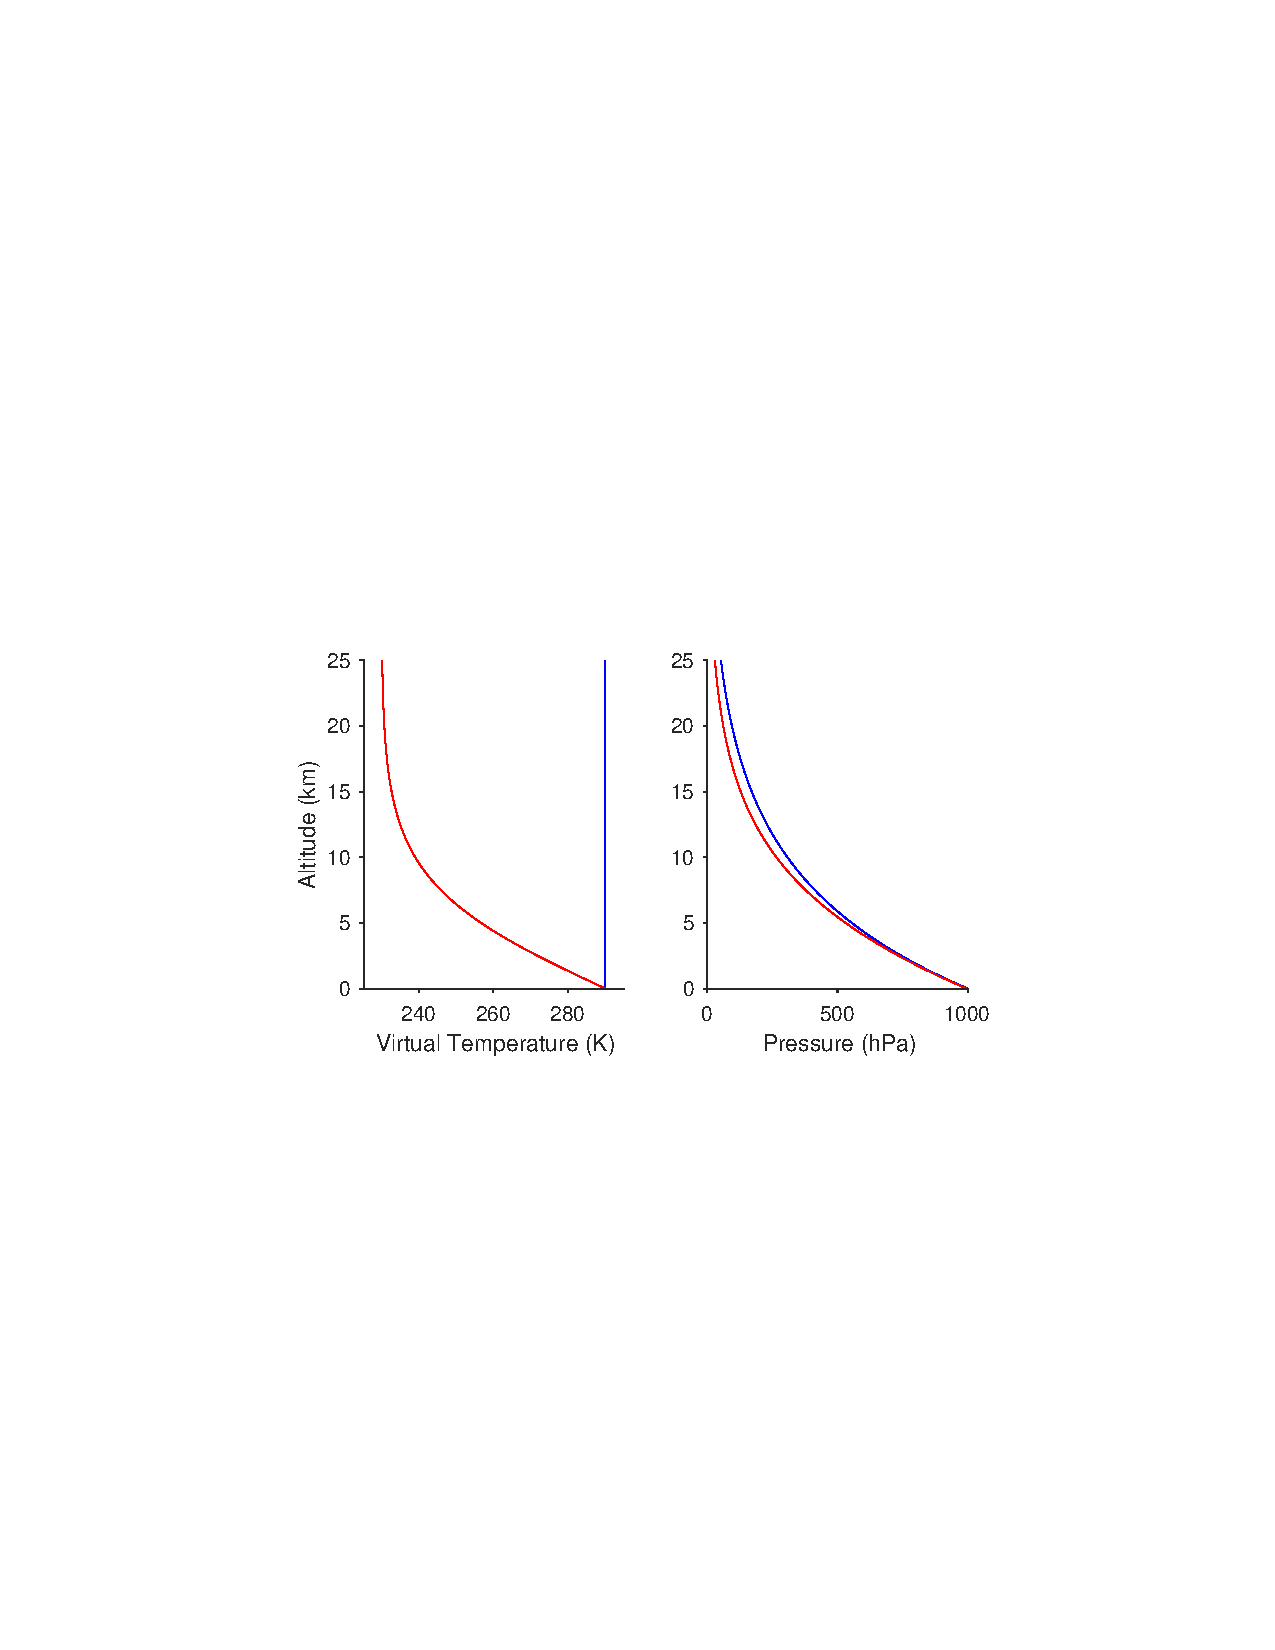
\includegraphics{figures/hydrostatic_state.pdf}
    \caption{(a) An isothermal temperature profile (blue) and a temperature profile \eqref{e:ref_temperature} (red) with surface temperature $T_{\mathrm{sfc}} = 300~\mathrm{K}$, ``stratospheric'' temperature $T_{\min} = 200~\mathrm{K}$, and ``tropospheric'' temperature lapse rate $\Gamma = 6.5~\mathrm{K~km^{-1}}$---values roughly representative of Earth's tropical atmosphere. (b) The corresponding hydrostatically balanced pressure profiles \eqref{eq:hydro_pressure_iso} and \eqref{eq:hydro_pressure_lapse}, with $p_{\mathrm{MSLP}} = 10^5~\mathrm{Pa}$.}
    \label{f:hydrostatic_state}
\end{figure}
The temperature is constant and equal to $T_{\min}$ above $z_t$. See Fig.~\ref{f:hydrostatic_state}a for an example. The resulting temperature profile is a rough approximation of a tropospheric temperature profile with lapse rate $\Gamma$ and a ``tropopause'' at height $z_t$, overlain by a ``stratosphere'' with constant temperature $T_{\min}$. For $\Gamma = g/c_{pd}$, the ``tropospheric'' temperature profile is dry adiabatic. 

\subsubsection{Pressure}

We obtain the pressure $p(z)$ consistent with the temperature profile $T(z)$ by combining hydrostatic balance ($\partial_z p(z) = - \rho g$) with the ideal gas law ($p=\rho R_d T$, neglecting the effect of any moisture on the gas constant), giving
\begin{equation}\label{eq:hydro_pressure}
p(z) = p_{\mathrm{MSLP}} \exp\left(-\int_0^z \frac{dz}{H(z)} \right).
\end{equation}
Here,
\begin{equation}
H(z)  = \frac{R_d T(z)}{g}
\end{equation}
is the scale height, and we chose for the pressure $p(0)$ at height $z=0$ the mean sea-level pressure $p_{\mathrm{MSLP}}$, a model parameter. 

It helps here to distinguish the cases of an isothermal atmosphere and of an atmosphere with nonzero lapse rate:
\begin{itemize}
\item \textbf{Isothermal Atmosphere ($\Gamma = 0$, $T_{\mathrm{sfc}} \ge T_{\min}$).} 
In this case, the pressure becomes 
\begin{equation}\label{eq:hydro_pressure_iso}
    p(z) = p_{\mathrm{MSLP}} \exp \left(-\frac{z}{H_{\mathrm{sfc}}} \right), \qquad H_{\mathrm{sfc}} = \frac{R_d T_{\mathrm{sfc}}}{g} = \mathrm{const}.
\end{equation}
See See Fig.~\ref{f:hydrostatic_state}b (blue line) for an example.

\item \textbf{Nonzero Lapse Rate ($\Gamma \ge 0$, $T_{\mathrm{sfc}} \ge T_{\min}$).}
Integrating the general expression \eqref{eq:hydro_pressure} for the hydrostatic pressure for a temperature profile \eqref{e:ref_temperature} with nonzero lapse rate yields
\begin{equation}\label{eq:hydro_pressure_lapse}
p(z) = p_{\mathrm{MSLP}} \times
\begin{cases}
\left(1 - \frac{\Gamma z}{T_{\mathrm{sfc}}} \right)^{g/(R_d \Gamma)} & \text{for } z \le z_t, \\[1.5ex]
  \left(\frac{T_{\min}}{T_{\mathrm{sfc}}} \right)^{g/(R_d \Gamma)}
 \exp  \left(-\frac{z - z_t}{H_{\min}} \right) & \text{for } z\ge z_t, 
\end{cases}
\end{equation}
where 
\begin{equation}
H_{\min} = \frac{R_d T_{\min}}{g}
\end{equation}
is the ``stratospheric'' scale height. See See Fig.~\ref{f:hydrostatic_state}b (red line) for an example. (The expression \eqref{eq:hydro_pressure_lapse} for nonzero lapse rate converges to the expression \eqref{eq:hydro_pressure_iso} for zero lapse rate in the limit $\Gamma \to 0$, as can be verified by L'H{\^o}pital's rule.)
\end{itemize}

\subsubsection{Density}
 
Given the temperature $T(z)$ and hydrostatic pressure $p(z)$, the reference density $\rho(z)$ follows from the ideal gas law as
\begin{equation}\label{eq:hydro_density}
    \rho(z) = \frac{p(z)}{R_d T(z)}.
\end{equation}

\subsubsection{Specific Humidity}

And the total specific humidity $q_t(z)$ for a given relative humidity, temperature $T(z)$, and density $\rho(z)$ is
\begin{equation}
    q_t(z) = \mathrm{RH} \, q_v^*\bigl( T(z), \rho(z) \bigr),
\end{equation}
where $q_v^*(T, \rho)$ is the saturation specific humidity \eqref{eq:sat_shum}. Corresponding to $\mathrm{RH} < 1$, we set the condensate specific humidities to zero ($q_l = q_i = 0$).

\subsubsection{Energy}

From the above quantities, we can compute the specific internal energy $I$ using Eq.~\eqref{eq:total_internal_energy} and with that the total specific energy $e^{\mathrm{tot}} = I + \Phi$ corresponding to a state of rest ($\vec{u}=0$). This completes the specification of the model state.

\subsubsection{Noise}

It is common to add a small amount of random noise, e.g., to the initial density at the surface, to break the symmetry of the initial state and allow three-dimensional instabilities to develop. A typical standard deviation of such noise may be 1\% of $\rho(0)$.

\section{Abstraction of Model Formulation}\label{s:abstract_model_formulation}

To describe the methods used to solve the governing equations numerically, let us write the equations in the compact form 
\begin{equation}\label{e:eom_compact}
\diff{\vec{Y}}{t}  =  - \nabla \cdot \Fvector + \vec{\mathcal{S}}(\vec{Y}),
\end{equation}
where $\vec{Y}$ is the \emph{state} vector, $\partial\vec{Y}/\partial t$ is the \emph{tendency} of the state vector, $\Fvector$ is the \emph{flux} vector, and $\vec{\mathcal{S}}(\vec{Y})$ are \emph{sources}. 

\subsection{State}

The state vector consists of components
\begin{equation}\label{e:state}
\vec{Y}=\left( \begin{array}{c}
\rho \\
\rho\vec{u} \\
\rho e^{\mathrm{tot}}\\
\rho q_k\\
\rho q_{p,i}\\
\rho \chi_j
\end{array}
\right).
\end{equation}
Here, $q_k$ represents the suspended water specific humidities $q_t$, $q_l$, and/or $q_i$ (total water and cloud condensate, if used); $q_{p,i}$ are the precipitation specific humidities, with the index $i$ labeling different precipitation species (rain, snow, graupel etc.); and $\chi_j$ are the scalar concentrations (e.g., mass of different aerosol species, chemical constituents etc.\ per unit mass of moist air). In some model configurations (e.g., when we include atmospheric chemistry), we may want to have $O(100)$ of these scalars, meaning that the state vector can consist of hundreds of components.

\subsection{Fluxes}\label{sec:fluxes}

The flux $\Fvector=\Fadv + \Pvector +  \Fdiff + \Frad + \Fprecip$ consists of advective fluxes, pressure terms, diffusive fluxes, radiative fluxes, and precipitation fluxes. The diffusive components $\Fdiff$ are proportional to gradients of state variables, so that $\nabla \cdot \Fdiff$ contains elliptic operators. These are treated separately numerically from the non-diffusive fluxes, which do not contain gradients. Because the boundary conditions on advective and other non-diffusive fluxes generally differ, it is also useful to distinguish advective fluxes $\Fadv$, pressure terms $\Pvector$, and the other non-diffusive fluxes due to radiation $\Frad$ and precipitation $\Fprecip$. 

\subsubsection{Advective Fluxes}

The advective flux is generally of the form ``$\rho \times \mathrm{scalar} \times \vec{u}$,'' where $\vec{u}$ is the advective velocity of the working fluid. For the state vector \eqref{e:state}, it is 
 \begin{equation}
 \label{e:adv_flux}
 \Fadv=\rho \left( \begin{array}{c}
 \vec{u} \\
 \vec{u} \otimes \vec{u} \\
 e^{\mathrm{tot}} \vec{u}\\
q_k \vec{u}\\
q_{p,i} \vec{u} \\
\chi_j \vec{u}
\end{array}
\right).
 \end{equation}

\subsubsection{Pressure Terms}

The pressure terms in the momentum and energy equations can also be written in flux form,
\begin{equation}
\Pvector = \left( \begin{array}{c}
\vec{0} \\
p \vec{I}_3 \\
p \vec{u} \\
\vec{0} \\
\vec{0} \\
\vec{0} 
\end{array}
\right).
\end{equation}
Because pressure in a fluid is adjusted by sound waves, which are the fastest modes, the pressure terms are associated with the fastest time scales. 

\subsubsection{Diffusive Fluxes}

 The diffusive component takes the form 
 \begin{equation}
 \Fdiff=\left( \begin{array}{c}
 \rho\vec{d}_{q_t} \\
 \rho\vec{\tau} + \rho\vec{d}_{q_t} \otimes \vec{u}\\
 \vec{u} \cdot \rho\vec{\tau} + \rho (\vec{J} + \vec{D}) \\
\rho\vec{d}_{q_k}\\
\rho \vec{d}_{q_{p, i}}\\
\rho \vec{d}_{\chi_j}
\end{array}
\right).
\label{eq:diff_flux}
\end{equation}
where the water flux $\vec{d}_{q_t}$ is defined in \eqref{eq:sgs-shum-flux}, the momentum flux $\vec{\tau}$ in \eqref{e:sgs_momentum_flux}, the total enthalpy flux $\vec{J} + \vec{D}$ in \eqref{e:SGS_energy_flux}, the fluxes of the water components $\vec{d}_{q_k}$ are defined in \eqref{e:water_diffusion}, the fluxes $\vec{d}_{q_{p, i}}$ of the precipitation components in \eqref{eq:sgs-precip-flux}, and the fluxes $\vec{d}_{\chi_j}$ of tracers in \eqref{eq:sgs-tracer-flux}.


\subsubsection{Other Non-diffusive Fluxes}

The other non-diffusive fluxes include source terms (e.g., radiation) that can be written in flux form but that are not proportional to gradients of state variables, as well as the precipitation fluxes involving the fall velocity $w_p$ (approximately terminal velocity) of falling precipitate:
\begin{equation}
\Frad = 
\left( \begin{array}{c}
\vec{0} \\
\vec{0} \\
\rho \vec{F}_R \\
\vec{0} \\
\vec{0} \\
\vec{0} 
\end{array}
\right), \qquad
\Fprecip = 
\left( \begin{array}{c}
\vec{0} \\
\vec{0} \\
\vec{0} \\
\vec{0} \\
-\rho q_{p,i} w_{p, i} \vec{k} \\
\vec{0} 
\end{array}
\right).
\label{eq:ndf_flux}
\end{equation}
Here, $\vec{k}$ is the vertical unit vector.  The term $-\rho q_{p,i} w_{p, i} \vec{k}$ denotes the falling precipitate flux. (The fall velocity $w_{p, i}$ is a point-wise function of the specific humidity $q_{p,i}$, the environmental density $\rho$, and possibly of other microphysical parameters that determine the size distribution of falling hydrometeors.) The radiative energy flux $\vec{F}_R$ is included here because it is not diffusive in character. In climate models, it generally is approximated as vertical and hence is one-dimensional, like the precipitation flux. Therefore, \emph{the divergence of these two fluxes is a one-dimensional (vertical) divergence}. \hl{[TODO in code: Do we have this implemented as a vertical divergence only?]}

\subsection{Sources}

The right-hand side of the balance law \eqref{e:eom_compact} has the source-sink terms
\begin{multline}
\Source(\vec{Y})= 
 \left( \begin{array}{c}
 -\rho C(q_t \rightarrow q_p) \\
  -\rho \nabla\Phi - 2 \vec{\Omega} \times \rho\vec{u}  + \rho \vec{F}_u \\
 \rho Q - \sum_{j\in\{v,l,i\}} (I_j + \Phi)  \rho C(q_j \rightarrow q_p) + \rho \vec{u} \cdot \vec{F}_u - M \\
\rho C(q_p \rightarrow q_k) + \rho \sum_j \rho C(q_j \rightarrow q_k) \\
\rho \sum_k C(q_k \rightarrow q_{p, i}) - \rho \sum_j C(q_{p, i} \rightarrow q_{p, j})\\
\rho \mathcal{S}_{\chi_i}
\end{array}
\right)
\label{eq:source}
\end{multline}
where $C(q_j \rightarrow q_k)$ represents the conversion of the generic specific humidity $q_j$ to $q_k$ ($k, j \in \{v, l, i\}$), $C(q_p \rightarrow q_k)$ represents the conversion of all precipitation specific humidities $q_p$ to $q_k$, and $C(q_{p, i} \rightarrow q_{p, j})$ represents conversion among precipitation species $q_{p, i}$ and $q_{p, j}$. 

\subsection{Boundary Conditions}

At rigid boundaries with normal $\vec{n}$, the normal component of the advective velocity $\vec{u} \cdot \vec{n}$ vanishes, and so do the normal components of all advective fluxes $\Fadv$. Normal components of diffusive fluxes, on the other hand, generally do not vanish (e.g., there are diffusive energy and momentum fluxes across the lower boundary, as discussed in section~\ref{sct:bc}). For these, Neumann boundary conditions apply. In some circumstances (e.g., simulations with prescribed sea surface temperature), we will also need to specify Dirichlet boundary conditions. 

Thus, generally, we want vanishing normal flux components at rigid boundaries, and Dirichlet conditions on state variables and/or Neumann conditions on diffusive flux components.

\chapter{Numerical Methods}\label{sec:numerical_methods}

\section{Spatial Discretization}

\hl{2019/09/19: I (Jeremy) am working on rewriting this section. Still have some
things to add, so it should be seen as a work in progress\dots}

\subsection{Overview}
For the spatial discretization, we use variants of the discontinuous Galerkin
(DG) method with tensor-product bases (see, e.g., \citealt{giraldo:2008a,
abdi:2016}). We use hexahedral (cube) elements in three dimensions.  The nodal
tensor-product DG methods are extremely accurate and efficient.  For example,
using a basis comprised of $N$-th degree Lagrange polynomials results in
approximately an accuracy of $\order(\Delta x^{N+1})$. Furthermore, using
inexact integration results in a per-element complexity of $\order(N^{d+1})$ for
constructing derivatives, where $d$ denotes the dimension of the space. For both
the global and LES models, we use fully three-dimensional DG methods.

The domain is assumed to be embedded in a Cartesian
coordinate system. The vector $\vec{x}$ denotes a point in the Cartesian
coordinate system with components $(x_{1}, x_{2},
x_{3})$. Each element has its own reference coordinate system, defined
so that the element is a square (in 2D) or cube (in
3D). A point in the reference element is denoted as $\vec{\xi}$ with components
$(\xi_{1}, \xi_{2}, \xi_{3})$.  It is important to note that $x_{3} \ne z$ if
$z$ is taken to be height (the direction opposite to the gravitational
acceleration).

\subsection{Balance Law Formulation}
We are interested in solving balance laws in $d$ dimensions of the form
\begin{align}
  &\diff{\vec{Y}}{t} + \nabla \cdot \Fnondiff + \nabla \cdot \Fdiff
  =
  \Source,\\
  &\vec{\Sigma} = \diffusive(\vec{Y}, \nabla \gradvariables(\vec{Y}, \vec{x}, t), t).
\end{align}
Here, $\vec{Y}$ is the state vector, $\Source$ are the sources, and
$\Fnondiff$ and $\Fdiff$ are components of the flux function, namely the
non-diffusive and diffusive flux terms. The flux functions are taken to have the
following form
\begin{align}
  \Fnondiff &= \Fnondiff\left(\vec{Y}, \vec{x}, t\right),\\
  \Fdiff &= \Fdiff\left(\vec{Y}, \vec{\Sigma}, \vec{x}, t\right).
\end{align}
In terms of the fluxes introduced in Sec.~\ref{sec:fluxes}, the non-diffusive
flux is $\Fnondiff = \Fvector - \Fdiff$.

The variable $\vec{\Sigma}$ is an auxiliary variable that has been introduced to
account for terms that depend on the gradient of $\vec{Y}$. The function
$\gradvariables$ transforms the state prior to the variables to have the
gradient taken and the function $\diffusive$ is used to transform to the
auxiliary variables. In principle $\diffusive$ could be applied in $\Fdiff$ but
this formulation allows the most flexibility in terms of enforcing continuity of
the solution, namely $\vec{\Sigma}$ should be the quantity that continuity is
enforced on.

Currently, in the CLIMA source\footnote{see
\texttt{src/DGmethods/balanacelaw.jl} at
\url{https://github.com/climate-machine/CLIMA/blob/master/src/DGmethods/balancelaw.jl}}
the above functions are defined as

\begin{table}[h]
  \centering
  \begin{tabular}{ll}
    $\Fnondiff$       & \texttt{flux\_nondiffusive!}\\
    $\Fdiff$          & \texttt{flux\_diffusive!}\\
    $\gradvariables$  & \texttt{gradvariables!!}\\
    $\diffusive$      & \texttt{diffusive!}\\
    $\Source$         & \texttt{source!}\\
  \end{tabular}
\end{table}

\subsection{Finite Element Mesh}
In finite element methods, the domain is decomposed into a set of elements and
the solution is approximated in each element using a finite dimensional function
space. The solution approximation is constructed by requiring that the residual
is orthogonal (in some inner product) to the space of functions. In the
discontinuous Galerkin method, the choice of numerical method for CLIMA,
the space of functions is discontinuous across element boundaries as continuity
of the solution and boundary conditions are enforced weakly through the use of
numerical fluxes (similar to finite volume methods).

As is often done in finite elements, elements are mapped to a reference domain.
In the reference domain the elements have the domain ${[-1, 1]}^d$ where $d$ is
the dimensionality of the problem; thus in 2-D the reference element is a square
and in 3-D a cube. There is then a diffeomorphic mapping between each element in
the physical space and the reference space. Thus, for a single element $e$ the
mapping is of the form $\vec{x}^{(e)}(\vec{\xi})$ and its inverse is
$\vec{\xi}^{(e)}(\vec{x})$; note that each element will have a different mapping
function. These mapping must be accounted for when discretizing the equations
through the use of metric terms.

\subsection{Basis Functions}
On the reference element, the space of functions used is tensor-product
polynomials of degree $N$; the space of tensor-product polynomials of degree $N$
is denoted as $\mathbb{Q}^{N}(\hat{e})$ where $\hat{e} = {[-1, 1]}^d$ is the
reference element. In 3-D the solution inside the element is taken to be
\begin{align}
  \vec{Y}^{(e)}(\vec{\xi}, t) = \sum_{(i,j,k) = (0,0,0)}^{(N,N,N)}
  l_{i}(\xi_{1}) l_{j}(\xi_{2}) l_{k}(\xi_{3})
  \vec{Y}_{ijk}^{(e)}(t),
\end{align}
Here $l_{i}(\vec{x})$ are 1-D Lagrange polynomials associate with a set of
abscissae ${\{\hat{\xi}_{k}\}}_{k=0}^{N}$ (which should not be confused with
$\xi_{k}$ which is a component of $\vec{\xi}$). In terms of the physical
coordinate $\vec{x}$ the solution inside the element is then
\begin{align}
  \vec{Y}^{(e)}(\vec{\xi}^{(e)}(\vec{x}), t) = \sum_{(i,j,k) = (0,0,0)}^{(N,N,N)}
  l_{i}(\xi_{1}^{(e)}(\vec{x})) l_{j}(\xi_{2}^{(e)}(\vec{x}))
  l_{k}(\xi_{3}^{(e)}(\vec{x}))
  \vec{Y}_{ijk}^{(e)}(t).
\end{align}
Note that depending on the mapping $\vec{\xi}^{(e)}(\vec{x})$ the solution need
not be tensor product polynomial in the physical space.

\subsection{DG Formulation}
The discontinuous Galerkin scheme used in CLIMA is: for element $e$ find a
function $\vec{Y}^{(e)} \in \mathbb{Q}^{N}(\hat{e})$
and $\vec{\Sigma}^{(e)} \in \mathbb{Q}^{N}(\hat{e})$
such that
\begin{align}
  &\int_{e}
  \left(
  \vec{\Psi}^T \diff{\vec{Y}}{t}
  + \frac{1}{2}
  \left(
  \vec{\Psi}^{T} \nabla \cdot \Fnondiff
  -
  \nabla\vec{\Psi} \cdot
  \Fnondiff
  \right)
  -
  \nabla\vec{\Psi} \cdot
  \Fdiff
  \right)\\\notag
  &\quad\quad\quad =
  \int_{e} \vec{\Psi}^T \Source
  -
  \int_{\partial e}
  \vec{\Psi}^{T}
  {\left(\nhat^{-} \cdot \Fdiff\right)}^{*}
  \\\notag
  &\quad\quad\quad\phantom{=}-
  \int_{\partial e}
  \vec{\Psi}^{T} \left(
  {\left(\nhat^{-} \cdot \Fnondiff\right)}^{*}
  - \frac{1}{2} \nhat^{-} \cdot {\left(\Fnondiff\right)}^{-}
  \right)
  ,\\
  &\int_{e}
  \left(
  \vec{\Phi}^T \vec{\Sigma}
  -
  \vec{\Phi}^T \diffusive(\vec{Y}, \nabla \gradvariables, t)
  \right)
  =
  \int_{\partial e} \vec{\Phi}^{T} \left(
  \diffusive^{*} - \diffusive\left(\vec{Y}^{-},
  \nhat^{-}\gradvariables^{-}, t\right)
  \right),
\end{align}
for all $\vec{\Psi} \in \mathbb{Q}^{N}(\hat{e})$ and $\vec{\Phi} \in
\mathbb{Q}^{N}(\hat{e})$.  Here it is understood that $\Fnondiff =
\Fnondiff(\vec{Y}, t)$, $\Fdiff = \Fdiff(\vec{Y}, \vec{\Sigma}, t)$, and
$\gradvariables = \gradvariables(\vec{Y}, t)$. In the surface integrals, the
terms with a subscript $-$ are evaluated inside the element and the terms with a
subscript $*$ are the numerical fluxes which enforce continuity of the solution
across element interfaces and are used to enforce boundary conditions. At
interior element interfaces the numerical flux functions have the following
dependencies:
\begin{align}
  {\left(\nhat^{-} \cdot \Fnondiff\right)}^{*}
  &=
  {\left(\nhat^{-} \cdot \Fnondiff\right)}^{*}
  \left(
  \vec{Y}^{-}, \vec{Y}^{+}, \nhat^{-}, t
  \right),\\
  %
  {\left(\nhat^{-} \cdot \Fdiff\right)}^{*}
  &=
  {\left(\nhat^{-} \cdot \Fdiff\right)}^{*}
  \left(
  \vec{Y}^{-}, \vec{Y}^{+}, \vec{\Sigma}^{-}, \vec{\Sigma}^{+}, \nhat^{-}, t
  \right),\\
  %
  \diffusive^{*} &=
  \diffusive^{*}\left(
  \vec{Y}^{-}, \vec{Y}^{+}, \nhat^{-}, t
  \right).
\end{align}
The numerical fluxes are implemented in the CLIMA
source\footnote{see
\texttt{src/DGmethods/NumericalFluxes.jl} at
\url{https://github.com/climate-machine/CLIMA/blob/master/src/DGmethods/NumericalFluxes.jl}}
in the following functions:

\begin{table}[h]
  \centering
  \begin{tabular}{cl}
    ${\left(\nhat^{-} \cdot \Fnondiff\right)}^{*}$ & \texttt{numerical\_flux\_nondiffusive!}\\
    ${\left(\nhat^{-} \cdot \Fdiff\right)}^{*}$    & \texttt{numerical\_flux\_diffusive!}\\
    $\diffusive^{*}$                               & \texttt{numerical\_flux\_gradient!}\\
  \end{tabular}
\end{table}

\subsection{Numerical Flux}
A variety of choices can be made for the numerical flux functions, and here we
outline the choices made by \citet{bassi:1997nse} which we currently follow
in CLIMA\@.

The numerical flux for the non-diffusive flux\footnote{In \citet[Eq.
(10)]{bassi:1997nse} this is the function $\vec{h_{e}}$.} is set using the
Rusanov (or Local Lax-Friedrichs) flux:
\begin{align}
  {\left(
  \nhat^{-} \cdot \Fnondiff\right)}^{*} =
  \frac{\nhat^{-} \cdot \left(
  {\left(\Fnondiff\right)}^{-} +
  {\left(\Fnondiff\right)}^{+}\right)
  +
  \lambda
  \left(
  \vec{Y}^{-}
  -
  \vec{Y}^{+}
  \right)}{2},
\end{align}
where $\lambda = \lambda(\vec{Y}^{-}, \vec{Y}^{+})$ is an estimate of the
maximum wavespeed, i.e., the maximum eigenvalue of the Jacobian of the flux
function $\Fnondiff$. Here the subscript $+$ denotes the value on face of the
opposing element. As noted in \citet{bassi:1997nse} other choices of the
non-diffusive numerical flux are possible such as Roe, Engquist-Osher, HLLE
(Harten, Lax, Van Leer, Einfeldt), and exact Godunov.

The numerical flux for the diffusive flux\footnote{In \citet[Eq.
(15)]{bassi:1997nse} this is the function $\vec{h_{v}}$.} is set using the
central flux:
\begin{align}
  {\left(
  \nhat^{-} \cdot \Fdiff\right)}^{*} =
  \frac{\nhat^{-} \cdot \left(
  {\left(\Fdiff\right)}^{-} + {\left(\Fdiff\right)}^{+}
  \right)}{2}.
\end{align}

The numerical flux for the auxiliary equation\footnote{In \citet[Eq.
(13)]{bassi:1997nse} this is the function $\vec{H_{s}}$.} is set using the
central flux:
\begin{align}
  \diffusive^{*} = \frac{ \diffusive^{-} + \diffusive^{+} }{2}.
\end{align}

\subsection{Boundary Conditions}
For faces on the boundary of the domain the numerical fluxes are set so that the
boundary condition is enforced weakly. Currently, in CLIMA this is done by
calling the same numerical flux functions except with the exterior (or ghost)
states $\vec{Y}^{+}$ and $\vec{\Sigma}^{+}$ set based on the interior state
$\vec{Y}^{-}$ and $\vec{\Sigma}^{-}$ and boundary condition type. For all three
numerical fluxes this is done with the function \texttt{boundary\_state!} with
multiple dispatch used to distinguish between the different fluxes\footnote{see
\texttt{src/DGmethods/NumericalFluxes.jl} at
\url{https://github.com/climate-machine/CLIMA/blob/master/src/DGmethods/NumericalFluxes.jl}}.

Generally speaking, there is no generic way to do this for all boundary
conditions and each boundary condition must be handled separately. Following,
\citet{bassi:1997nse} here a few different boundary treatments are outlined for
compressible Navier-Stokes. In this case we take the state vector $\vec{Y}$} and
diffusive variables $\vec{\Sigma}$ to be
\begin{align}
  \vec{Y} &=
  \begin{pmatrix}
    \rho\\
    \rho\vec{u}\\
    \rho e^{\rm tot}
  \end{pmatrix},
  &
  \vec{\Sigma} &= \rho \vec{\tau}
\end{align}

\subsubsection{Inflow and Outflow Boundary Conditions}
The inflow and outflow boundary condition for compressible Navier-Stokes says
that $\vec{Y} = \vec{Y}^{\rm bc}$ is known on the boundary. To enforce this, in the
non-diffusive and diffusive numerical $\vec{Y}^{+} = \vec{Y}^{\rm bc}$ is set and in
the diffusive numerical flux $\vec{S}^{+} = \vec{S}^{-}$. In the gradient
numerical flux, $\vec{Y}^{+} = 2\vec{Y}^{\rm bc} - \vec{Y}^{-}$ so that
$\diffusive^{*} = \diffusive^{\rm bc}$ after the central flux has been applied.
This is summarized as:
\begin{align}
  {\left( \nhat^{-} \cdot \Fnondiff\right)}^{*} &=
  {\left( \nhat^{-} \cdot \Fnondiff\right)}^{*}
  \left(\vec{Y}^{-}, \vec{Y}^{\rm bc}, \nhat^{-}, t\right),\\
  {\left( \nhat^{-} \cdot \Fdiff\right)}^{*} &=
  {\left( \nhat^{-} \cdot \Fdiff\right)}^{*}
  \left(\vec{Y}^{-}, \vec{Y}^{\rm bc}, \vec{\Sigma}^{-}, \vec{\Sigma}^{-},
  \nhat^{-}, t\right),\\
  \diffusive^{*} &=
  \diffusive^{*}
  \left(\vec{Y}^{-}, 2\vec{Y}^{\rm bc}-\vec{Y}^{-}, \nhat^{-}, t\right).
\end{align}

\subsubsection{No Flux / Flow Boundary Conditions}
In no flux/flow boundary conditions, the condition to enforce is that $\nhat
\cdot \vec{u} = 0$ along with either
\begin{enumerate*}[label = (\roman*)]
  \item no boundary condition on $\vec{\Sigma}$; or
  \item $\vec{\Sigma} = \vec{\Sigma}^{\rm bc}(\vec{Y}, t)$.
\end{enumerate*}
To enforce these conditions it is convenient define
\begin{align}
  \vec{Y}^{\rm bc}
  =
  \begin{pmatrix}
    \rho^{-}\\
    \left(\vec{I} - 2 \nhat^{-} {\left(\nhat^{-}\right)}^{T}\right)
    {\left(\rho \vec{u}\right)}^{-}\\
    {\left(\rho e^{\rm tot}\right)}^{-}
  \end{pmatrix}.
\end{align}
Importantly since the momentum component is just a Householder reflection of the
${\left(\rho \vec{u}\right)}^{-}$ across the plane defined by $\nhat^{-}$, the
norm is preserved, in particular $\|\vec{u}^{-}\|_{2} = \|\vec{u}^{\rm
bc}\|_{2}$. This means that pressure computed from $\vec{Y}^{-}$ and
$\vec{Y}^{\rm bc}$ will be the same. Additionally, when $\vec{u}^{-}$ and
$\vec{u}^{\rm bc}$ are averaged the result has no normal component:
\begin{align}
  \frac{1}{2}\nhat\cdot\left(\vec{u}^{-} + \vec{u}^{\rm bc}\right) = 0,
\end{align}
which is the desired boundary condition (other component are not modified
including the tangential velocity).

For the non-diffusive and diffusive fluxes, the exterior state is set as
$\vec{Y}^{+} = \vec{Y}^{\rm bc}$ and in the gradient transform
$\vec{Y}^{+} = 2\vec{Y}^{\rm bc} - \vec{Y}^{-}$; this is the same as in the
inflow/outflow case after setting $\vec{Y}^{\rm bc}$ as above.

In the case of no boundary condition on $\vec{\Sigma}$ the exterior value is set
as $\vec{\Sigma}^{+} = \vec{\Sigma}^{-}$ and the numerical fluxes are:
\begin{align}
  {\left( \nhat^{-} \cdot \Fnondiff\right)}^{*} &=
  {\left( \nhat^{-} \cdot \Fnondiff\right)}^{*}
  \left(\vec{Y}^{-}, \vec{Y}^{\rm bc}, \nhat^{-}, t\right),\\
  {\left( \nhat^{-} \cdot \Fdiff\right)}^{*} &=
  {\left( \nhat^{-} \cdot \Fdiff\right)}^{*}
  \left(\vec{Y}^{-}, \vec{Y}^{\rm bc}, \vec{\Sigma}^{-}, \vec{\Sigma}^{-},
  \nhat^{-}, t\right),\\
  \diffusive^{*} &=
  \diffusive^{*}
  \left(\vec{Y}^{-}, 2\vec{Y}^{\rm bc}-\vec{Y}^{-}, \nhat^{-}, t\right).
\end{align}

In the case of a boundary condition on $\vec{\Sigma}$ the exterior value is set
as $\vec{\Sigma}^{+} = \vec{\Sigma}^{\rm bc}\left(\vec{Y}^{\rm bc}, t\right)$
and the numerical fluxes are:
\begin{align}
  {\left( \nhat^{-} \cdot \Fnondiff\right)}^{*} &=
  {\left( \nhat^{-} \cdot \Fnondiff\right)}^{*}
  \left(\vec{Y}^{-}, \vec{Y}^{\rm bc}, \nhat^{-}, t\right),\\
  {\left( \nhat^{-} \cdot \Fdiff\right)}^{*} &=
  {\left( \nhat^{-} \cdot \Fdiff\right)}^{*}
  \left(\vec{Y}^{-}, \vec{Y}^{\rm bc}, \vec{\Sigma}^{-}, \vec{\Sigma}^{\rm bc}
  \left(\vec{Y}^{\rm bc}, t\right),
  \nhat^{-}, t\right),\\
  \diffusive^{*} &=
  \diffusive^{*}
  \left(\vec{Y}^{-}, 2\vec{Y}^{\rm bc}-\vec{Y}^{-}, \nhat^{-}, t\right).
\end{align}
\hl{Should $\vec{Y}^{\rm bc}$, $\vec{Y}^{\rm -}$, or an average be used here?
--- Jeremy}

\subsubsection{No Slip Conditions}
In no slip boundary conditions, the condition to enforce is that $\vec{u} =
\vec{0}$ along with either
\begin{enumerate*}[label = (\roman*)]
  \item no boundary condition on $\vec{\Sigma}$; or
  \item $\vec{\Sigma} = \vec{\Sigma}^{\rm bc}(\vec{Y}, t)$.
\end{enumerate*}
To enforce these conditions it is convenient define
\begin{align}
  \vec{Y}^{\rm bc}
  =
  \begin{pmatrix}
    \rho^{-}\\
    -{\left(\rho \vec{u}\right)}^{-}\\
    {\left(\rho e^{\rm tot}\right)}^{-}
  \end{pmatrix}.
\end{align}
As in the no flux / flow case, the norm is preserved and the pressure is
preserved.  Additionally, when $\vec{u}^{-}$ and
$\vec{u}^{\rm bc}$ are averaged the result is a zero velocity,
which is the desired boundary condition (other component are not modified).

The remainder of the implementation is the same as in the no flux / flow case.

\subsection{Implementation Details (aka Quadrature and Variational Crimes)}
\hl{FILL ME\@!}

\subsection{Energy Analysis of Advection-Diffusion}
\hl{FILL ME\@!}

\hl{Still TODO\@:}
\begin{itemize}
  \item Bring code in line with skew symmetric formulation
  \item Replace in code \texttt{diffusive\_penalty!} with
    \texttt{gradient\_numerical\_flux!}
  \item Check / correct boundary conditions already in use in the code
  \item Add more BC types?
  \item Add details on BCs for moisture / tracer variables
  \item Add DG refs (skew symmetric formulation stuff, geometry handling, etc.)
\end{itemize}

\section{Time-Discretization Methods}\label{s:timestepping}

The general, compressible equations of motion we use permit a variety of wave modes with different characteristic speeds. Additionally, the equations contain sources that can add stiffness, for example, from microphysical processes that occur on timescales of seconds or less.

The equations permit the following wave modes:
\begin{itemize}
    \item Acoustic waves. They have phase speeds (Eq.~\eqref{e:soundspeed}) around $300~\mathrm{m~s^{-1}}$. Density variations and the terms involving pressure in the momentum and energy equations are essential for their existence.
    \item Gravity waves. They have a spectrum of phase speeds. In a deep atmosphere (e.g., in a GCM), the gravest, external mode has phase speed $(gH)^{1/2} \approx 280~\mathrm{m~s^{-1}}$, where $H\approx 8~\mathrm{km}$ is the atmospheric scale height. The gravity term $-\rho \nabla \Phi$ in the momentum equation and the gravitational potential energy $\Phi$ in the energy equation are responsible for their existence.
    \item Inertia-gravity, Rossby waves, and several other wave modes that owe their existence to the Coriolis acceleration $-2\vec{\Omega} \times \rho \vec{u}$. They have smaller phase speeds than the acoustic and external gravity waves.
\end{itemize}
Additional stiffness in the equations arises from:
\begin{itemize}
    \item Falling precipitation, whose fall velocity $w_{p,i}$ can reach $10~\mathrm{m~s^{-1}}$ and thus exceeds typical vertical velocities resolved in GCMs.
    \item Microphysical source terms, for example, in the equations for suspended specific humidities $q_k$; they depend on the precipitation specific humidity $q_{p,i}$, which can change rapidly because precipitate falls rapidly. 
    \item SGS diffusive fluxes, whose effective vertical velocity can exceed that of the resolved velocities.
    \item Other parameterized SGS fluxes, for example, convective updrafts, whose vertical velocities can likewise be large.
\end{itemize}
By contrast, radiation evolves on longer timescales than the dynamical quantities and hence, because it is expensive to evaluate, usually is evolved forward in time with longer timesteps than the dynamical quantities. 

Hence, we need a stable and computationally efficient time discretization strategy that allows some state vector components to be subcycled several times per dynamical timestep (e.g., $q_{p,i}$ and convective updrafts) and allows some rapidly evolving source/sink terms (e.g., from microphysics) to be accumulated over the subcycled timesteps. At the same time, it should allow other terms (e.g., radiative energy fluxes) to be evaluated less frequently. In particular, we need a computationally efficient way of handling the physically insignificant acoustic waves.

\subsection{Additive Runge-Kutta IMEX Methods}

To circumvent the time-step restriction due to the fast acoustic and gravity waves, using implicit-explicit (IMEX) methods is one option. For the LES model, if the aspect ratio of the horizontal ($\Delta_h$) to vertical ($\Delta_v$) grid spacing is near unity, it may be beneficial to use fully 3D-IMEX methods.  For LES models with aspect ratios of grid elements $\Delta_h/\Delta_v > 1$ and for global atmospheric models, which generally have $\Delta_h/\Delta_v \gg 1$, we use 1D-IMEX methods in which the time-integrator is fully explicit in the horizontal direction (HE) and implicit in the vertical direction (so-called HEVI schemes). 

IMEX methods require the solution of one or more linear systems at each time step. The linear system is global in 3D, and this may limit scalability of IMEX methods in a multi-node computational setting. In that case, split-explicit methods may be a more scalable option to deal with the timestep restrictions. For HEVI schemes, the linear solves are restricted to independent atmospheric columns, which are usually represented on a single compute node (if the domain decomposition is done in the horizontal). So their scalability across nodes is less restricted.

We use a general family of additive Runge-Kutta methods (ARK) methods for 1D and 3D IMEX approaches (see, e.g., \citet{giraldo:2013}). Note that the same infrastructure of the linear (implicit) and nonlinear (explicit) decomposition can also be used in the substepping (e.g., split-explicit) approach.

To get a sense of how the ARK approach works, let us describe a general abstract model here that will be used in later sections to describe specific formulations. To illustrate the abstract IMEX formulation, let us partition the total tendency $\vec{\mathcal{T}}$ on the right-hand side of Eq.~\eqref{e:eom_compact} into four terms: 
\begin{itemize}
    \item terms to be treated implicitly, labeled by $I$ (the fastest terms);
    \item terms evaluated at the dynamical (advective) timestep, labeled by $d$;
    \item terms to be subcycled $f$ times for each dynamical timestep, labeled by $+f$ (for fast);
    \item terms to be evaluated every $s$ dynamical timesteps, labeled by $-s$ (for slow).
\end{itemize}
This gives
\[
\frac{\partial \vec{Y}}{\partial t} = \Tvector = - \nabla \cdot \Fvector + \vec{\mathcal{S}} = \Tvector_{I} + \Tvector_{d} + \Tvector_{+f} + \Tvector_{-s}.
\]
To obtain a linear problem for the implicit solve, let us linearize the implicit tendency terms $\Tvector_{I}$ by Taylor expansion around a reference state $\vec{Y}_r$,
\begin{equation}\label{e:imex_linearization}
\Tvector_{I}(\vec{Y}) =  \Tvector_I(\vec{Y}_r) + \vec{\mathcal{L}}_I (\vec{Y} - \vec{Y}_r) + \Tvector^N_{I}(\vec{Y}),
\end{equation}
where 
\begin{equation}
    \vec{\mathcal{L}}_I = \left. \frac{\partial\Tvector_I}{\partial\vec{Y}}\right|_{\vec{Y}_r}
\end{equation} 
is the linear component of the tendency operator and $\Tvector^N_{I}(\vec{Y})$ is the nonlinear residual. This then allows us to write the equation of motion \eqref{e:eom_compact} as
\begin{equation}
\label{eq:IMEX}
\frac{\partial\vec{Y}}{\partial t} =  \vec{\mathcal{L}}_I \vec{Y} + \Bigl(\Tvector_I(\vec{Y}_r) - \vec{\mathcal{L}}_I \vec{Y}_r\Bigr) + \Tvector^N_{I}(\vec{Y}) + \Tvector_{d} + \Tvector_{+f} + \Tvector_{-s}.
\end{equation}
Usually, the reference state $\vec{Y}_r$ is chosen so that the tendency of the reference state, $\Tvector_I(\vec{Y}_r)$, and the linear tendency of the reference state, $\vec{\mathcal{L}}_I \vec{Y}_r$, either vanish individually or cancel each other, so that $\Tvector_I(\vec{Y}_r) - \vec{\mathcal{L}}_I \vec{Y}_r=0$. We will assume that in what follows and justify it in section~\ref{s:IMEX_general}.

Assuming that $\Tvector_I(\vec{Y}_r) - \vec{\mathcal{L}}_I \vec{Y}_r=0$, let us
describe the 3D-IMEX approach, by focusing on the simpler form of Eq.\ \eqref{eq:IMEX} without the fast term $\Tvector_{+f}$: 
\begin{equation}
\label{eq:IMEX_v2}
\frac{\partial\vec{Y}}{\partial t} =  \vec{\mathcal{L}}_I \vec{Y} + \Tvector^N_{I} + \Tvector_{d} + \Tvector_{-s}.
\end{equation}
We rewrite this as
\begin{equation}
\label{eq:IMEX_v3}
\frac{\partial\vec{Y}}{\partial t} =  \vec{\mathcal{L}}_I \vec{Y} + \Tvector_{p} + \Tvector_{-s}
\end{equation}
where $\Tvector_{p}=\Tvector^N_{I} + \Tvector_{d}$ capture the ``physical'' mode (subscript $p$), for lack of a better term (is what Wicker and Skamarock call this mode - \textbf{need reference} \hl{[dynamical mode of something like it would be better--this is not what people usually call 'physics']}).
\begin{algorithm}
\label{alg:3d-imex_v1}
\begin{algorithmic}
\State
\Function{3D-IMEX with Superstepping}{}
\For{$i=1:S$} 
\State $\left( \vec{I} - \Delta t \widetilde{a}_{ii} \vec{\mathcal{L}}_I \right) \vec{Y}^{(i)}=\vec{Y}^{n} + \Delta t \sum_{j=1}^{i-1} \left( a_{ij} \Tvector_{p}(\vec{Y}^{(j)}) + a_{ij} \Tvector_{-s}(\red{\vec{Y}^{n-s}})
+ \widetilde{a}_{ij} \vec{\mathcal{L}}_I \vec{Y}^{(j)} \right)$ 
\EndFor %i
\State $\vec{Y}^{n+1}=\vec{Y}^{n} + \Delta t \sum_{i=1}^{S} b_{i} \left[ \Tvector_{p}(\vec{Y}^{(i)}) + \Tvector_{-s}(\red{\vec{Y}^{n-s}})
+ \vec{\mathcal{L}}_I \vec{Y}^{(i)} \right]$
\EndFunction
\end{algorithmic}
\end{algorithm}
In Alg.\ \ref{alg:3d-imex_v1}, the fastest waves (e.g., acoustic and gravity waves) are solved implicitly for each stage $i$ of the RK method with $S$-stages, the term $\red{\vec{Y}^{n-s}}$ is frozen at the time level $n-s$, and $a_{ij}$, $\widetilde{a}_{ij}$, and $b_i$ are the RK coefficients in Butcher tableau form (see Table \ref{eq:butcher_tableau}) and therefore represents a general formulation.
\begin{equation}
\begin{array}{c|c}
\ST c&A\\
\hline
\ST  & b\transpose
\end{array}
\hspace{0.5in}
\begin{array}{c|c}
\ST \wt{c} & \wt{A} \\
\hline
\ST  & \wt{b} \transpose
\end{array}
\label{eq:butcher_tableau}
\end{equation}
Here, $A=a_{ij}, \; i,j=1,\ldots S$, and $c_i=\sum_{j} a_{ij}$ represent the time when the right-hand side is evaluated; that is, we evaluate it at each stage which occurs at the time interval $t+c_i \dt$.
In addition, $b=\wt{b}$ is necessary in order to conserve all linear invariants \cite{giraldo:2013}.

If we now include the medium-fast terms denoted by $\Tvector_{+f}$ then we can modify Alg.\ \ref{alg:3d-imex_v1} as summarized in Alg.\ \ref{alg:3d-imex_v2} where for simplicity we assume a 3-partition IMEX multirate strategy based on Euler's method.
\begin{algorithm}
\label{alg:3d-imex_v2}
\begin{algorithmic}
\State
\Function{3D-IMEX Multirate with 3-Partitions based on Euler's Method}{}
\State $\vec{Y}^{(0)}=\vec{Y}^{n}$
\For{$m=1:M$} 
\State $\vec{Y}^{(m)}=\vec{Y}^{(m-1)} + \frac{\Delta t}{M} \Tvector_{+f}(\vec{Y}^{(m)})$
\EndFor %m
\State $\left( \vec{I} - \Delta t \vec{\mathcal{L}}_I \right) \vec{Y}^{(M)}=\vec{Y}^{(m)}$
\State $\vec{Y}^{n+1}=\vec{Y}^{n} + \Delta t \left[ \Tvector_{-s}(\red{\vec{Y}^{n-s}}) + \Tvector_{p}(\vec{Y}^{(M)}) + 
\Tvector_{+f}(\vec{Y}^{(M)}) + 
\vec{\mathcal{L}}_I \vec{Y}^{(M)} \right]$
\EndFunction
\end{algorithmic}
\end{algorithm}
A more general form of Alg.\ \ref{alg:3d-imex_v2} can be found in Alg.\ \ref{alg:3d-imex_v3} where we now replace the outside Euler loop with an I-stage Additive Runge-Kutta method. 
\begin{algorithm}
\label{alg:3d-imex_v3}
\begin{algorithmic}
\State
\Function{3D-IMEX Multirate with 3-Partitions based on ARK and Euler's Method}{}
\State $\vec{Y}^{(i)}=\vec{Y}^{n}$
\For{$i=2:I$} 
\State $\vec{Y}^{(0)}=\vec{Y}^{(i)}$
\For{$m=1:M$} 
\State $\vec{Y}^{(m)}=\vec{Y}^{(m-1)} + \frac{\left(c_i - c_{i-1} \right) \Delta t}{M} \Tvector_{+f}(\vec{Y}^{(m)})$
\EndFor %m
\State $\left( \vec{I} - \Delta t \widetilde{a}_{ii} \vec{\mathcal{L}}_I \right) \vec{Y}^{(i)}=\vec{Y}^{(m)} + \Delta t \sum_{j=1}^{i-1} \left( a_{ij} \Tvector_{p}(\vec{Y}^{(j)}) + \widetilde{a}_{ij} \vec{\mathcal{L}}_I \vec{Y}^{(j)} \right)$
\EndFor %i
\State $\vec{Y}^{n+1}=\vec{Y}^{n} + \Delta t \sum_{j=1}^{i} b_i \left[ \Tvector_{-s}(\red{\vec{Y}^{n-s}}) + \Tvector_{p}(\vec{Y}^{(i)}) + 
\Tvector_{+f}(\vec{Y}^{(i)}) + 
\vec{\mathcal{L}}_I \vec{Y}^{(i)} \right]$
\EndFunction
\end{algorithmic}
\end{algorithm}

A slightly more general form of Alg.\ \ref{alg:3d-imex_v3} can be found in Alg.\ \ref{alg:3d-imex_v4} where we now replace the inner Euler loop with an J-stage explicit Runge-Kutta method. 
\begin{algorithm}
\label{alg:3d-imex_v4}
\begin{algorithmic}
\State
\Function{3D-IMEX Multirate with 3-Partitions based on ARK}{}
\State $\vec{Y}_i^{(i)}=\vec{Y}^{n}$
\For{$i=2:I$} 
\State $\vec{Y}_j^{(1)}=\vec{Y}_i^{(i)}$
\For{$j=2:J$} 
\State $\vec{Y}_j^{(j)}=\vec{Y}_i^{(i-1)} + \left(c_i - c_{i-1} \right) \Delta t \sum_{k=1}^{j-1} a_{jk} \Tvector_{+f}(\vec{Y}_j^{(k)})$
\EndFor %j
\State $\vec{Y}^{(*)}=\vec{Y}_i^{(i-1)} + \left(c_i - c_{i-1} \right) \Delta t \sum_{j=1}^{J} b_j \Tvector_{+f}(\vec{Y}_j^{(j)})$
\State $\left( \vec{I} - \Delta t \widetilde{a}_{ii} \vec{\mathcal{L}}_I \right) \vec{Y}_i^{(i)}=\vec{Y}^{(*)} + \Delta t \sum_{j=1}^{i-1} \left( a_{ij} \Tvector_{p}(\vec{Y}_i^{(j)}) + \widetilde{a}_{ij} \vec{\mathcal{L}}_I \vec{Y}_i^{(j)} \right)$
\EndFor %i
\State $\vec{Y}^{n+1}=\vec{Y}^{n} + \Delta t \sum_{i=1}^{I} b_i \left[ \Tvector_{-s}(\red{\vec{Y}^{n-s}}) + \Tvector_{p}(\vec{Y}_i^{(i)}) + 
\Tvector_{+f}(\vec{Y}_i^{(i)}) + 
\vec{\mathcal{L}}_I \vec{Y}_i^{(i)} \right]$
\EndFunction
\end{algorithmic}
\end{algorithm}
A challenge in implementing Alg.\ \ref{alg:3d-imex_v4} is that we require two stage value storages: one for the $i$-loop and the other for the $j$-loop which have different Butcher tableaux and store the solution at different times in the interval $[t^n,t^{n+1}]$.
[\fxg{To do: add an interior m-loop for subcycling. This section will be compressed once  I get the general form worked out.}]
\hl{[What would be even more important, in my view, is an algorithm for 1D IMEX for sound and gravity waves in the vertical, and explicit substepping for sound and gravity waves in the horizontal (both can be low order); then explicit steps (higher-order) for the rest. This is what all other models I know of do. It seems algorithm 2 could be modified to do this, couldn't it?]}

\comment{
\begin{algorithm}
\label{alg:3d-imex_v2}
\begin{algorithmic}
\State
\Function{3D-IMEX with Substepping}{}
\For{$i=1:Stages$} 
\State $\left( \vec{I} - \Delta t \widetilde{a}_{i,i} \vec{\mathcal{L}}_I \right) \vec{Y}^{(i)}=\vec{Y}^{n} + \Delta t \sum_{j=1}^{i-1} \left( a_{i,j} \Tvector_{p}(\vec{Y}^{(j)}) + a_{i,j} \Tvector_{-s}(\vec{Y}^{n-s})
+ \widetilde{a}_{i,j} \vec{\mathcal{L}}_I \vec{Y}^{(j)} \right)$ 
\For{$m=1:M_{steps}$}
\State $\vec{Y}^{(m)} = \vec{Y}^{(i)} + \Delta \tau \Tvector_{+f} (\vec{Y}^{(m)} )$ \Comment \fxg{simple Euler substepping with time-splitting (large splitting errors)}
\EndFor %m
\State $\vec{Y}^{(i)} = \vec{Y}^{(m)}$
\EndFor %i
\State $\vec{Y}^{n+1}=\vec{Y}^{n} + \Delta t \sum_{i=1}^{Stages} b_{i} \left( \Tvector_{p}(\vec{Y}^{(i)}) 
+ \vec{\mathcal{L}}_I \vec{Y}^{(i)} \right)$
\EndFunction
\end{algorithmic}
\end{algorithm}
In Alg.\ \ref{alg:3d-imex_v2}, $\Delta \tau=\frac{\Delta t c_i}{M_{steps}}$ where $c_i=\sum_{j=1}^{i-1} a_{i,j}$.
Note that in Alg.\ \ref{alg:3d-imex_v2}, the $m$-loop can be replaced by another RK loop with stage-order greater than or equal to $S$. If the stage-order of this loop is chosen to be $S$ then we can effectively increase the stability of the method by a factor of 2 with respect to time-step (this means that the terms in $\Tvector_{+f}$ can be twice as fast as those in $\Tvector_{p}$.
[\fxg{In progress. Need to know what is in $\Tvector_{+f}$ in order to see how to fractional-step or substep properly and accurately.  E.g., are these entirely separate processes or do they contain the prognostic variables that we have in the other operators.}]
}

\comment{
To discretize the equations in time using an ARK method, we first compute the stage values \hl{\textbf{Frank}: This subsection below here needs work. A number of things are unclear/incorrect/} [\fxg{Yes, unclear and incorrect. However, some of what is here I did not write. Let me try to fix this after the substepping.}]
\begin{multline}\label{eq:IMEX/stages}
\statestage^{(i)}= \vec{Y}^n + \Delta t \sum_{j=0}^{i} \left( a^{I}_{ij} \vec{\mathcal{L}}_{I} \statestage^{(j)} \right) + \Delta t \sum_{j=0}^{i-1} \left( {a}^{+f}_{ij} \Tvector_{+f}(\statestage^{(j)}) \right)  \\
+  \Delta t \sum_{j=0}^{i-1} \left( {a}^{d}_{ij} \bigl(\Tvector_{d}(\statestage^{(j)}) + \Tvector^N_I(\statestage^{(j)})\bigr)\right) \\
+ \Delta t \sum_{j=0}^{i-1} \left( {a}^{-s}_{ij} \Tvector_{-s}(\statestage^{(j)}) \right) + \Delta t \Bigl(\Tvector_I(\vec{Y}_r) - \vec{\mathcal{L}}_I \vec{Y}_r \Bigr) \sum_{j=0}^i a_{ij}^I 
\end{multline}
where $i=1,\ldots,s$ labels the $s$ stages, and $\statestage^{(0)}=\vec{Y}^n$ (where $\vec{Y}^n$ is the solution vector at the current time). The coefficients $a$ are the coefficients of the partitioned Butcher tableau (see, e.g., \citet{constantinescu:2007, constantinescu:2010c}). Here, the nonlinear residual of the implicit term was assumed to evolve with other terms on dynamical timescales. Some rows of the coefficient matrices $a$ for the slower component will be zero. \hl{Make the subcycling explicit. We need to see where computational gains come from. Can we write this out explicitly now, even without having the Butcher tableaus worked out?} 
The solution at time $n+1$ is obtained from
\be
\vec{Y}^{n+1}=\vec{Y}^n + \Delta t \sum_{i=0}^{s} \left( b_i \vec{\mathcal{T}}(\statestage^{(i)}) \right).
\label{eq:IMEX/update}
\ee
\hl{[Really? It seems odd to have the same set of weights $b$ for all tendency terms. The sub- and supercycling should be manifest here.]} 
We are restricting ourselves to diagonally-implicit Runge-Kutta (DIRK) methods for which $a^I_{ij} = 0$ for $i>j$ \hl{[]Is this ok? That is, apply this condition just for implicit coefficients?]} \citep{alexander:1977,butcher:1981a,ascher:1997,boscarino:2009}.  To make the DIRK more efficient, we additionally impose the restriction that all diagonal values ${a}^I_{ii}$ are the same \hl{[ok? just for implicit components?]} This allows one construction of the matrix problem for the implicit solve that does not change across stage values. We refer to this as singly-diagonally-implicit Runge-Kutta (SDIRK).

Rearranging Eq.~\eqref{eq:IMEX/stages} as follows 
\begin{multline}\label{eq:IMEX/stages2}
\left( \vec{I} - {a}^{I}_{ii}\vec{\mathcal{L}}_{I} \right)  \statestage^{(i)}  =  \vec{Y}^n + 
\Delta t \sum_{j=0}^{i-1} \left( {a}^{+f}_{ij} \Tvector_{+f}(\statestage^{(j)}) \right)   \\
+ \Delta t \sum_{j=0}^{i-1} \left( {a}^{d}_{ij} \bigl(\Tvector_{d}(\statestage^{(j)}) + \Tvector^N_I(\statestage^{(j)})\bigr) \right) \\
+ \Delta t \sum_{j=0}^{i-1} \left( {a}^{-s}_{ij} \Tvector_{-s}(\statestage^{(j)}) \right) + \Delta t \bigl(\Tvector_I(\vec{Y}_r) - \vec{\mathcal{L}}_I \vec{Y}_r \bigr) \sum_{j=0}^i a_{ij}^I
\end{multline}
reveals the implicit nature of the problem. Letting $\vec{A}=\vec{I} - {a}^{I}_{ii} \vec{\mathcal{L}}_{I}$, $\vec{X}=\statestage^{(i)}$, and denoting the right-hand side of Eq.~\eqref{eq:IMEX/stages2} by $\mathcal{B}$, we obtain the linear system 
\[
\vec{A} \vec{X} = \mathcal{B}.
\]
We can solve this linear system using, e.g., Krylov subspace methods such as GCR or GMRES (we cannot use conjugate gradient since the system is hyperbolic and therefore is not symmetric positive-definite in the current form). ARK of order $\order(\Delta ^k)$ for $k=2,\ldots,5$ are planned (which are roughly of order $k=s-1$ where $s$ denotes the number of stages.
}

\subsection{Reference State for Linearization}

Solving for the fastest waves implicitly by a linear solve requires linearization of the fastest tendency terms. We generally use reference states characterized by a temperature $T_r(z)$ that may depend on height $z$ but does not depend on horizontal coordinates or time. We enforce hydrostatic balance, and assume the reference state is dry, so that the reference state variables are obtained as described in section~\ref{s:initial_conditions} with zero relative humidity ($\mathrm{RH}=0$): the pressure is obtained from \eqref{eq:hydro_pressure}, the density from \eqref{eq:hydro_density}, and the total specific humidity is set to zero, $q_{t,r}=0$.

Because the reference temperature and thus the reference pressure are assumed to be constant in the horizontal, the reference state is assumed at rest, $\vec{u}_r = 0$, consistent with geostrophic balance. Because the reference state is assumed dry, $q_k= 0$ for $k \in \{ t, v, l, i, p\}$ in the reference state.

More sophisticated reference states for linearization are possible, for example, with a latitudinally varying hydrostatically balanced temperature profile, and with a reference velocity in geostrophic and hydrostatic balance with this temperature field. However, we focus on hydrostatic states at rest for now. 
 
 \subsection{Solving for Acoustic and Gravity Waves Implicitly}
 \label{s:IMEX_general}

Let us lay out in general terms the linearizations for acoustic and gravity waves that underlie IMEX methods in 1D and 3D. The tendency terms responsible for acoustic waves and gravity waves are
 \begin{equation}
 \Tvector_{I}= -\nabla_{1/3} \cdot
 \begin{pmatrix}
 \rho \vec{u} \\
 p \vec{I}_3 \\
 \bigl(e^{\mathrm{tot}} + (\delta_{\mathrm{gw}}-1) \Phi + p/\rho \bigr) \rho \vec{u} \\
 \vdots
 \end{pmatrix}
 - \begin{pmatrix}
 0 \\
 \delta_{\mathrm{gw}} \rho \nabla_{1/3} \Phi \\
 0\\
 \vdots
 \end{pmatrix},
 \label{eq:3d-imex/tendencies}
 \end{equation}
where all components indicated by dots are zero. The operator $\nabla_{1/3}$ is the 3D differential operator $\nabla_3 = \nabla$ for 3D-IMEX, and it is the 1D operator $\nabla_1 = \vec{k} \partial/\partial_z$ for 1D-IMEX. (The geopotential gradient $\nabla_{1/3} \Phi$ only has a vertical component as long as we consider a spherical planet, so this gradient even in 3D usually only has a vertical component.) The switch $\delta_{\mathrm{gw}}$ (which can only take the value of either $0$ or $1$) is included to indicate whether gravity waves are included in the implicit tendencies: 
\begin{itemize}
    \item $\delta_{\mathrm{gw}}=1$: both acoustic and gravity waves are included in $\Tvector_I$;
    \item $\delta_{\mathrm{gw}}=0$: only acoustic waves are included in $\Tvector_I$.
\end{itemize}

In the tendency \eqref{eq:3d-imex/tendencies}, the terms that need to be linearized are the pressure $p$, which depends nonlinearly on state variables, and the total enthalpy flux $(\rho e^{\mathrm{tot}} + p/\rho) (\rho \vec{u})$. Linearization around a state of rest ($\vec{u}_r=0$) with reference total energy $e^{\mathrm{tot}}_r$, pressure $p_r$, and density $\rho_r$ leads to
 \begin{equation}\label{e:IMEX_linear}
 \vec{\mathcal{L}}_I \vec{Y} = 
 -\nabla_{1/3} \cdot \begin{pmatrix}
 \textcolor{blue}{\rho \vec{u}} \\
 \textcolor{blue}{p_L} \vec{I}_3  \\
 \Bigl(e^{\mathrm{tot}}_r  + (\delta_{\mathrm{gw}}-1)\Phi + p_r/\rho_r \Bigr) \textcolor{blue}{\rho \vec{u}}\\
\vdots
\end{pmatrix}
-
\begin{pmatrix}
0 \\
\delta_{\mathrm{gw}} \textcolor{blue} \rho \nabla_{1/3} \Phi \\
0\\
\vdots
\end{pmatrix}.
\end{equation}
This is linear with respect to \textcolor{blue}{$\rho$} and \textcolor{blue}{$\rho \vec{u}$} (all state variables and linear functions thereof are colored \textcolor{blue}{blue}; all other terms are constants or fixed functions of height $z$). For it to be a linear function of all state variables, the pressure \textcolor{blue}{$p_L$} needs to be expressed as a linear function of state variables. To derive a linear approximation for the pressure, we use the ideal gas law $p = R_m (\rho T)$ and the expression derived from Eq.~\eqref{eq:temperature} for $\rho T$ in terms of the internal energy and specific humidities,
\begin{equation}\label{e:pressure}
\begin{split}
p &= R_m (\rho T) \\
  &= \rho R_m T_0 + \frac{R_m}{c_{vm}} \left[\rho e^{\mathrm{tot}} - \rho \Phi - 0.5 \rho \|\vec{u}\|^2 - (\rho q_t - \rho q_l) I_{v,0} + \rho q_i (I_{i,0} + I_{v,0}) \right],
\end{split}
\end{equation}
where we have used the relation $I = e^{\mathrm{tot}} - \Phi - 0.5 \|\vec{u}\|^2$ between total and internal energy. Linearization $p_L = p_r + (\partial p/\partial\vec{Y})\cdot(\vec{Y}-\vec{Y}_r)$ around the reference state $\vec{Y}_r$ with pressure $p_r$ and zero specific humidities leads to 
\begin{equation}\label{eq:pressure_linear}
\textcolor{blue}{p_L} = \textcolor{blue}{\rho} R_d T_0 + \frac{R_d}{c_{vd}} \bigl[ \textcolor{blue}{\rho e^{\mathrm{tot}}} - \textcolor{blue}{\rho} \Phi - (\textcolor{blue}{\rho q_t} - \textcolor{blue}{\rho q_l})I_{v,0} + (\textcolor{blue}{\rho q_i}) (I_{i,0} + I_{v,0}) \bigr].
\end{equation}
A function in MoistThermodynamics returns this linearized pressure. If only the total specific humidity $q_t$ is available as a prognostic variable and condensate is determined by saturation adjustment, the condensate specific humidities $q_l$ and $q_i$ in this linearized expression for the pressure can be set to zero. Note that the temperature $T_0$ that appears here is the \emph{reference temperature in the definition of internal energy \eqref{e:internal_energies}}, a model constant; it is \emph{not} the temperature $T_r$ of the reference state about which we linearized. In fact, the linearized pressure \eqref{eq:pressure_linear} does not depend on the reference state: the zeroth-order term $p_r$ in the linearization cancels the terms involving the reference state in the linear term, which ensures that the linearized pressure vanishes when the density vanishes. 

We can now see that the sum of the terms involving the reference state in the decomposition \eqref{e:imex_linearization} vanishes,
\[
\Tvector_I(\vec{Y}_r) - \vec{\mathcal{L}}_I \vec{Y}_r = 0.
\]
To see this, it is useful to distinguish the cases when gravity waves are included in the implicit term and when they are not included: 
\begin{itemize}
    \item Acoustic and gravity waves included ($\delta_{\mathrm{gw}}=1$). In this case, it is evident that $\Tvector_I(\vec{Y}_r)=0$ because the pressure gradient ($-\nabla_{1/3} p_r(z)$) and geopotential gradient ($-\rho_r\nabla_{1/3}\Phi$) in the momentum equation (second component of tendency vector) cancel for a hydrostatic reference state with $p_r = p_r(z)$. The same is true for the linear term for a reference state at rest, for which $p_L = p_r$ and $\vec{\mathcal{L}}_I \vec{Y}_r = 0$. 
    \item Only acoustic waves included ($\delta_{\mathrm{gw}}=0$). In this case, neither $\Tvector_I(\vec{Y}_r)$ nor $\vec{\mathcal{L}}_I\vec{Y}_r$ vanish individually, because the geopotential term needed for the cancellation of terms in hydrostatic balance does not appear in the momentum tendency. However, $p_L = p_r$ in a reference state at rest, so that $\Tvector_I(\vec{Y}_r) = \vec{\mathcal{L}}_I\vec{Y}_r$.
\end{itemize}
Thus, in either case, the terms involving the reference state do not appear  in the decomposition \eqref{e:imex_linearization}. The nonlinear term then follows as the residual 
\begin{equation}\label{e:nonlinear_residual}
\begin{split}
\Tvector^N_{I}(\vec{Y}) & =  \Tvector_I(\vec{Y}) - \vec{\mathcal{L}}_I \vec{Y} \\
& = 
-\nabla_{1/3} \begin{pmatrix}
0 \\
(p - p_L) \vec{I}_3\\
(e^{\mathrm{tot}}  + p/\rho - e^{\mathrm{tot}}_r - p_r/\rho_r) \rho \vec{u}\\
\vdots
\end{pmatrix}.
\end{split}
\end{equation}
The difference between the full pressure (Eq.~\ref{e:pressure}) and its linearized counterpart (Eq.~\ref{eq:pressure_linear}) is in the inclusion in the full pressure of the kinetic energy term $0.5 \|\vec{u} \|^2$ and inclusion of the effects of moisture on the gas constant and specific heat. Because relative to the internal energy, the kinetic energy is of order $\|\vec{u}\|^2/c_s^2$ (where $c_s$ is the speed of sound; see section~\ref{s:energy_balance}), and the moisture effects on the gas constant and specific heat are of order $q_t$, the nonlinear residual $p-p_L$ is small relative to the full pressure $p$: typically of order $10^{-3}$ in Earth's atmosphere. The nonlinear residual in the energy equation depends on the choice of reference state. With a reference temperature $T_r(z)$ that depends on height $z$ only, one may expect $T - T(z) \lesssim 30~\mathrm{K}$ in Earth's atmosphere. Because the internal energy deviation from the reference state dominates the residual $e^{\mathrm{tot}} - e^{\mathrm{tot}}_r$, one may expect a size of the residual $e^{\mathrm{tot}} - e^{\mathrm{tot}}_r$ relative to the full total energy $e^{\mathrm{tot}}$ of order $30~\mathrm{K}/300~\mathrm{K} = 10^{-1}$. Hence, the nonlinear residual is small compared with the linear tendency term.
 
The decomposition of $\Tvector_I$ up to this point is general and holds for 1D-IMEX and 3D-IMEX, with the appropriate differential operator substituted for $\nabla_{1/3}$.

\hl{[Would be good to derive the Helmholtz problem for pressure here.]}

\hl{[\textbf{Someone}: Please check the derivations up to this point carefully, then go into 1D and 3D details.]}

This allows us to use the IMEX time stepping strategy \eqref{eq:IMEX/stages2}. It yields the maximum eigenvalue of the Jacobian operators  $\lambda_{I}=\widehat{\vec{n}} \cdot \vec{u} + c_{s}$ (corresponding to $\Tvector_{I}$) and  $\lambda^L_{I} = c^L_s$ (corresponding to $\vec{\mathcal{L}}_{I}\vec{Y}$), where $c^L_s$ is the speed of sound \eqref{e:soundspeed} \hl{the speed of sound isn't exactly that given by (21) but includes a modification from the stratification of the background state. Not sure it matters, but what is stated here is not exact, even with an isothermal, dry reference state. See discussion of sound waves and gravity waves, e.g., in Durran's book on numerical methods.} in the reference state and $c_s$ is the speed of sound with respect to the total variables. 
 
\comment{
\subsection{3D-IMEX Approach: Version 2}
\label{sec:3D-IMEX/v2}
The advantage of using version 1 presented in Sec.\ \ref{sec:3D-IMEX/v1} is that we can construct the explicit solution of the governing equations and then view the implicit portion of the IMEX method as a correction to the explicit solution.  However, following this approach may cause the discrete form of the equations to lose hyperbolicity (see \cite{bispen:2017}).

To avoid this situation, we split the $\vec{\mathcal{T}}$ operator directly into a linear and nonlinear part:
\begin{equation}
 \vec{\mathcal{T}}(\vec{Y})=- \left( \begin{array}{c}
 0 \\
 \nabla \cdot (\rho \vec{u} \otimes \vec{u}) \\
 \nabla \cdot ( (E' + p') \vec{u} )
\end{array}
\right) 
+
\left( \begin{array}{c}
 \nabla \cdot (\rho \vec{u} ) \\
 \nabla p'  + \rho' \nabla \Phi \\
 \nabla \cdot ( (E_r + p_r) \vec{u} )
\end{array}
\right).
\label{eq:3d-IMEX/S_operator/split}
\end{equation}
 Here, we have eliminated the reference pressure gradient and reference buoyancy due to, e.g., hydrostatic balance. With this approach, the maximum eigenvalue for the Jacobian operators are $\lambda^{(N)}_{\max}=2 \widehat{\vec{n}} \cdot \vec{u}$ and 
 $\lambda^{(L)}_{\max}= c_s$, where the superscripts (N) and (L) denote the operator that the eigenvalue is associated with.
}

\subsubsection{3D-IMEX Linear Operator in the Reference Coordinate}
 Although not strictly necessary to understand the application of the 3D-IMEX approach given by Eqs.\ \eqref{eq:3d-imex/linear_operator} and \eqref{eq:3d-imex/linear_fluxes} let us describe the approximation of the spatial derivatives in terms of the reference element coordinates; note that this will assist us in understanding the 1D-IMEX approach described below. Let us first rewrite the 3D-IMEX linear operator 
 $\Tvector_{I}$ as follows:
 \begin{equation}
 \Tvector_{I}= \nabla \cdot \left( \begin{array}{c}
 \rho \vec{u} \\
 p' \vec{I}_3 \\
 \left( e_r + \frac{p_r}{\rho_r} \right) \rho \vec{u} \\
\vec{0}\\
\vec{0} \\
\vec{0}
\end{array}
\right), 
\label{eq:3d-imex/linear_operator_v2}
\end{equation}
 where we can now replace the differential operator $\nabla=\diff{}{x_1} \hat{\vec{x}}_1 + \diff{}{x_2} \hat{\vec{x}}_2 + \diff{}{x_3} \hat{\vec{x}}_3$
 by the following
 \[
 \nabla \cdot \vec{f} = \frac{1}{J} \nabla_{\vec{\xi}} \cdot \left(J \vec{f}^{\vec{\xi}} \right)
 \]
 where $\vec{f}=f_{x_1} \hat{\vec{x}}_1 + f_{x_2} \hat{\vec{x}}_2 + f_{x_3} \hat{\vec{x}}_3$ denotes the (covariant) vector in the model coordinate system, 
 $\vec{f}^{\vec{\xi}}=f^{\xi_1} \hat{\vec{\xi}}_1 + f^{\xi_2} \hat{\vec{\xi}}_2 + f^{\xi_3} \hat{\vec{\xi}}_3$ denotes the (contravariant) vector in the element reference coordinate system with the components defined as follows:
 $\vec{f}^{\xi_i}=\vec{f} \cdot \nabla \xi_i$, where $J$ is the determinant of the map Jacobian, and 
 $\nabla_{\vec{\xi}}=\diff{}{\xi_1} \hat{\vec{\xi}}_1 + \diff{}{\xi_2} \hat{\vec{\xi}}_2 + \diff{}{\xi_3} \hat{\vec{\xi}}_3$. The covariant vector $\vec{f}$ can now take the place of any of the rows in Eq.\ \eqref{eq:3d-imex/linear_operator_v2}.
 
\subsection{1D-IMEX Approach}
\label{sec:1D-IMEX}

For grid aspect ratios $\Delta_h/\Delta_v \gg 1$, the stiffness of the equations arises principally from vertically propagating sound and gravity waves; vertical diffusion terms may also add stiffness. For this situation, we only need to extract fast terms along the vertical direction and treat them implicitly.  Following the general approach outlined in section~\ref{s:IMEX_general}, using $\delta_{\mathrm{gw}}=1$ to extract sound and gravity waves. (We treat diffusion terms explicitly for the moment.) The linear tendency component $\vec{\mathcal{L}}_I \vec{Y}$ and the nonlinear residual $\Tvector_I^N(\vec{Y})$ are then given by Eqs.~\eqref{e:IMEX_linear} and \eqref{e:nonlinear_residual}, with the derivative operator $\nabla_{1/3} = \vec{k} \partial/\partial z$.

\subsubsection{1D-IMEX Linear Operator in the Reference Coordinate}
 Although Eqs. \eqref{eq:1d-imex/linear_operator} -  \eqref{eq:1d-imex/linear_sources} are written with respect to the z-coordinate (direction along which gravity acts) it does not necessarily mean that the model spatial coordinates are aligned in such a fashion (e.g., unless spherical coordinates are used). However, we can construct the grids of the model in a stacked approach such that one reference coordinate is indeed aligned along the z-coordinate. 
 Replacing the divergence operator acting on a (covariant) vector $\vec{f}$ as follows
 \[
 \nabla \cdot \vec{f} = \frac{1}{J} \nabla_{\vec{\xi}} \cdot \left(J \vec{f}^{\vec{\xi}} \right)
 \]
 where $\vec{f}^{\vec{\xi}}=f^{\xi_1} \hat{\vec{\xi}}_1 + f^{\xi_2} \hat{\vec{\xi}}_2 + f^{\xi_3} \hat{\vec{\xi}}_3$ denotes the (contravariant) vector in the element reference coordinate system with components defined as follows:
 $\vec{f}^{\xi_i}=\vec{f} \cdot \nabla \xi_i$, where $J$ is the determinant of the map Jacobian, and 
 $\nabla_{\vec{\xi}}=\diff{}{\xi_1} \hat{\vec{\xi}}_1 + \diff{}{\xi_2} \hat{\vec{\xi}}_2 + \diff{}{\xi_3} \hat{\vec{\xi}}_3$. 
 
 Let us rewrite Eqs.\ \eqref{eq:1d-imex/linear_operator}-\eqref{eq:1d-imex/linear_sources} as follows
 \begin{equation}
 \mathcal{T}^{3D}_{I} = \nabla \cdot \left( \begin{array}{c}
 \left( \rho \vec{u} \right) \\
 p'  \\
 \left( e_r + \frac{p_r}{\rho_r} \right) \rho \vec{u} \\
 0 \\
0 \\
0
\end{array}
\right)
+
\left( \begin{array}{c}
0 \\
\rho' \nabla \Phi \\
0 \\
0 \\
0 \\
0 
\end{array}
\right),
\label{eq:1d-imex/linear_operator_3d}
\end{equation}
where we are now considering the fastest waves linear operator in three-dimensional space.
[\fxg{To Do: separate in terms of reference coordinate to isolate the radial coordinate}]

\hl{[Important points to keep in mind here: (1) For a global model, we usually use domain decompositions that leave atmospheric columns on one node. This means there is no sizable inter-node communication overhead for 1D-IMEX. The problem for 3D IMEX is that the linear solve can involve states distributed across nodes, and hence involves inter-node communication. This may not scale well, and split-explicit schemes may be preferable in that case. We need to test to find out. We should implement all of this such that it is relatively straightforward to go from 3D-IMEX to some form of split-explicit (or multirate), and make it part of the model configuration what to choose here. (2) It would be good to start working on an implementation of a split-explicit method as alternative to IMEX very soon. We'll need multirate explicit methods in the end anyway. (3) We'll need 1D balance law solvers, for example, for the land and sea ice models. So implementing them for 1D IMEX makes sense.]}

\subsection{Fully Explicit Multirate Method: Substepping}
\label{sec:substepping}

\subsubsection{Split-Explicit as in Wicker-Skamarock}
To discretize the equations in time using a simple partitioned Runge-Kutta method (as in Wicker-Skamarock MWR 2002), let us describe the method using the following 3-partition system of ordinary differential equations:
\[
\diff{\vec{Y}}{t}= L_I(\vec{Y}) + \Tvector_{p} + \Tvector_{-s}
\]
where $\Tvector_{p}=\Tvector^N_{I}(\vec{Y}) + \Tvector_{d}$, and the right-hand side is ordered in ascending wave-speed order, i.e., 
the wave speed $\mathcal{S}$ of the different components are ordered as follows $\mathcal{S}(L_I) > \mathcal{S}(\Tvector_{p})$, etc.

The algorithm describing the 3-partition multirate RK method is highlighted in Alg.\ \ref{alg:split-explicit-WS2002}.
\comment{
\begin{algorithm}
\label{alg:4-prk}
\begin{algorithmic}
\State
\Function{4-Partition Multirate RK}{}
\State update $\Tvector_{-s}(\magenta{ \vec{Y}^{n-s}})$
\State $\vec{Y}^{(i)}=\vec{Y}^n$ 
\For{$i=1:I$} 
\State $\vec{Y}^{(j)}=\vec{Y}^{(i)}$ \Comment update $\Tvector_{p}(\red{ \vec{Y}^{(i)} })$
\For{$j=1:J$} 
\State $\vec{Y}^{(k)}=\vec{Y}^{(j)}$ \Comment update $\Tvector_{+f}(\blue{ \vec{Y}^{(j)} })$
\For{$k=1:K$} 
\State $\vec{Y}^{(k)}=\vec{Y}^{(j)} + \Delta \tau \left[ \Tvector_{-s}(\magenta{ \vec{Y}^{n-s} }) + \Tvector_{p}(\red{ \vec{Y}^{(i)}}) + \Tvector_{+f}(\blue{ \vec{Y}^{(j)} }) + L_I(\vec{Y}^{(k)}) \right]$
\EndFor %k
\State $\vec{Y}^{(j)}=\vec{Y}^{(k)}$
\EndFor %j
\State $\vec{Y}^{(i)}=\vec{Y}^{(j)}$
\EndFor %i
\State $\vec{Y}^{n+1}=\vec{Y}^{(i)}$
\EndFunction
\end{algorithmic}
\end{algorithm}
}
\begin{algorithm}
\label{alg:split-explicit-WS2002}
\begin{algorithmic}
\State
\Function{3-Partition Split-Explicit General RK}{}
\State update $\Tvector_{-s}(\magenta{ \vec{Y}^{n-s}})$
\State $\vec{Y}^{(i)}=\vec{Y}^n$ 
\For{$i=2:I+1$} 
\State update $\Tvector_{p}(\red{ \vec{Y}^{(i)} })$
\State $\vec{Y}^{(m)}=\vec{Y}^{n}$ 
\For{$m=1:c_i \cdot M$} 
\State $\vec{Y}^{(m)}=\vec{Y}^{(m)} + \frac{\Delta t}{M} \left[ \Tvector_{-s}(\magenta{ \vec{Y}^{n-s} }) + \Tvector_{p}(\red{ \vec{Y}^{(i)}}) + L_I(\vec{Y}^{(m)}) \right]$
\EndFor %k
\State $\vec{Y}^{(i)}=\vec{Y}^{(m)}$
\EndFor %i
\State $\vec{Y}^{n+1}=\vec{Y}^{(i)}$
\EndFunction
\end{algorithmic}
\end{algorithm}
In Alg.\ \ref{alg:split-explicit-WS2002} the red and magenta fonts indicate terms that are frozen within the $m$-loop and is what allows a performance gain since these terms are not computed within this loop. Also, 
the RK coefficients are written in low-storage form as follows $a_{i+1}=\frac{1}{I-i+1}$ with $c_i=a_i$. Unfortunately, this approach only yields a convergence rate of 1 since the inner loop uses forward Euler.

\comment{
If all partitions are of the same order then the effective time-step of each partition is 
\[
\mathcal{O} \left( \frac{\Delta t}{N_{RK}^{p-1}} \right)
\]where $N_{RK}$ is the order of the RK method and $p$ refers to the partition (e.g., for $p=1$ the time-step is $\Delta t$, for $p=2$ the time-step is $\Delta t/N_{RK}$, and for $p=3$ the time-step is $\Delta t/N_{RK}^2$). 

If the embedded partition described in Alg.\ \ref{alg:4-prk} yields an insufficiently small time-step to maintain stability of the fastest waves then substepping can be added as shown in Alg.\ \ref{alg:4-prk_v2} where an additional loop ($m$-loop) is inserted before the $k$-loop.
\begin{algorithm}
\label{alg:4-prk_v2}
\begin{algorithmic}
\State
\Function{4-Partition Multirate RK with Euler Substepping}{}
\State update $\Tvector_{-s}(\magenta{ \vec{Y}^{n-s}})$
\State $\vec{Y}^{(i)}=\vec{Y}^n$ 
\For{$i=1:I$} 
\State $\vec{Y}^{(j)}=\vec{Y}^{(i)}$ \Comment update $\Tvector_{p}(\red{ \vec{Y}^{(i)} })$
\For{$j=1:J$} 
\State $\vec{Y}^{(m)}=\vec{Y}^{(j)}$ \Comment update $\Tvector_{+f}(\blue{ \vec{Y}^{(j)} })$
\For{$m=1:M$} 
\State $\vec{Y}^{(k)}=\vec{Y}^{(m)}$
\For{$k=1:K$} 
\State $\vec{Y}^{(k)}=\vec{Y}^{(m)} + \Delta \tau \left[ \Tvector_{-s}(\magenta{ \vec{Y}^{n-s} }) + \Tvector_{p}(\red{ \vec{Y}^{(i)}}) + \Tvector_{+f}(\blue{ \vec{Y}^{(j)} }) + L_I(\vec{Y}^{(k)}) \right]$
\EndFor %k
\State $\vec{Y}^{(m)}=\vec{Y}^{(k)}$
\EndFor %m
\State $\vec{Y}^{(j)}=\vec{Y}^{(m)}$
\EndFor %j
\State $\vec{Y}^{(i)}=\vec{Y}^{(j)}$
\EndFor %i
\State $\vec{Y}^{n+1}=\vec{Y}^{(i)}$
\EndFunction
\end{algorithmic}
\end{algorithm}
In Alg.\ \ref{alg:4-prk_v2}
$\Delta \tau=\frac{\Delta t}{M} a_i^I a_j^J a_k^K$.
}

\subsubsection{Multirate as in Wensch-Knoth}
The approach presented previously has been used in various nonhydrostatic codes and has been shown to work effectively to increase the time-to-solution of the problem.  However, the Butcher tableaux required in that approach is rather limited (only one type of RK method was originally proposed).  A general approach was introduced by Wensch and Knoth in order to give split-explicit methods a more formal mathematical formulation.  This resulted in Alg.\ \ref{alg:split-explicit-WS2002} presented above.  Fortunately, Wensch and Knoth generalized this approach further to yield multirate methods that have better than 1st order comvergence rates which we now describe in Alg.\ \ref{alg:general_explicit_multirate} for the following three-partitioned equation
\[
\diff{\vec{Y}}{t}= L_I(\vec{Y}) +  \Tvector_{p} + \Tvector_{-s}.
\]
\begin{algorithm}
\label{alg:general_explicit_multirate}
\begin{algorithmic}
\State
\Function{3-Partition General Explicit Multirate RK}{}
\State $\vec{Q}^{(1)}=\vec{Y}^n$ 
\For{$i=2:I+1$} 
\State $\red{r_i}=\Tvector_{-s}(\magenta{ \vec{Y}^{n-s}}) + \sum_{j=1}^{i-1} \widetilde{a}_{i,j} \Tvector_{p}(\red{\vec{Q}^{(1)}})$
\State $\vec{V}_{i,1}=\vec{Q}^{(i-1)}$
\For{$j=2:J+1$} 
\State $\vec{V}_{i,j}=\vec{V}_{i,j-1} + \Delta t \sum_{k=1}^{j-1} \widetilde{a}_{j,k} \left[ \red{r_i} + \widetilde{c}_{i} L_I(\vec{V}_{i,k}) \right]$ 
\EndFor %j
\State $\vec{Q}^{(i)}=\vec{V}_{i,J+1}$
\EndFor %i
\State $\vec{Y}^{n+1}=\vec{Q}^{(I+1)}$
\EndFunction
\end{algorithmic}
\end{algorithm}
where 
\[
\widetilde{a}_{i,j}=\left\{
\begin{array}{cc}
  {a}_{i,j}-{a}_{i-1,j}   &  i < s+1 \\
  {b}_{j}-{a}_{s,j}   &  i = s+1  
\end{array}
\right.
\]
and
\[
\widetilde{c}_{i}=\left\{
\begin{array}{cc}
  {c}_{i}-{c}_{i-1}   &  i < s+1 \\
  1-{c}_{s}   &  i = s+1  
\end{array}
\right.
\]
with $a$, $b$, and $c$ being the Butcher tableau coefficients found in Eq.\ \eqref{eq:butcher_tableau} and $s$ denotes the number of stages.  The only constraint on this algorithm is that the coefficients $c$ increase monotonically. If they do not, we can still use this approach but Alg.\ \ref{alg:general_explicit_multirate} would have to be modified.  Using this approach, the order of the scheme is min(order(I),order(J)) where  order(I) and order(J) are the orders of the RK methods with respect to the $I$ and $J$ loops.

\section{Topography}
Topography can be either built analytical or by reading an external topography file. The topography data are taken from the NOAA ETOPO-1 database \cite{etopo1}. As of now, only {\bf XYZ files are being read}. If necessary, a NetCFD topograpjhy reader can be easily added.
An example of high order grid built on the topography of the Monterey bay in California is shown in Figure \ref{fig:montereySurfaceGrid}. The high order grid is built so that the elements follow the geometric curvature. A detailed view of the curved high order elements is shown in Figure \ref{fig:gridDetailView}

\begin{figure}[htbp]
\centering
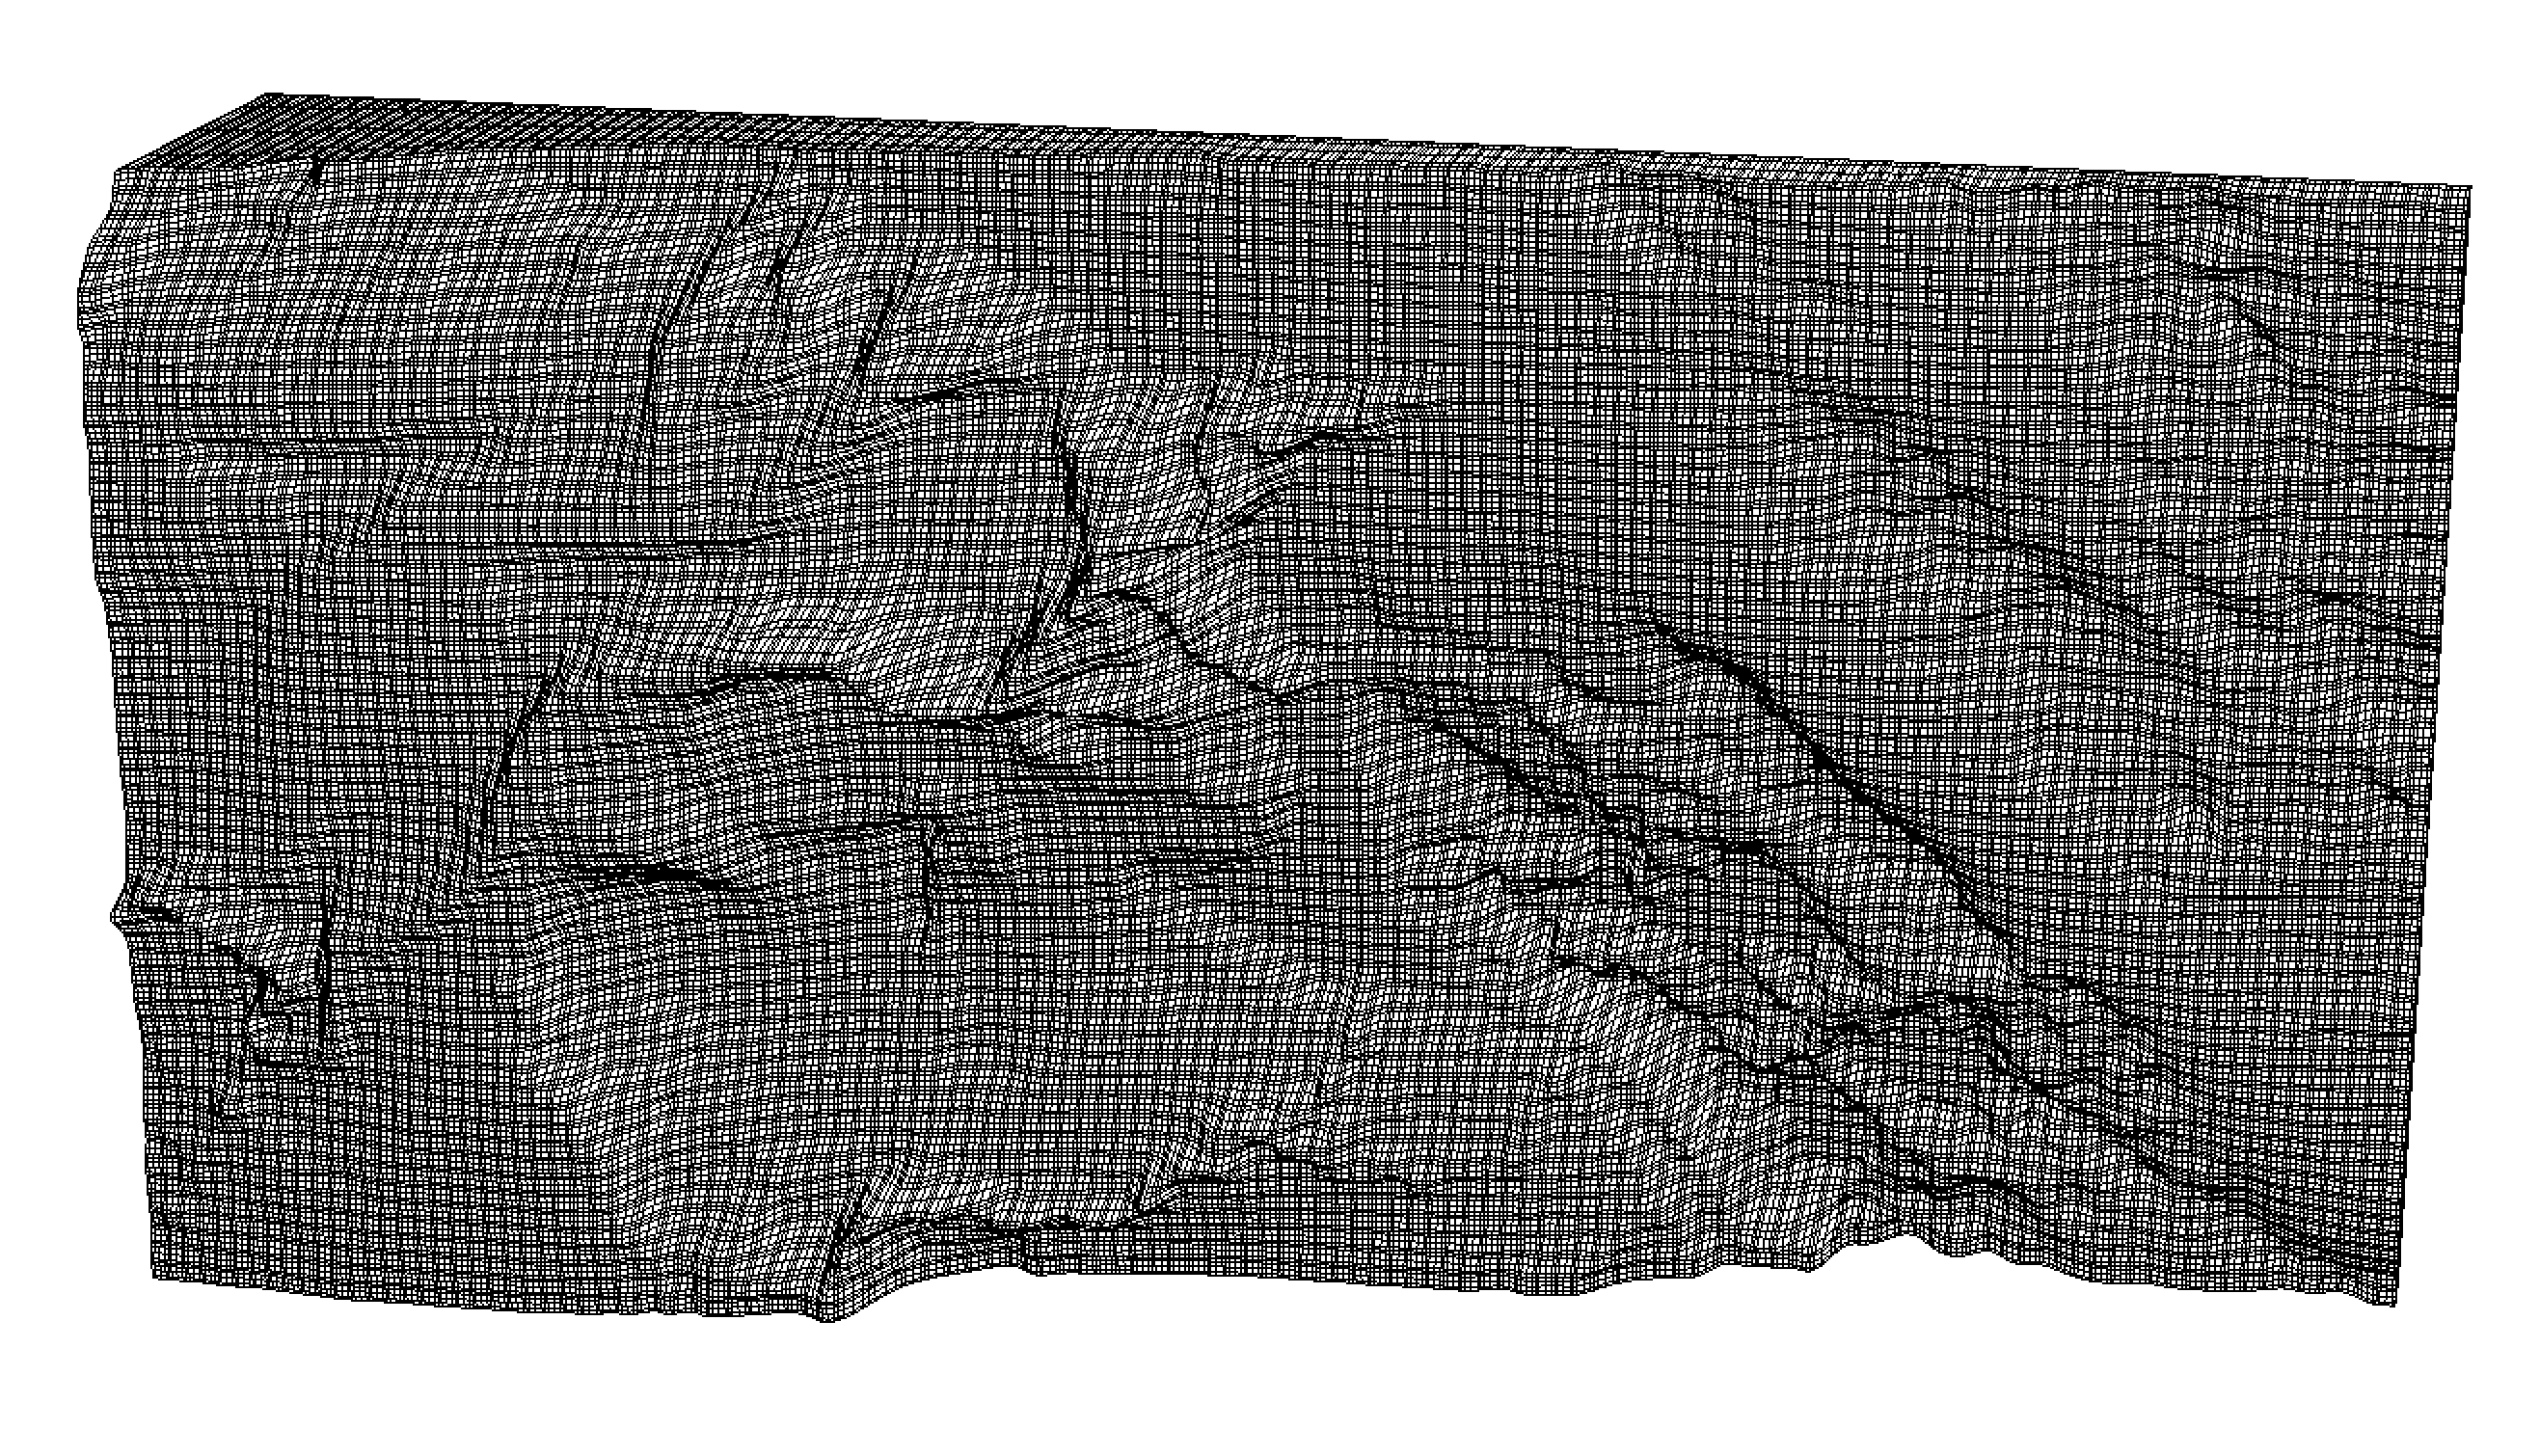
\includegraphics[width=\textwidth]{figures/monterey_with_grid.png}
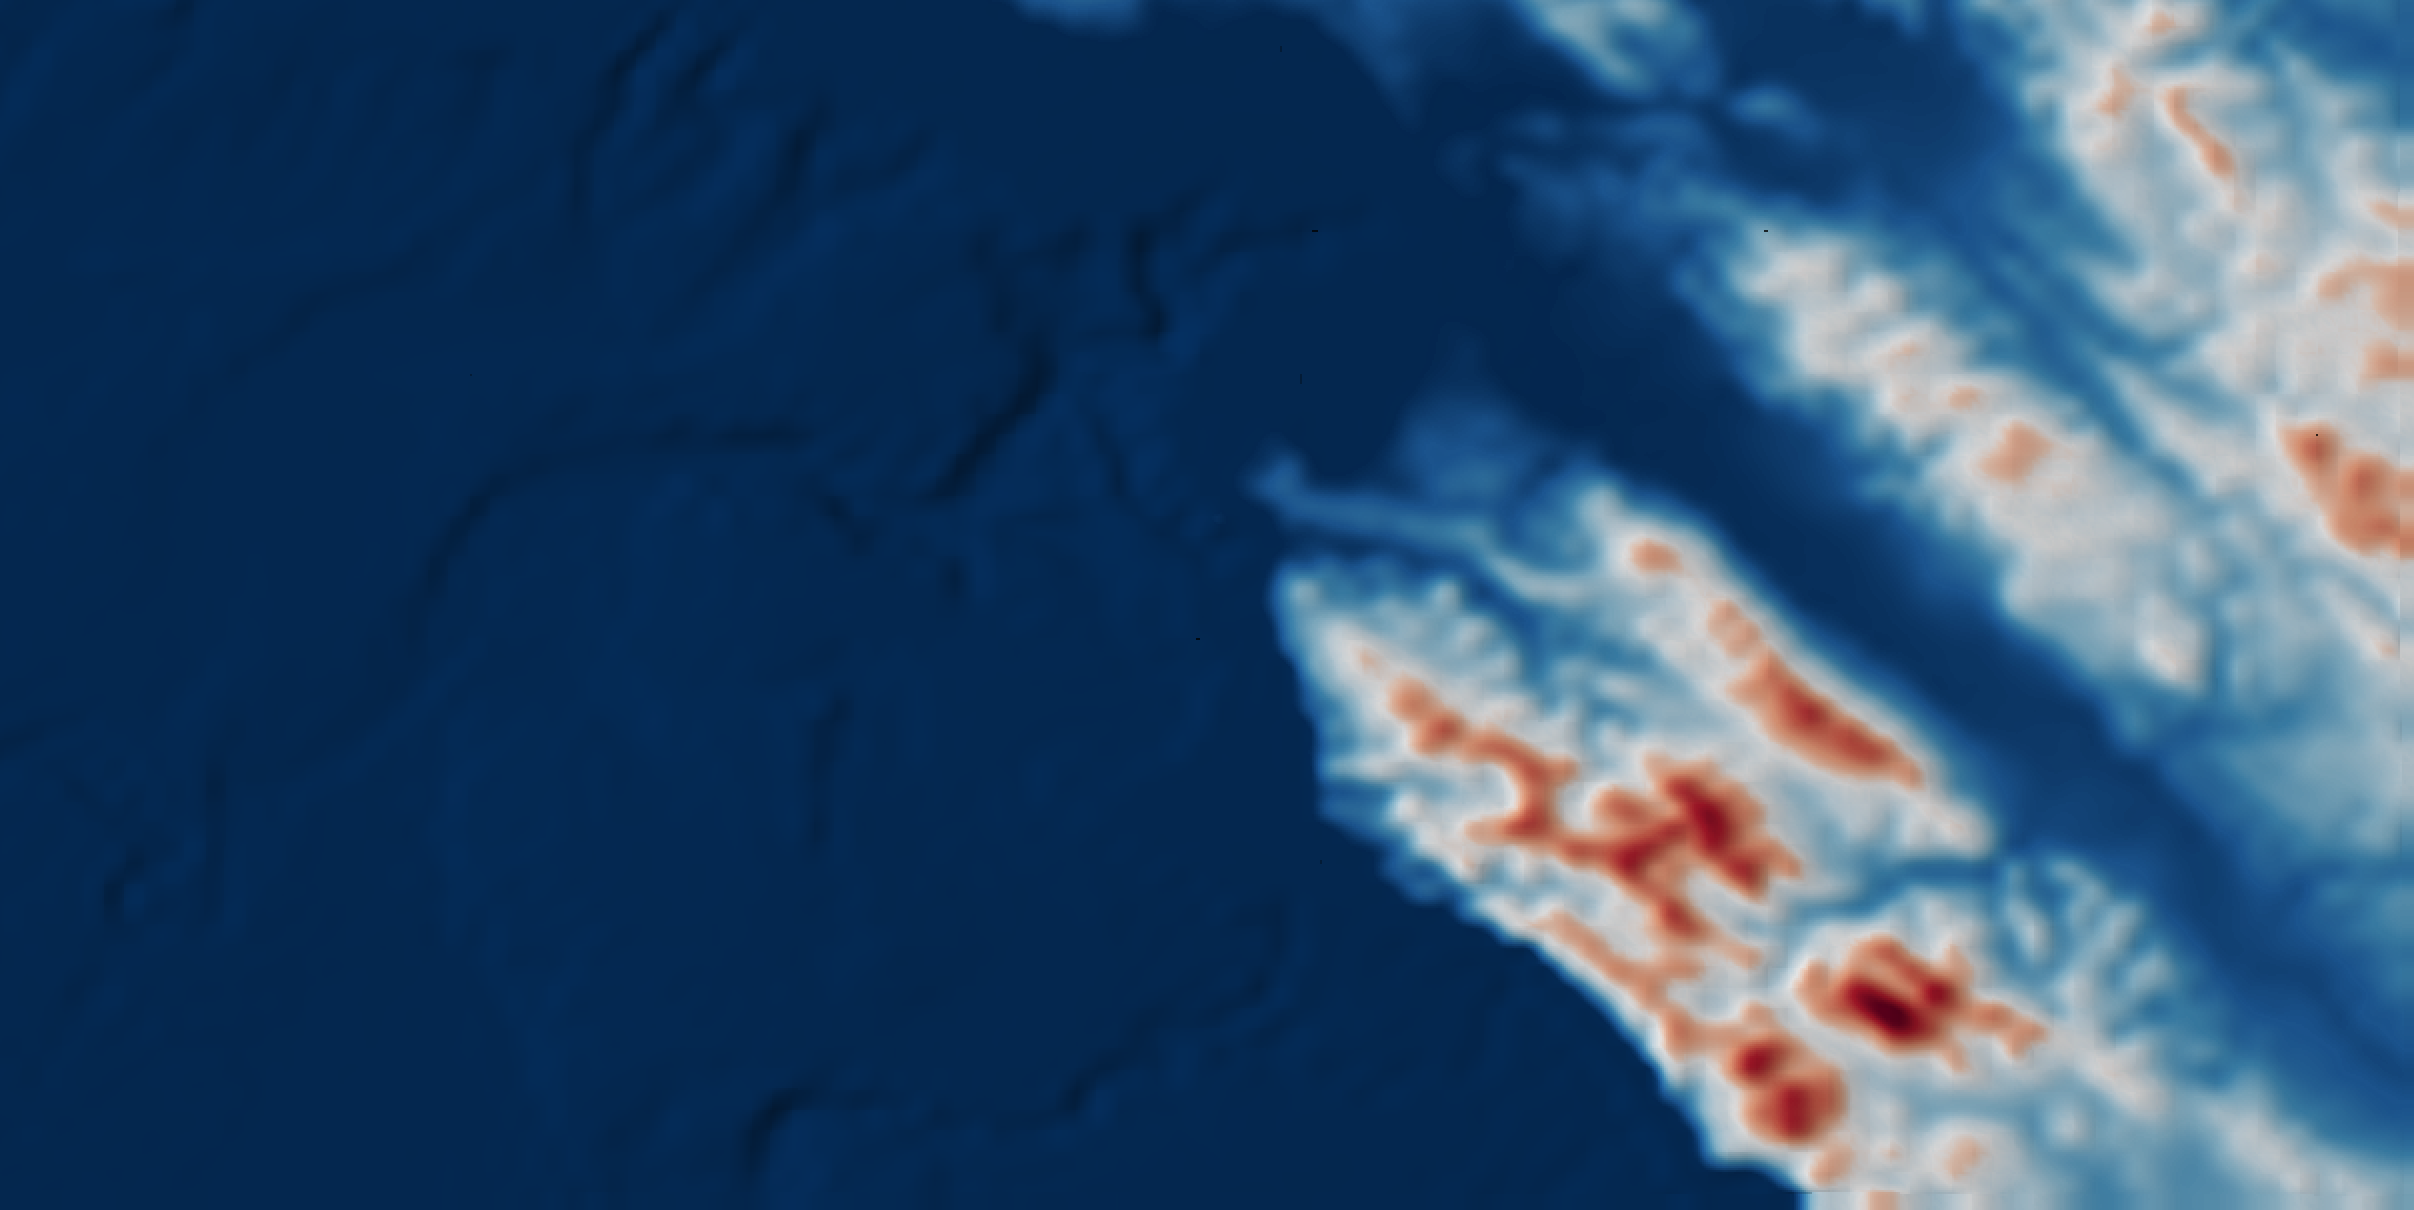
\includegraphics[width=\textwidth]{figures/monterey_colorscale.png}
\caption{Bottom view of the meshed Monterey Bay, California. The high order elements are visible in the top image whereas the topography is colored by its elevation in the bottom.}
\label{fig:montereySurfaceGrid}
\end{figure}

\begin{figure}[htbp]
\centering
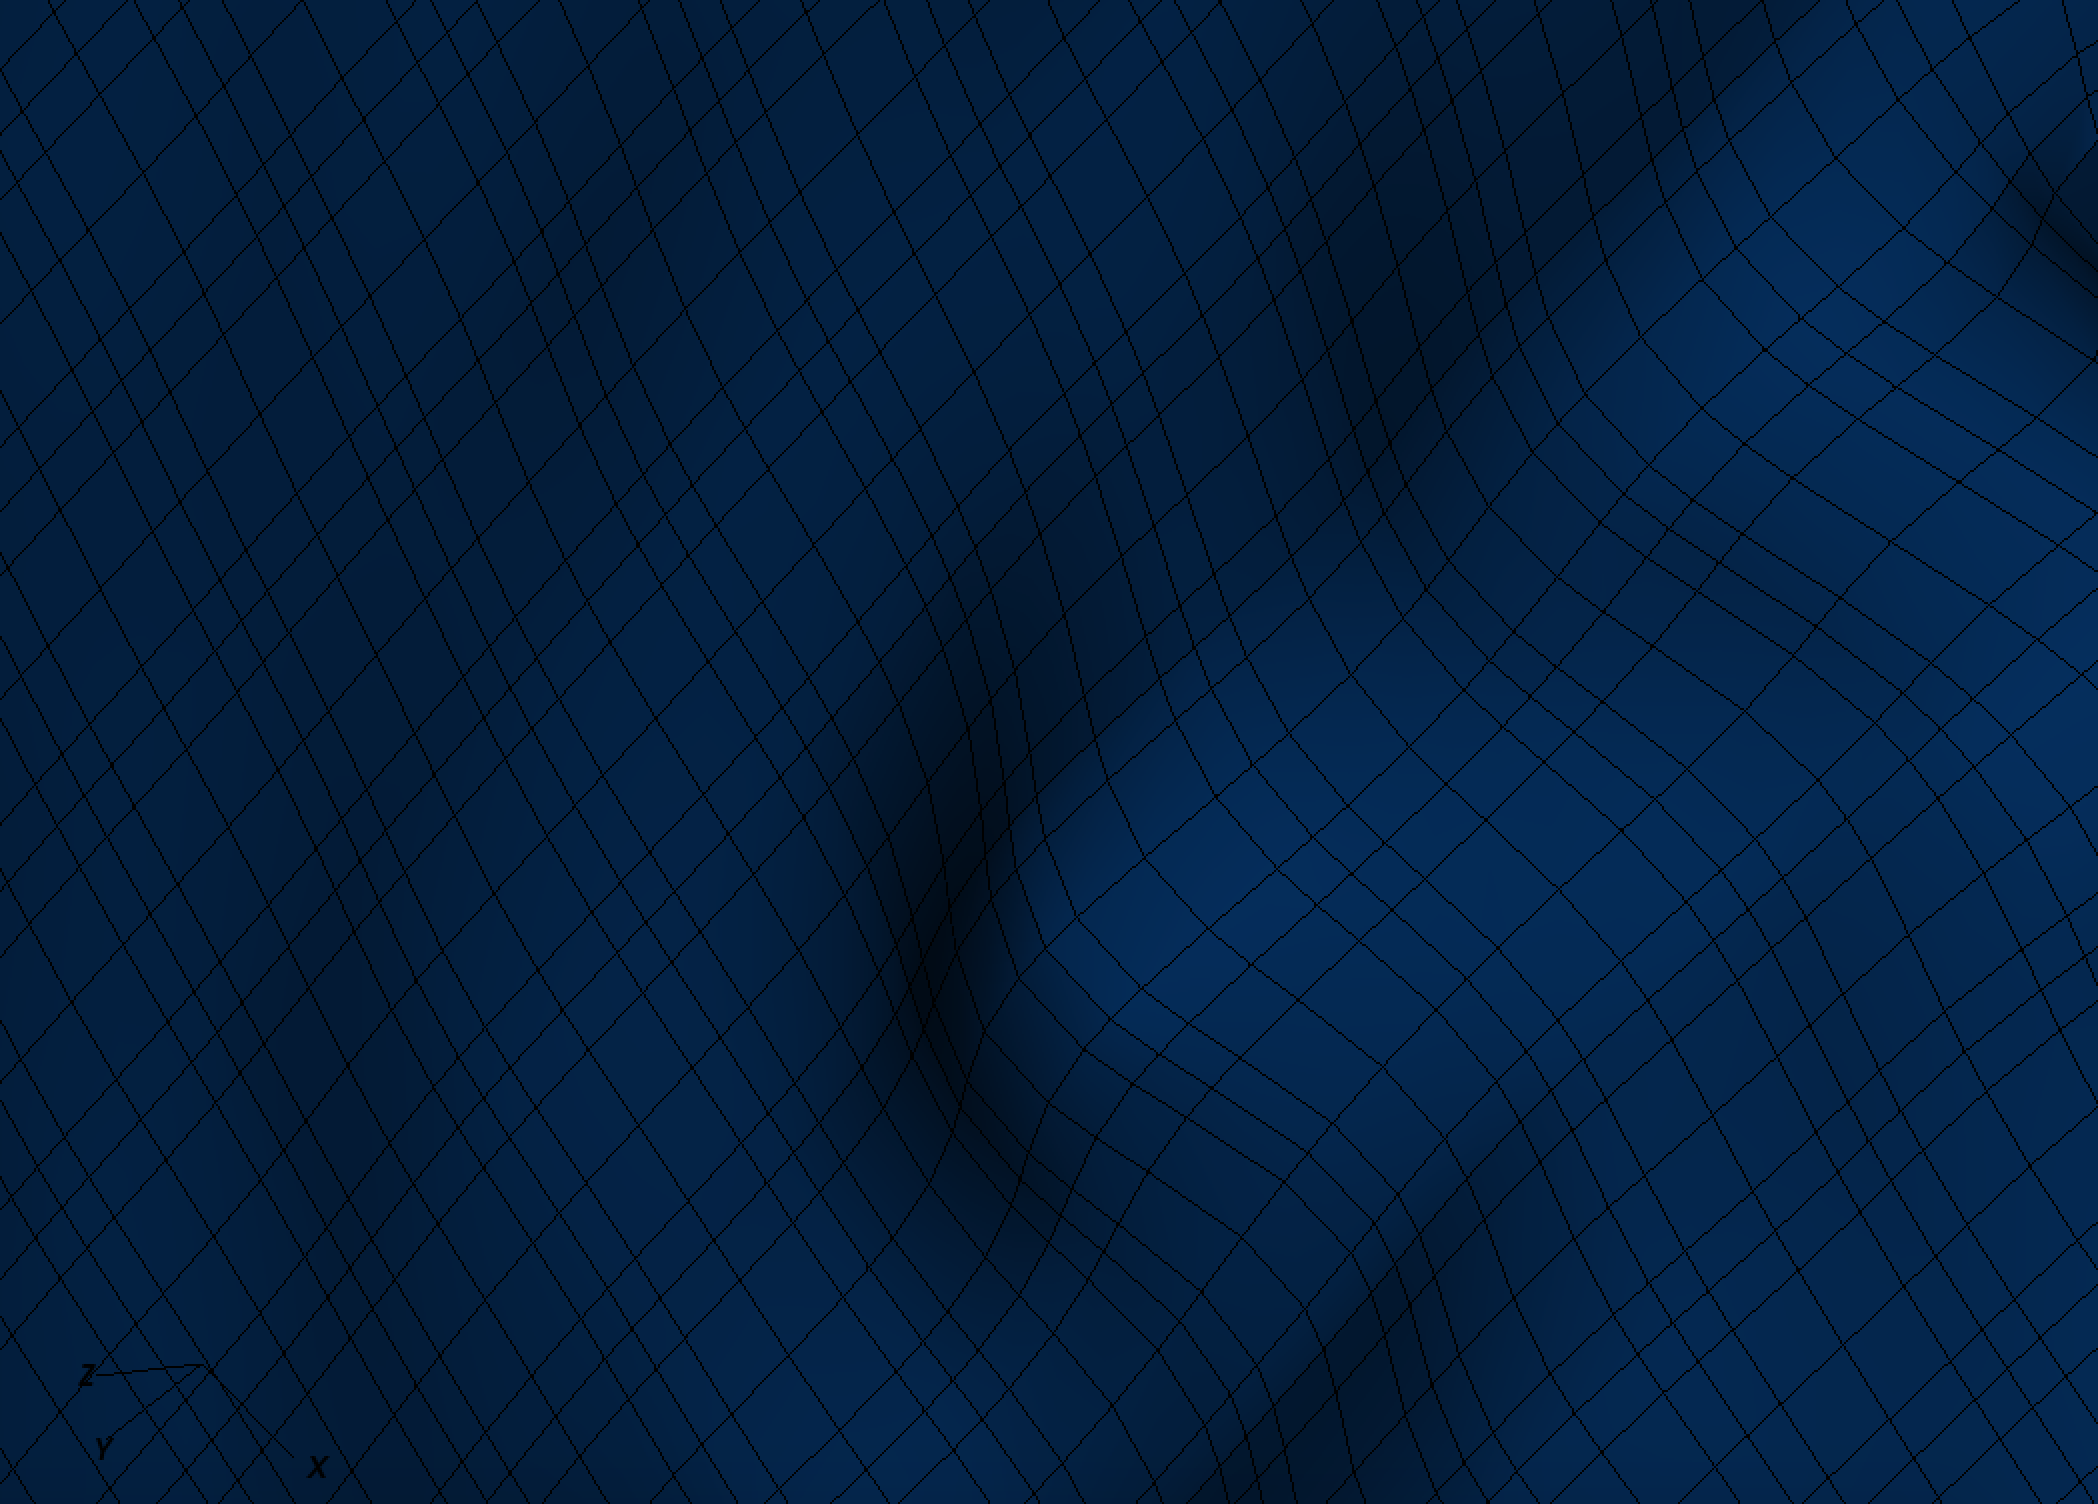
\includegraphics[width=\textwidth]{figures/GRID-detail.png}
\caption{A close view of the curved high order elements on the topography.}
\label{fig:gridDetailView}
\end{figure}

\subsection{Topography files and database}
The external topographic files are not incorporated into the CLIMA repository. 
They are automatically downloaded via a call to {\tt wget} from the {\tt Julia} driver into the user's working directory {\tt \$CLIMA\_HOME/USERS/TEST/DIRECTORY}. As of now, the available topography files are hosted here \url{https://web.njit.edu/~smarras/TopographyFiles} (notice: this directory is not directly accessible from the browser).

\hl{The grid reader should be enhanced to map the grid onto the sphere. As of now, the grid is read and mapped into a closed box only.}

\chapter{Benchmark Cases}

Here we describe a suite of test cases for dry and moist atmospheres, and for coarse-resolution global and higher-resolution limited-area model configurations. 

\hl{STILL INCOMPLETE}

\section{Held-Suarez (1994) Dry GCM Benchmark}

\citet{Held94} describe a simple and widely used setup for testing dry dynamical cores of GCMs. This setup is usually used to focus on statistically steady states (reached after about 100--400~days of spinup) but also lends itself to the study of the time-dependent evolution of Rossby waves and baroclinic instability. In this benchmark calculation, vertical SGS fluxes are usually set to zero; however, horizontal diffusion (or hyperdiffusion) is needed to damp the enstrophy cascade. 

\subsection{Initial Condition}

The initial condition for the Held-Suarez benchmark is an isothermal atmosphere at rest, with $T(t=0) = 300~\mathrm{K}$. Hydrostatically balanced initial density and pressure fields are calculated from the initial temperature according to section~\ref{s:initial_conditions}, and some small random perturbations are added to the density field to break the symmetry of the initial state and allow 3D baroclinic waves to develop. Baroclinic waves develop within a few simulated days in this benchmark calculation, and they begin to equilibrate after around 20--30~days. 

\subsection{Boundary Conditions}

The lower boundary condition is free-slip and thermally insulating, with no evaporation. That is, \emph{all} diffusive fluxes at the lower boundary (see section~\ref{s:bottom_bc}) are taken to be zero (if they are not already taken to be zero throughout the atmosphere, which is common in the Held-Suarez benchmark). With the vanishing surface fluxes, there is no need to specify a surface temperature.

\subsection{Sources}

\subsubsection{Momentum} 

Bottom drag in this benchmark calculation is modeled as a momentum sink in the lower part of the atmosphere, which is a function of velocity $\vec{u}$ and pressure $p$. The momentum sink takes the form of linear Rayleigh drag
\begin{equation}
    \vec{F}_u = -k_v(\sigma) \vec{u},
\end{equation}
where the drag coefficient decays away from the surface:
\begin{equation}
    k_v(\sigma) = k_f \max \left( 0, \frac{\sigma - \sigma_b}{1-\sigma_b} \right).
\end{equation}
Here,
\[
\sigma = \frac{p}{p_{\mathrm{MSLP}}}
\]
is a normalized pressure. (Usually, $\sigma$ is taken to be normalized by the temporally and spatially varying surface pressure $p_s$. But we can simplify this to a constant pressure.) \hl{[It would be good at some point to change this to the actual surface pressure, but this is not important now.]} The two parameters are
\begin{itemize}
    \item $\sigma_b = 0.7$: vertical extent of drag layer
    \item $k_f = 1~\mathrm{day^{-1}}$: drag coefficient at the surface
\end{itemize}.

\hl{Note that the momentum source appears in the momentum and energy equations. In hydrostatic models, the Rayleigh drag only acts on the horizontal velocity components and is zero in the vertical. Would that be easy to implement for us? Otherwise, also damping vertical velocities is ok for now, but it may need to strongly distorted upwelling and subsidence.}

\subsubsection{Heating/cooling}

Radiative heating/cooling is represented by linear relaxation of temperatures toward a radiative-equilibrium state with temperature \hl{[Note that here $p/p_{\mathrm{MSLP}}$ should be this, with a constant pressure for normalization. So generally, this is not equal to $\sigma$ above; it is only with the simplified $\sigma$ above.]}
\begin{multline}
    T_{\mathrm{eq}} = \max \\
    \left\{ T_{\mathrm{top}}, \left[ T_{\max} - (\Delta T)_y \sin^2 \phi - (\Delta \theta)_z \log\left(\frac{p}{p_{\mathrm{MSLP}}}\right) \cos^2 \phi \right]
    \left( \frac{p}{p_{\mathrm{MSLP}}} \right)^{\kappa} \right\}.
\end{multline}
Here, $\phi$ is latitude, $\kappa = R_d/c_{pd}$ is the adiabatic exponent, and the default values of the parameters are:
\begin{itemize}
    \item $T_{\mathrm{top}} = 200~\mathrm{K}$: temperature at model top
    \item $T_{\max} = 315~\mathrm{K}$: near-surface temperature at equator
    \item $(\Delta T)_y = 60~\mathrm{K}$: pole-equator temperature difference in radiative equilibrium
    \item $(\Delta \theta)_z = 10~\mathrm{K}$: static stability in background state.
\end{itemize}

Relaxation of temperatures toward the background state on a timescale $k_T^{-1}$ implies a source in the energy equation that is a function of latitude $\phi$, pressure $p$, and temperature $T$:
\begin{equation}
    Q =  - c_{vd} k_T(\phi, p) (T - T_{\mathrm{eq}}).
\end{equation} 
The relaxation coefficient $k_T$ is taken to vary with latitude and normalized pressure $\sigma$ as
\begin{equation}
k_T(\phi, p) = k_a + (k_s - k_a) \max\left(0, \frac{\sigma - \sigma_b}{1-\sigma_b}\right) \cos^4 \phi ,
\end{equation}
where 
\begin{itemize}
    \item $k_a = (40~\mathrm{day})^{-1}$: relaxation coefficient in interior atmosphere
    \item $k_s = (4~\mathrm{day})^{-1}$: relaxation coefficient  at equator near the surface.
\end{itemize}
The interior relaxation timescale $k_a^{-1}$ controls the timescale over which they flow equilibrates to a statistically steady state

\subsection{SGS Fluxes}

In global models with a stratified atmosphere, large-scale turbulence with Rossby waves usually dominates the kinetic energy of the flow. The large-scale flow is primarily rotational and horizontal. SGS dissipation primarily needs to absorb the cascade of enstrophy (vorticity variance) to small scales. This is usually accomplished by horizontal hyperdiffusion.

Hence, the SGS mixing needs to be strongly anisotropic, e.g., as outlined in section~\ref{s:anisotropic_SGS_mixing}.

\section{2D Rising Thermal Bubble (Robert 1993)}
\label{2dRTBtest}
This test is described \cite{robert1993}. It consists of a flow that is triggered by the thermal perturbation of a neutrally stratified atmosphere at initially uniform potential temperature $\theta_0 = 303$ K
and in hydrostatic equilibrium such that the pressure decreases with $z$ as:
\begin{equation}
\label{pressureDistrib}
p = p_{0}\left(1-\frac{g}{c_p{\theta_{0}}}z\right)^{c_p/R}.
\end{equation}
The domain $\Omega=[-5000,5000]\times[0,10000]\,\mathrm{m}^2$.
The perturbation is linear and defined as
\begin{equation}
 \Delta\theta = \left\{ \begin{array}{ll}
 \theta_c & \mathrm{if } r \leq a=50\,{\mathrm K}\\
 \theta_c e^{-(x - a)^2/\sigma^2} & \mathrm{if } r > a=50\,{\mathrm K}\\
\end{array} \right.
\label{eq:robertIni}
\end{equation}
where $r = \sqrt[]{(x-x_{c})^{2} + (z-z_{c})^{2}}$, $(x_c,z_c) = (500,260)\,\mathrm{m}$, $\sigma = 100$, and $\theta_c=0.5$ K.

\begin{figure}[htbp]
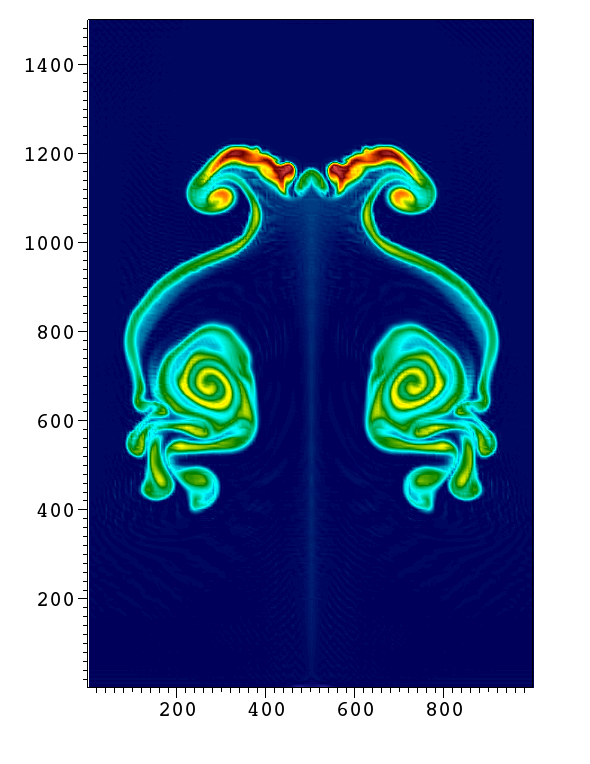
\includegraphics[width=\textwidth]{figures/RTB-Robert--smgo-5mX5m-1080s0000.png}
\caption{2D rising thermal bubble (Robert, 1993) stabilized via a constant coefficient Smagorinsky-Lilly SGS: Potential temperature, $\theta$, at $t=1080\,\mathrm{s}$. Grid resolution: $\Delta x = \Delta z = 5\,\mathrm{m}$.}
\label{fig:benchmarks/robert5msmago}
\end{figure}

\section{2D Density Current}
This test is described in \cite{strakaWilhelmson1993}. It consists of a flow that is triggered by the cold perturbation of a neutrally stratified atmosphere at initially uniform potential temperature $\theta_0 = 300$ K
and in hydrostatic equilibrium such that the pressure decreases with $z$ as:
\begin{equation}
\label{pressureDistrib2}
p = p_{0}\left(1-\frac{g}{c_p{\theta_{0}}}z\right)^{c_p/R}.
\end{equation}
The domain $\Omega=[-25600,25600]\times[0,6400]\,\mathrm{m}^2$.
The perturbation is linear and defined as
\begin{equation}
 \Delta\theta = \left\{ \begin{array}{ll}
 0 & \mathrm{if } r > 1\,{\mathrm K}\\
 0.5 \theta_c \left(1 + \cos(\pi r) \right) \leq 1\,{\mathrm K}\\
\end{array} \right.
\label{eq:robertIni2}
\end{equation}
where $r = \sqrt[]{(x-x_{c})^2/r_x^{2} + (z-z_{c})^{2}/r_z^2}$, $(x_c,z_c) = (0,4000)\,\mathrm{m}$, $(r_x, r_z) = (4000, 2000)\,\mathrm{m}$ and $\theta_c=-15$ K. The fully developed density current at $t=900\,\mathrm{s}$ simulated with a grid effective resolution of $25$ m in both spatial directions is shown in Figure \ref{fig:benchmarks/dc25msmago}.

\begin{figure}[htbp]
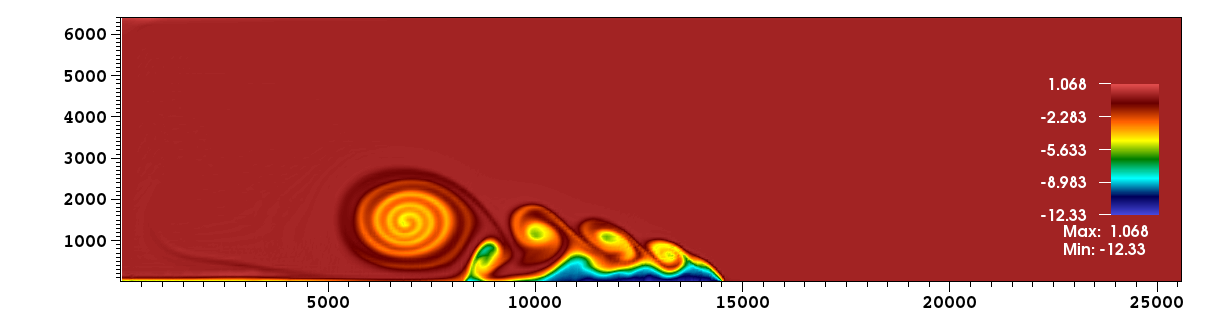
\includegraphics[width=1.2\textwidth]{figures/DC-smgo-25mx25m-900s0000.png}
\caption{2D density current stabilized via a constant coefficient Smagorinsky-Lilly SGS. Potential temperature, $\theta$, at $t=900\,\mathrm{s}$ (top) and at $t=1200\,\mathrm{s}$ (bottom). Grid resolution: $\Delta x = \Delta z = 25\,\mathrm{m}$.
}
\label{fig:benchmarks/dc25msmago}
\end{figure}


%%
\section{Rising Thermal Bubble in a Saturated Atmosphere}
\label{rtb3D}
The moist dynamics is tested by means of the saturated rising bubble test described in \cite{Pressel15a}. The initial conditions are setup as follows:

\begin{itemize}
\item Initialize dry atmosphere with uniform background $\theta_{ref} = 320$ K
\item Add thermal perturbation $\Delta \theta$ of radius $r=2$ km
\item Set a uniform total mixing ratio $q_t = 0.0192 \,\mathrm{kg/kg}$ and $q_l = q_i = 0.0\,\mathrm{kg/kg}$
\item Calculate the gas constants for moist air: 
\[\begin{array}{lcl}
R_{gas} &=& {\tt MoistThermodynamics.gas\_constant\_air(q_t, q_l, q_i)}\\
c_v     &=& {\tt MoistThermodynamics.cv\_m(q_t, q_l, q_i)}\\
c_p     &=& {\tt MoistThermodynamics.cp\_m(q_t, q_l, q_i)}\\
\end{array}
\]
\item  Compute $\theta$, $\rho$, and $T$ as if the background were dry:\\
    \[ \begin{array}{lcl}
  \theta &=& \theta_{ref} + \Delta\theta\\
 \pi & =& 1 - gz/(c_p\theta)\\
 \rho & = & p_0/(R_{gas}\theta)\pi^{c_v/R_{gas}}\\
 T   & = &\pi \theta
\end{array}\]

\item Add the contribution of moisture to the internal energy and recalculate $T$ and $P$, and obtain $e^{\rm tot}$ using the following {\tt MoistThermodynamics} functions:
\[\begin{array}{lcl}
I &=& {\tt MoistThermodynamics.internal\_energy(T + T_0, q_t, q_l, q_i)}\\
T &=& {\tt MoistThermodynamics.air\_temperature(I, q_t, q_l, q_i)}\\
P &=& {\tt MoistThermodynamics.air\_pressure(T - T_{ref} , \rho, q_t, q_l, q_i)}\\
e^{\rm tot} &=& {\tt MoistThermodynamics.total\_energy(0.5\|{\bf u} \|^2, gz, T, q_t)}
\end{array}\]
\end{itemize}

%%
\section{Dynamics and Chemistry of Marine Stratocumulus: DYCOMS RF01}

\subsection{Initial Condition}

\cite{Stevens05a} provide the following initial distributions of liquid water potential temperature,
\begin{equation}\label{eq:dycoms1}
\theta_l(z) = 
    \begin{cases}
    289.0\;\mathrm{K} & z\leq z_i,\\
    297.5 + (z - z_i)^{1/3}\;\mathrm{K}& z > z_i,
    \end{cases}
\end{equation}
and total specific humidity, 
\begin{equation}\label{eq:dycoms2}
q_t(z) = 
    \begin{cases}
    q_{t,0} & z\leq z_i,\\
    1.5\;\mathrm{g/kg} & z > z_i.
    \end{cases}
\end{equation}
Here, $z_i$ is the initial cloud top set to $z_i=840\,\mathrm{m}$. \cite{Stevens05a} state that ``modeling groups were also asked to standardize their thermodynamic calculations'' so that the initial state corresponds to a cloud layer between 600 and 800~m with liquid water specific humidity
\begin{equation}\label{eq:dycoms3}
q_l(z) = 
    \begin{cases}
    0 & z\leq 600~\mathrm{m},\\
    0.45\frac{{}z - 600~\mathrm{m}}{z_i - 600~\mathrm{m}}\;\mathrm{\frac{g}{kg}}   & 600~\mathrm{m} < z \leq z_i,\\
    0 & z > z_i.\\
    \end{cases}
\end{equation}
With our thermodynamics and standard thermodynamical constants, we obtain such a cloud layer if we choose the initial total specific humidity in the mixed layer to be $q_{t,0} = 8.1\;\mathrm{g/kg}$, which is slightly lower than the DYCOMS default value of $9\;\mathrm{g/kg}$. (An alternative to modifying the initial $q_{t,0}$ would be to adjust, e.g., the latent heat of vaporization or the vapor pressure at the triple point to obtain the desired cloud layer with $q_{t,0} = 9\;\mathrm{g/kg}$.)

To specify the thermodynamic state completely, we additionally need to specify an initial density. We do so by first specifying an initial pressure
\[
p_0(z) = p_{s} \exp(-z/H), \qquad H = \frac{R_m T_{BL}}{g},
\]
where $R_m = R_m(q_t, q_l)$ is the gas constant for moist air, $T_{BL} = 285.0~\mathrm{K}$ is an average boundary-layer temperature, and $p_s = 1.0178\times 10^{5}~\mathrm{Pa}$ is the surface pressure, with surface density $\rho_s = 1.22~\mathrm{kg/m^3}$ and surface temperature $T_s = p_s/(\rho_s R_{m,s})$. Consistent with the Boussinesq or anelastic approximation used in most DYCOMS simulations, we calculate thermodynamic quantities with this reference pressure $p_0(z)$. We use the linearized expression for the liquid-water potential temperature,
\begin{equation}
    \label{eq:betts1973}
    \theta_l = \theta \left(1 - \frac{L_{v,0} q_l}{c_{pm} T} \right) = \theta - \frac{L_{v,0} q_l}{c_{pm} \Pi_0},
\end{equation}
where $\theta = T/\Pi_0$, and 
\[
\Pi_0 = \left( \frac{p_0(z)}{p_{s}} \right)^{R_d/c_{pd}}
\]
is evaluated with the pressure profile $p_0(z)$. This can be solved for temperature as a function of height $z$,
\[
T = \Pi_0 \theta_l + \frac{L_{v,0} q_l}{c_{pm} \Pi_0},
\]
given $\theta_l(z)$, $q_l(z)$, and $\Pi(z)$. Density is then obtained from the ideal gas law as
\[
\rho(z) \approx \frac{p_0(z)}{R_m T(z)},
\]
thus completely specifying the initial state. 

The initial state of all the quantities described above are plotted in Figure \ref{dycomsInitFig}
\begin{figure}
    \centering
	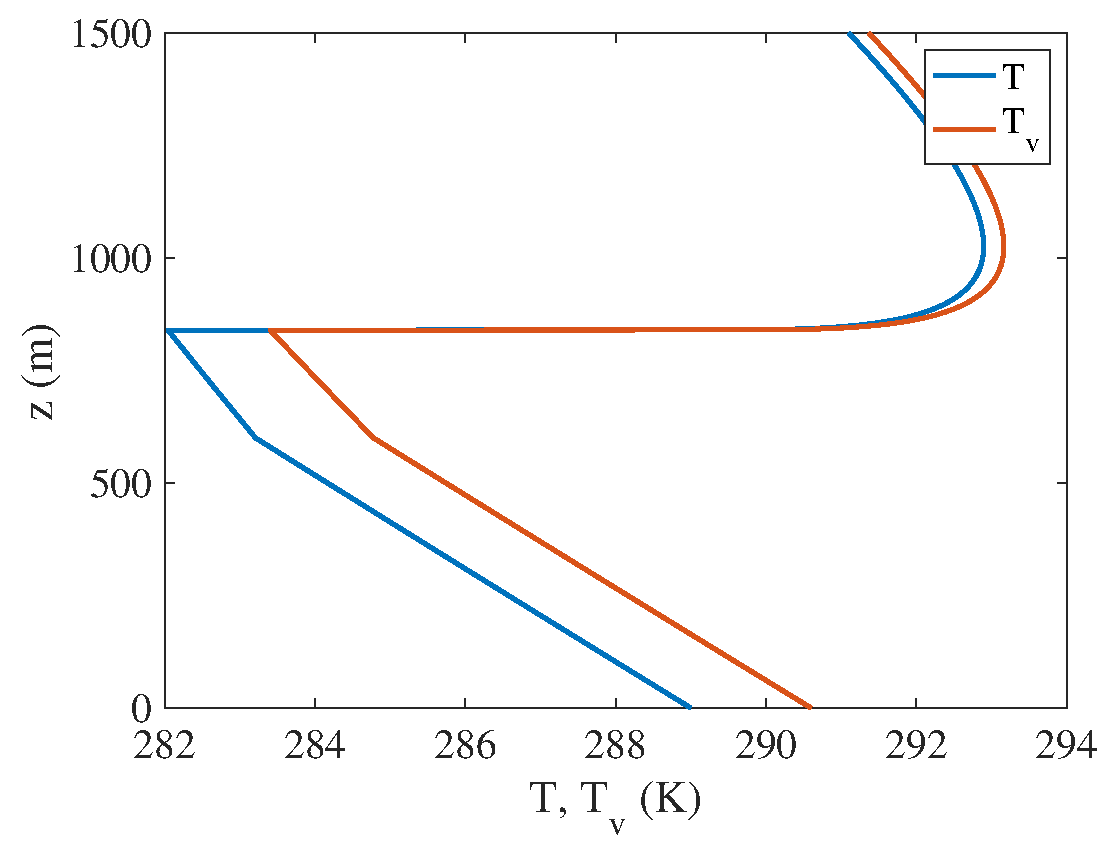
\includegraphics[width=0.49\textwidth]{./figures/dy_tempe.eps}
	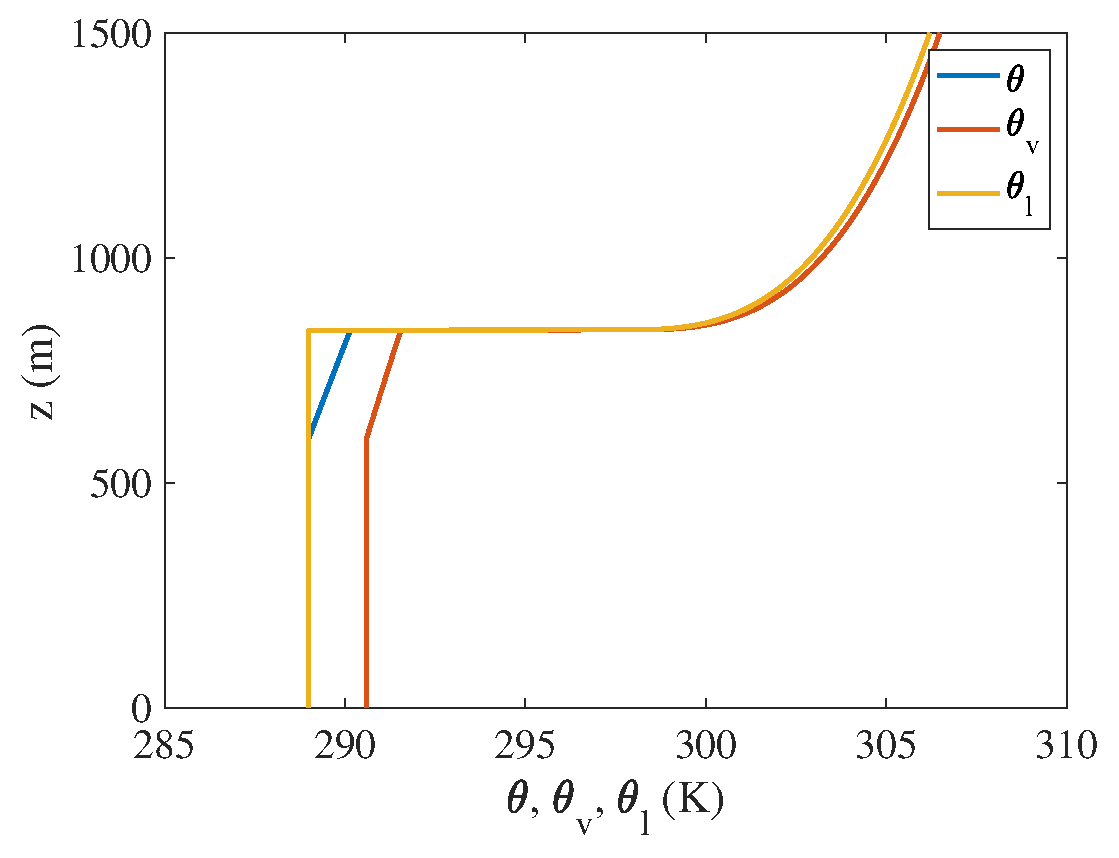
\includegraphics[width=0.49\textwidth]{./figures/dy_pot_temp.eps}
	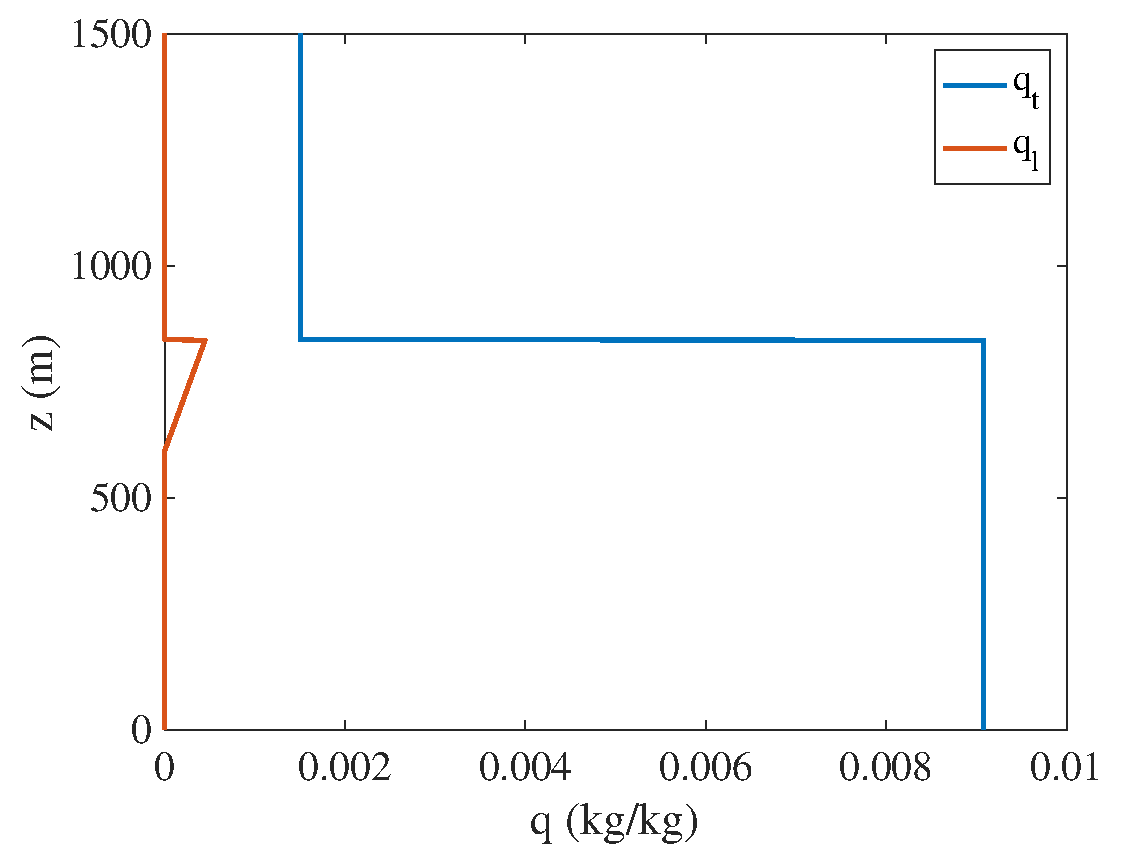
\includegraphics[width=0.49\textwidth]{./figures/dy_mixing_ratios.eps}
	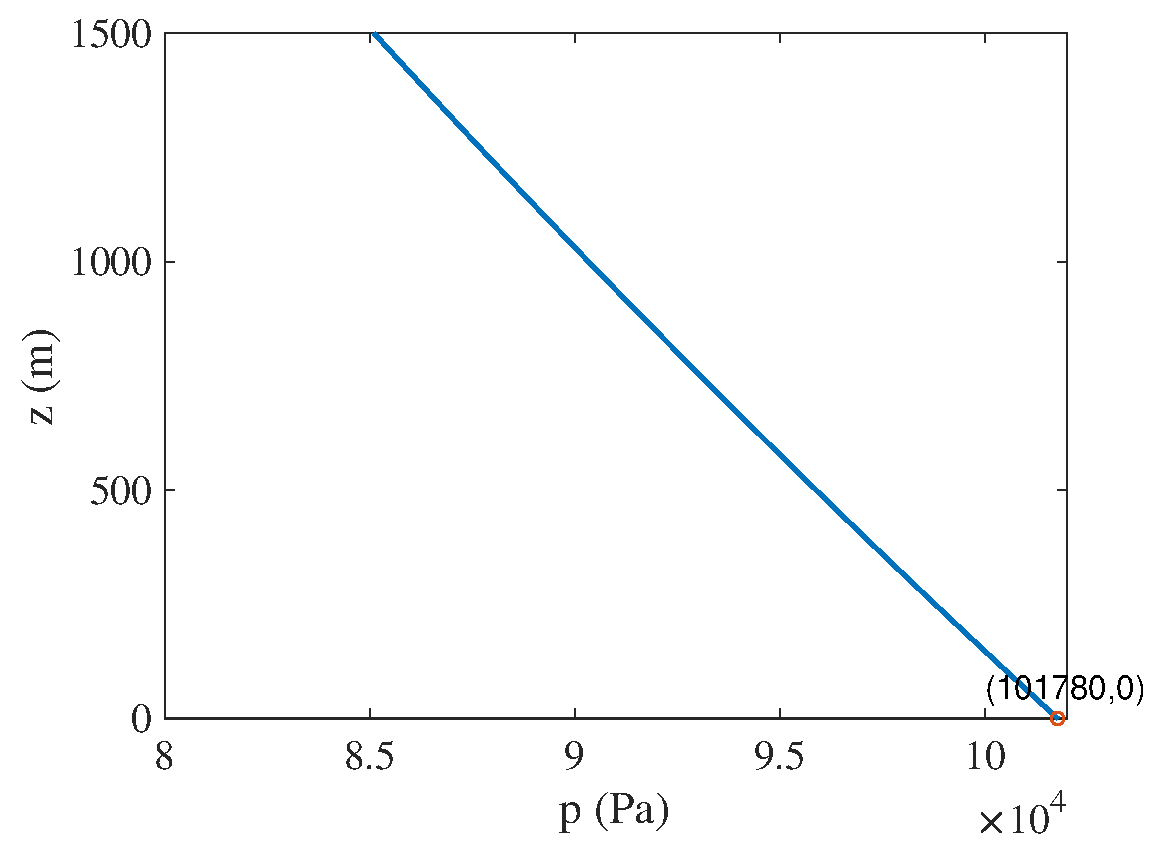
\includegraphics[width=0.49\textwidth]{./figures/dy_press.eps}
	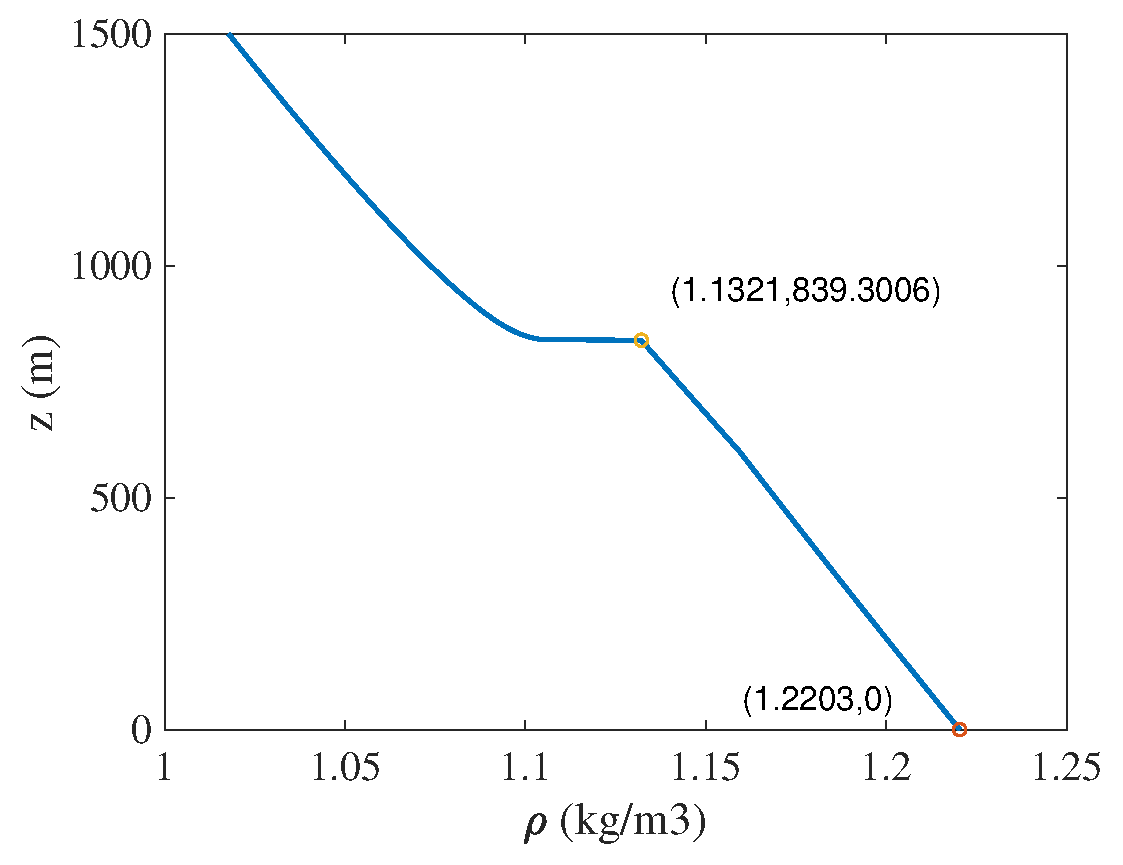
\includegraphics[width=0.49\textwidth]{./figures/dy_densi.eps}
	%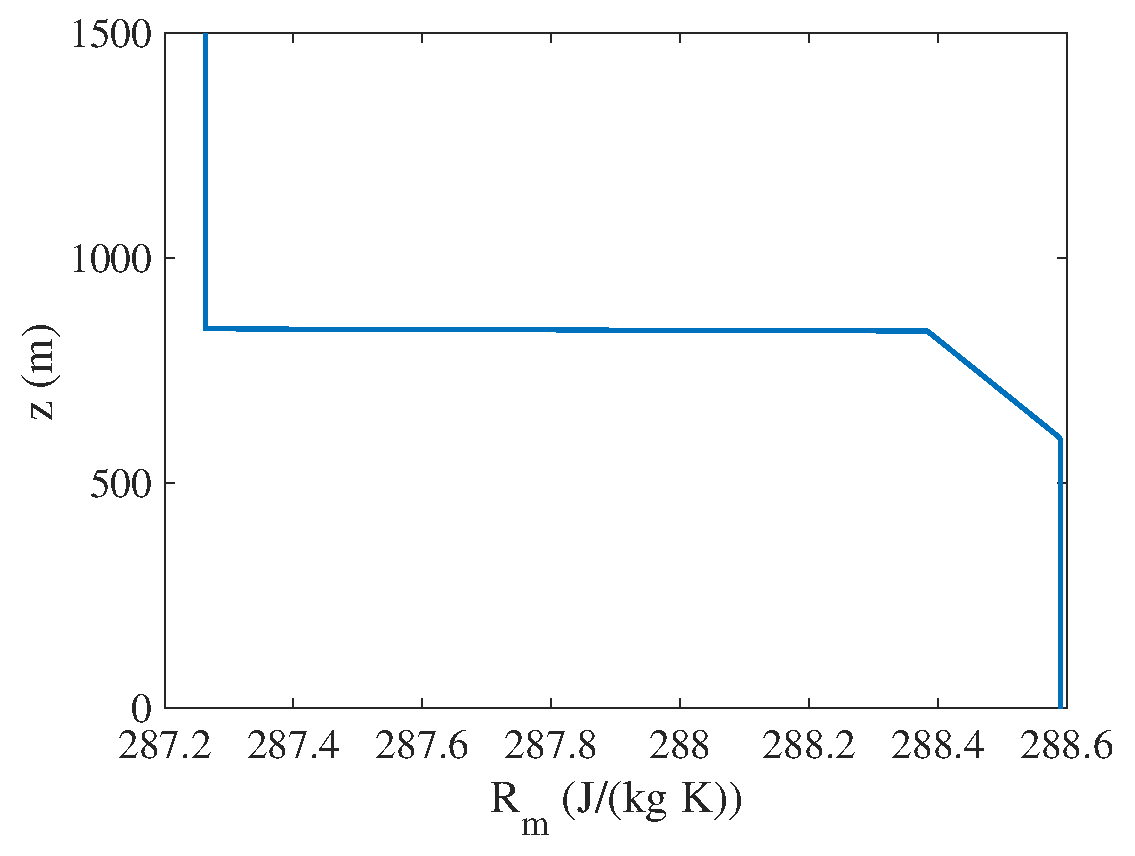
\includegraphics[width=0.49\textwidth]{./figures/dy_Rm.eps}
	%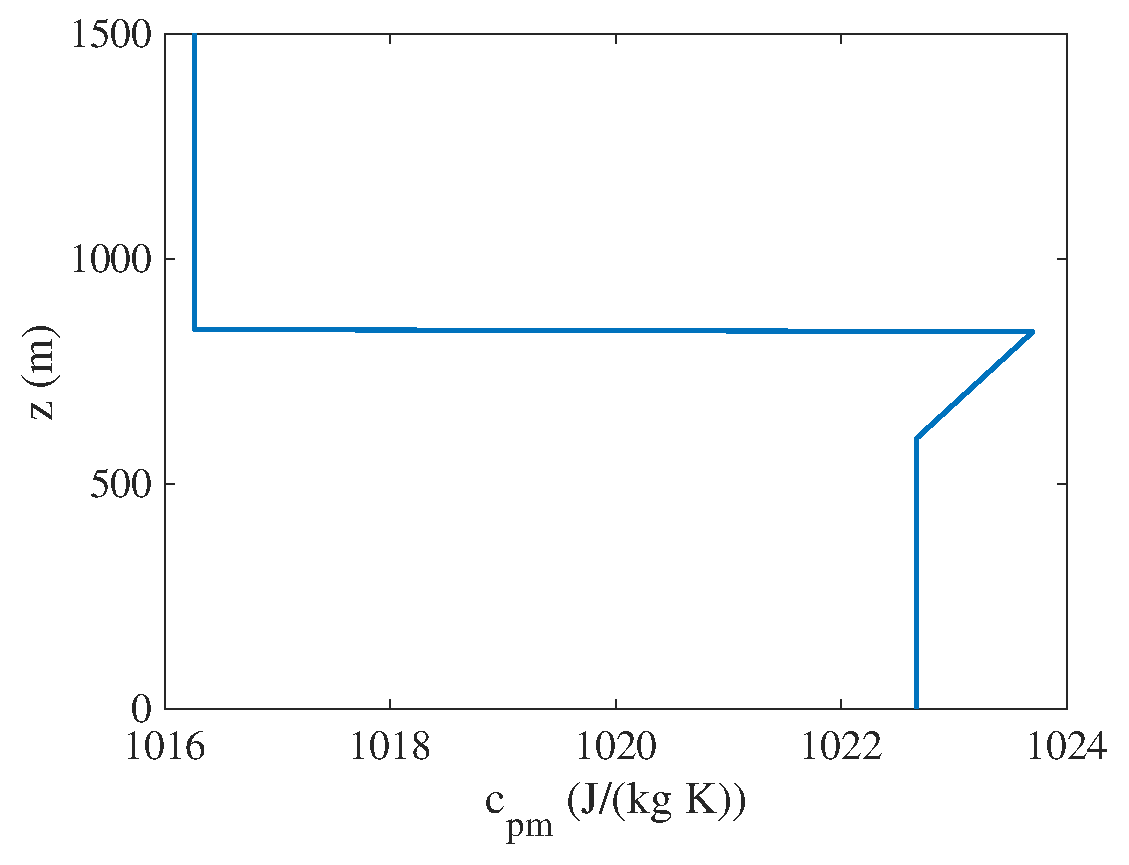
\includegraphics[width=0.49\textwidth]{./figures/dy_cpm.eps}
      \caption{Dycoms: initial states of $T, T_v, \theta, \theta_v, \theta_l, q_t, q_l, p, \rho$.}
\label{dycomsInitFig}
\end{figure}

\subsection{Boundary Conditions}

The bottom boundary conditions for DYCOMS are prescribed energy and water fluxes and a drag law for momentum, as described in section~\ref{s:bottom_bc}. The prescribed fluxes at the surfaces are
\begin{itemize} 
\item Sensible heat flux $\mathrm{SHF} = \vec{n} \cdot (\rho \vec{J}_{\mathrm{sfc}}) = 15\,\mathrm{W/m^2}$
\item Latent heat flux $\mathrm{LHF} = \vec{n} \cdot (\rho \vec{D}_{\mathrm{sfc}}) = 115\,\mathrm{W/m^2}$
\item Energy flux $\vec{n} \cdot \rho (\vec{J}_{\mathrm{sfc}} + \vec{D}_{\mathrm{sfc}}) = \mathrm{LHF + SHF} = 130\,\mathrm{W/m^2}$
\item Evaporation $E \approx \mathrm{LHF}/L_{v,0}$
\end{itemize}

\subsection{Sources}

\subsubsection{Radiative cooling}
Radiative cooling is imposed through the simple model described by \cite{Stevens05a}. It specifies the vertical radiative energy flux $\Frad = F_R \vec{k}$ (part of the non-diffusive energy fluxes \eqref{eq:ndf_flux}) as
\begin{equation}
    \label{e:radiativeStevens05}
    F_{R}({\bf x}, t) = F_0{\rm e}^{-Q(z,\infty)} +
    F_1{\rm e}^{-Q(0, z)} +
    \rho_i c_{pd} D \alpha_z\frac{(z-z_i)^{4/3}}{4} + z_i(z - z_i)^{1/3}
\end{equation}
where 
\begin{equation}
    Q(a,b) = \kappa\int_{a}^{b}\rho\,q_l\,dz.
\end{equation}
The following parameters are used:
$F_0=70\,\mathrm{W\,m^{-2}}$, $F_1=22\,\mathrm{W\,m^{-2}}$, $\kappa=85\,\mathrm{m^2\,kg^{-1}}$, $\alpha_z=1\,\mathrm{m^{-4/3}}$. The parameter $D=3.75\times 10^{-6}\,\mathrm{s^{-1}}$ gives the large-scale divergence, which also enters the dynamical equations as an additional advection term.  

\subsubsection{Large-scale subsidence}

A large-scale subsidence velocity $W=-Dz$ is imposed and is added to the internally generated vertical velocity $w$ in all governing equations. 

\subsection{SGS Fluxes}

The interaction of the resolved flow with SGS fluxes is crucial for a successful simulation of stratocumulus \citep{Pressel17a}. If there is too much spurious mixing across the sharp inversion interface, the clouds dissipate because too much dry air from above the clouds is mixed into the clouds. Hence, it is important to use SGS schemes that limit mixing near the stable inversion interface.

\section{3D Squall Line}
\label{sq3D}
The three-dimensional simulation of a squall line is defined in the domain 
$80\times 80\times20\,\mathrm{km}^3$. 
The initial background state is given by the sounding of \cite{gabersekGiraldoDoyle2012}.
To initiate the vertical transport of water vapor to a level of condensation (and hence trigger a cloud formation, the initial background is forced by a temperature anomaly $\theta'$ $3$ K warmer than the surrounding environment. 

A stretched grid along $z$ is used to make the resolution higher in the lower atmosphere where convection is triggered.
The domain is crossed by a horizontal wind along the x-direction with a $12\,\mathrm{m\,s^{-1}}$ shear at $z=2000\,\mathrm{m}$.
A no-slip condition is applied on the surface boundary while periodic boundaries are defined along $x$ and $y$. 
To damp the vertically propagating gravity ways triggered by the cloud formation, a Rayleigh absorbing layer is applied at the higher layers of the atmosphere.
The cloud first forms at approximately 500 s, and is fully develop after 4500 s. 
An instantaneous view of the precipitating squall line is shown in Figure \ref{fig:benchmarks/squall1}. 

\begin{figure}[htbp]
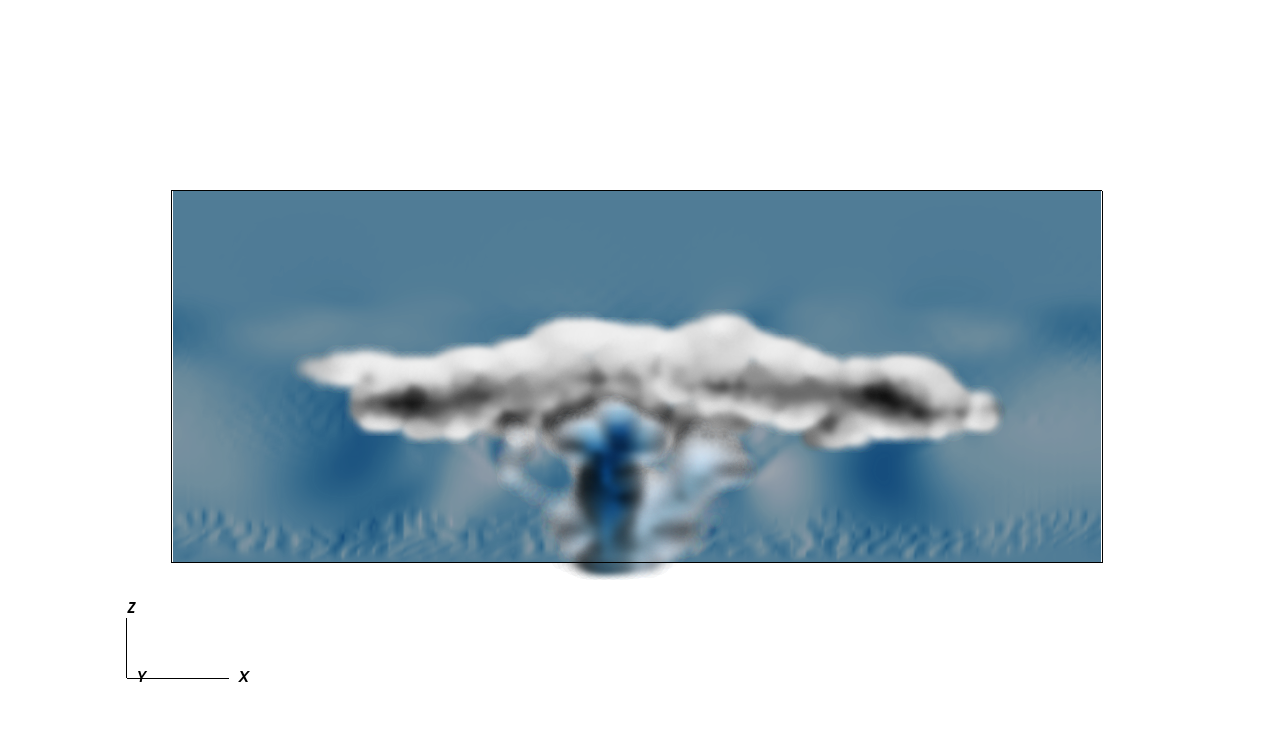
\includegraphics[width=1.2\textwidth]{figures/squall_working_warm_rain_frontal_view0028.png}
\caption{Front view of a fully developed squall line with precipitating rain. }
\label{fig:benchmarks/squall1}
\end{figure}


\section{External Soundings}
External soundings can be read into the code for initialization purposes. The sounding requires the format reported in Table \ref{tab:DeltaDefinitionsTable}.

\begin{table*}[t]
\centering
{\footnotesize
\caption[short]{Structure of sounding files for simulation initialization.}
\label{tab:DeltaDefinitionsTable}
\begin{tabular*}{\textwidth}{ @{\extracolsep{\fill}} llllll}
\hline
\hline
z (m) & $\theta_v$ (K) & $q_{tot}$ $\rm {kg/kg}$ & $u$ (m/s) & $v$ (m/s) & p (Pa)\\
0 & 300 & 14  & -2 & 0 & 100000\\
... & ... & ...  & ... & ... & ...\\
\hline

\hline
\hline
\end{tabular*}
}
\end{table*}



%-------Bibliography
\bibliographystyle{agufull08}
\bibliography{Giraldo_refs,CLIMA-refs}

\end{document}
